%%%%%%%%%%%%%%%%%%%% author.tex %%%%%%%%%%%%%%%%%%%%%%%%%%%%%%%%%%%
%
% sample root file for your "contribution" to a contributed volume
%
% Use this file as a template for your own input.
%
%%%%%%%%%%%%%%%% Springer %%%%%%%%%%%%%%%%%%%%%%%%%%%%%%%%%%


% RECOMMENDED %%%%%%%%%%%%%%%%%%%%%%%%%%%%%%%%%%%%%%%%%%%%%%%%%%%
\documentclass[graybox]{svmult}
% choose options for [] as required from the list
% in the Reference Guide
\usepackage{mathptmx}       % selects Times Roman as basic font
\usepackage{helvet}         % selects Helvetica as sans-serif font
\usepackage{courier}        % selects Courier as typewriter font
\usepackage{type1cm}        % activate if the above 3 fonts are
% not available on your system

\usepackage{multicol}        % used for the two-column index
\usepackage[bottom]{footmisc}% places footnotes at page bottom
\usepackage{url}
\usepackage[utf8]{inputenc}  % ß

\makeindex             % used for the subject index
% please use the style svind.ist with
% your makeindex program

\usepackage{amsmath, amssymb, bm} % from knoblach without amsthm
\usepackage{graphicx}
\usepackage{algorithm}
\usepackage{xcolor}
%\newtheorem{theorem}{Theorem}
%\newtheorem{lemma}{Lemma}
\usepackage{dsfont}


% see the list of further useful packages
% in the Reference Guide
%%%%%%%%%%%%%%%%%%%%%%%%%%
%% Mathematics
%%%%%%%%%%%%%%%%%%%%%%%%%%



% Couleurs/Style
\providecommand{\code}[1]{\textbf{\texttt{#1}}} %
\providecommand{\codeScript}[1]{\blue{\textbf{\texttt{#1}}}} %

\providecommand{\onera}[0]{\textbf{ONERA}~}
\providecommand{\dav}[0]{\textbf{Dassault-Aviation}~}
\providecommand{\airbus}[0]{\textbf{Airbus}~}
\providecommand{\edf}[0]{\textbf{EDF}~}
\providecommand{\dlr}[0]{\textbf{DLR}~}

\providecommand{\matlab}[0]{\textsc{{Matlab}}~}
\providecommand{\simulink}[0]{\textsc{{Simulink}}~}
\providecommand{\more}[0]{\textsc{\textbf{More}}~}
\providecommand{\compleib}[0]{COMPl$_e$ib~\cite{Compleib}~}
\providecommand{\rms}[0]{\textbf{RMS}~}
\providecommand{\hifi}[0]{\textbf{HiFi}~}
\providecommand{\gvt}[0]{\textbf{GVT}~}
\providecommand{\wtt}[0]{\textbf{WTT}~}
\providecommand{\wt}[0]{\textbf{WT}~}
\providecommand{\mimo}[0]{\textbf{MIMO}~}
\providecommand{\simo}[0]{\textbf{SIMO}~}
\providecommand{\miso}[0]{\textbf{MISO}~}
\providecommand{\siso}[0]{\textbf{SISO}~}
\providecommand{\dae}[0]{\textbf{DAE}~}
\providecommand{\ode}[0]{\textbf{ODE}~}
\providecommand{\lti}[0]{\textbf{LTI}~}
\providecommand{\lp}[0]{\textbf{P-LTI}~}
\providecommand{\tds}[0]{\textbf{TDS}~}
\providecommand{\lpv}[0]{\textbf{LPV}~}
\providecommand{\svd}[0]{\textbf{SVD}~} %
\providecommand{\lfr}[0]{\textbf{LFR}~}
\providecommand{\lft}[0]{\textbf{LFT}~}
\providecommand{\fft}[0]{\textbf{FFT}~}
\providecommand{\itia}[0]{\textbf{ITIA}~}
\providecommand{\irka}[0]{\textbf{IRKA}~}
\providecommand{\tfirka}[0]{\textbf{TF-IRKA}~}
\providecommand{\istia}[0]{\textbf{ISTIA}~}
\providecommand{\flistia}[0]{\textbf{FL-ISTIA}~}
\providecommand{\ietia}[0]{\textbf{IETIA}~}
\providecommand{\darpo}[0]{\textbf{DARPO}~}
\providecommand{\ioditia}[0]{\textbf{IO-dITIA}~}
\providecommand{\bt}[0]{\textbf{BT}~}
\providecommand{\tsia}[0]{\textbf{TSIA}~}
\providecommand{\loe}[0]{\textbf{Loewner}~}
\providecommand{\iloe}[0]{\textbf{iLoewner}~}
\providecommand{\ploe}[0]{\textbf{pLoewner}~}


\providecommand{\question}[1]{\red{\textbf{#1}}}
%\providecommand{\ie}[0]{\emph{i.e.}~}
%\providecommand{\etc}[0]{\emph{etc.}~}
%\providecommand{\eg}[0]{\emph{e.g.}~}
\providecommand{\ie}[0]{{i.e.}}
\providecommand{\etc}[0]{{etc.}~}
\providecommand{\eg}[0]{{e.g.}}


\definecolor{bleuONERA}{RGB}{16,97,169}
\definecolor{grisONERA}{RGB}{64,64,66}
\providecommand{\blue}[1]{\textcolor[RGB]{16,97,169}{#1}} % Bleu charte ONERA
\providecommand{\blueb}[1]{\textbf{\textcolor[RGB]{16,97,169}{#1}}} % Bleu charte ONERA
\providecommand{\grey}[1]{\textcolor[RGB]{64,64,66}{#1}} % Gris charte ONERA
\providecommand{\greyb}[1]{\textbf{\textcolor[RGB]{64,64,66}{#1}}} % Gris charte ONERA
\providecommand{\red}[1]{\textcolor[rgb]{0.98,0.00,0.00}{#1}}
\providecommand{\redb}[1]{\textbf{\textcolor[rgb]{0.98,0.00,0.00}{#1}}}
\providecommand{\green}[1]{\textcolor[rgb]{0.00,0.58,0.00}{#1}}
\providecommand{\greenb}[1]{\textbf{\textcolor[rgb]{0.00,0.58,0.00}{#1}}}

\providecommand{\orangeLight}[1]{\textcolor[rgb]{1,0.5,0}{#1}}

\providecommand{\nok}[0]{\red{$\times$}}
\providecommand{\ok}[0]{\green{$\surd$}}

% Evironnements
\newenvironment{eq}{\everymath {\displaystyle \everymath{ }} \equation}{ \endequation} %
\newenvironment{eqn}{\everymath {\displaystyle \everymath{ }\nonumber}  \equation}{ \endequation} %

% Operateurs
\DeclareMathOperator*{\argmin}{\mathbf{argmin}}
\DeclareMathOperator*{\rank}{\mathbf{rank}}
%\DeclareMathOperator*{\colspan}{\mathbf{span}}

\providecommand{\abs}[1]{\left\lvert #1 \right\rvert} %
%\providecommand{\norm}[1]{\left\lVert #1 \right\rVert} %
\providecommand{\norm}[1]{|| #1 ||} %
\providecommand{\eval}[2]{\left.#1\right\rvert_{#2}} %
\providecommand{\diag}[0]{\mathbf{diag} } %
\providecommand{\svd}[0]{\mathbf{SVD} } %
\providecommand{\im}[0]{\mathbf{Im} } %
\providecommand{\kernel}[0]{\mathbf{ker} } %
\providecommand{\trace}[0]{\mathbf{tr} } %
\providecommand{\res}[0]{\mathbf{res} } %
\providecommand{\Res}[1]{\Phi_{#1} } %
\providecommand{\det}[0]{\mathbf{det} } %
\providecommand{\ulft}[2]{\mathcal{F}_u(#1,#2)} %
\providecommand{\llft}[2]{\mathcal{F}_l(#1,#2)} %
\providecommand{\nynu}[0]{n_y\times n_u} %
\providecommand{\squarepow}[0]{\frac{1}{2}} %
\providecommand{\order}[0]{\mathbf{order}} %

\providecommand{\colspan}[1]{\mathbf{span}\left[ #1 \right]} %
\providecommand{\pare}[1]{\left(#1\right) } %
\providecommand{\tr}[1]{\trace\pare{#1} } %

% Vecteurs et systemes
\providecommand{\x}[0]{\mathbf{x}} %
\providecommand{\dx}[0]{\mathbf{\dot{x}}} %
\providecommand{\ddx}[0]{\mathbf{\ddot{x}}} %
\providecommand{\xr}[0]{\mathbf{\hat{x}}} %
\providecommand{\dxr}[0]{\mathbf{\dot{\hat{x}}}} %
\providecommand{\ddxr}[0]{\mathbf{\ddot{\hat{x}}}} %
\renewcommand{\u}{\mathbf{u}} %
\providecommand{\y}[0]{\mathbf{y}} %
\providecommand{\yr}[0]{\mathbf{\hat{y}}} %
\providecommand{\lv}[0]{\mathbf{l}} %
\providecommand{\rv}[0]{\mathbf{r}} %
\providecommand{\wv}[0]{\mathbf{w}} %
\providecommand{\vv}[0]{\mathbf{v}} %
\providecommand{\pv}[0]{\mathbf{p}} %
\providecommand{\cv}[0]{\mathbf{c}} %
\providecommand{\bv}[0]{\mathbf{b}} %

\providecommand{\Hrealr}[0]{\mathcal{\hat{S}}} %
\providecommand{\Htranr}[0]{\mathbf{\hat{H}}} %
\providecommand{\Htransr}[0]{\mathbf{\hat{H}}(s)} %
\providecommand{\Er}[0]{{\hat{E}}} %
\providecommand{\Ar}[0]{{\hat{A}}} %
\providecommand{\Br}[0]{{\hat{B}}} %
\providecommand{\Cr}[0]{{\hat{C}}} %
\providecommand{\Dr}[0]{{\hat{D}}} %

\providecommand{\Hreal}[0]{\mathcal{S}} %
\providecommand{\Htran}[0]{\mathbf{H}} %
\providecommand{\Gtran}[0]{\mathbf{G}} %
\providecommand{\Htrans}[0]{\mathbf{H}(s)} %
\providecommand{\E}[0]{{E}} %
\providecommand{\A}[0]{{A}} %
\providecommand{\B}[0]{{B}} %
\providecommand{\C}[0]{{C}} %
\providecommand{\D}[0]{{D}} %

\providecommand{\LL}[0]{{\mathds L}} %
\providecommand{\sLL}[0]{{\mathds L_\sigma}} %

% Espaces
\providecommand{\Htwo}[0]{{\mathcal{H}_{2}}} %
\providecommand{\Htwos}[0]{{\mathcal{H}_{2}^{\nynu}}} %
\providecommand{\Htwow}[0]{{\mathcal{H}_{2,\Omega}}} %
\providecommand{\Htwows}[0]{{\mathcal{H}_{2,\Omega}^{\nynu}}} %
\providecommand{\Hinf}[0]{{\mathcal{H}_{\infty}}} %
\providecommand{\Hinfs}[0]{{\mathcal{H}_{\infty}^{\nynu}}} %
\providecommand{\Hinfw}[0]{{\mathcal{H}_{\infty,\Omega}}} %
\providecommand{\Hinfws}[0]{{\mathcal{H}_{\infty,\Omega}^{\nynu}}} %
\providecommand{\Ltwo}[0]{{\mathcal{L}_{2}}} %
\providecommand{\Ltwos}[0]{{\mathcal{L}_{2}^{\nynu}}} %
\providecommand{\Ltwow}[0]{{\mathcal{L}_{2,\Omega}}} %
\providecommand{\Ltwows}[0]{{\mathcal{L}_{2,\Omega}^{\nynu}}} %
\providecommand{\Linf}[0]{{\mathcal{L}_{\infty}}} %
\providecommand{\Linfs}[0]{{\mathcal{L}_{\infty}^{\nynu}}} %
\providecommand{\Linfw}[0]{{\mathcal{L}_{\infty,\Omega}}} %
\providecommand{\Linfws}[0]{{\mathcal{L}_{\infty,\Omega}^{\nynu}}} %

\providecommand{\Cplx}[0]{\mathbb{C}} %
\providecommand{\Real}[0]{\mathbb{R}} %
\providecommand{\Nat}[0]{\mathbb{N}} %

\providecommand{\gramo}[0]{\mathcal{O}} %
\providecommand{\gramc}[0]{\mathcal{C}} %

% Matrices/Vecteurs
\providecommand{\matrixtwo}[4]{ \left[\begin{array}{cc} #1 & #2 \\ #3 & #4 \end{array}\right] } %
\providecommand{\matrixthree}[9]{ \left[\begin{array}{ccc} #1 & #2 & #3 \\ #4 & #5 & #6 \\ #7 & #8 & #9\end{array}\right] } %
\providecommand{\matrixtwocross}[4]{ \left[\begin{array}{c|c} #1 & #2 \\ \hline #3 & #4 \end{array}\right] } %
\providecommand{\matrixthreecross}[9]{ \left[\begin{array}{c|cc} #1 & #2 & #3 \\ \hline #4 & #5 & #6 \\ #7 & #8 & #9\end{array}\right] } %
\providecommand{\vectortwo}[2]{ \left[\begin{array}{c} #1 \\ #2 \end{array}\right] } %
\providecommand{\vectorthree}[3]{ \left[\begin{array}{c} #1 \\ #2 \\ #3 \end{array}\right] } %
\providecommand{\vectorfour}[4]{ \left[\begin{array}{c} #1 \\ #2 \\ #3 \\ #4 \end{array}\right] } %
\providecommand{\vectortwoT}[2]{ \left[\begin{array}{cc} #1 & #2 \end{array}\right] } %
\providecommand{\vectorthreeT}[3]{ \left[\begin{array}{ccc} #1 & #2 & #3 \end{array}\right] }%
\providecommand{\vectorfourT}[4]{ \left[\begin{array}{cccc} #1 & #2 & #3 & #4 \end{array}\right] }%
\providecommand{\vectorfiveT}[5]{ \left[\begin{array}{ccccc} #1 & #2 & #3 & #4 & #5 \end{array}\right] } %
\providecommand{\vectorfive}[5]{ \left[\begin{array}{c} #1 \\ #2 \\ #3 \\ #4 \\ #5 \end{array}\right] } 

%% Use case
%\providecommand{\useCase}[2]{
%\tikzstyle{mybox} = [draw=black, fill=blue!20, very thick, rectangle, rounded corners, inner sep=10pt, inner ysep=20pt]
%\tikzstyle{fancytitle} = [draw=black, fill=white, text=black, very thick, rounded corners]
%\begin{tikzpicture}
%\node [mybox] (box){%
%    \begin{minipage}{1\textwidth}
%        #2
%    \end{minipage}
%};
%\node[fancytitle, right=10pt] at (box.north west) {\Large #1};
%\node[fancytitle, rounded corners] at (box.east) {$\clubsuit$};
%\end{tikzpicture}
%} %


\usepackage{tikz,pgfplots,tikz-3dplot}
\usepackage{textcomp}
\usetikzlibrary{positioning, plotmarks, arrows, calc, shadings, patterns,
	decorations.pathreplacing, calc,shapes,external}


\definecolor{mycolor1}{rgb}{0.50769,0.14203,0.79906}%%
\definecolor{mycolor10}{rgb}{0.50769,0.14203,0.79906}%%

%%%%%%%%%%%%%%%%%%%%%%%%%%%%%%%%%%%%%%%%%%%%%%%%%%%%%%%%%%%%%%%%%%%%%%%%%%%%%%%%%%%%%%%%%

\begin{document}

\title*{Design and Assessment of a Two Degree of Freedom Gust Load Alleviation System}
% Use \titlerunning{Short Title} for an abbreviated version of
% your contribution title if the original one is too long
\author{Daniel Ossmann and Charles Poussot-Vassal}
% Use \authorrunning{Short Title} for an abbreviated version of
% your contribution title if the original one is too long
\institute{Dr. Daniel Ossmann \at Institute of System Dynamics and Control, German Aerospace Center, Muenchener Strasse 20, 82234 Wessling, Germany, \email{daniel.ossmann@dlr.de}
\and Dr. Charles Poussot-Vassal \at Systems and Signal Processing Department, ONERA Centre de Toulouse, 2 Avenue Edouard Belin, 31000 Toulouse, France \email{Charles.Poussot-Vassal@onera.fr}}
%
% Use the package "url.sty" to avoid
% problems with special characters
% used in your e-mail or web address
%
\maketitle


%\abstract*{Each chapter should be preceded by an abstract (10--15 lines long) that summarizes the content. The abstract will appear \textit{online} at \url{www.SpringerLink.com} and be available with unrestricted access. This allows unregistered users to read the abstract as a teaser for the complete chapter. As a general rule the abstracts will not appear in the printed version of your book unless it is the style of your particular book or that of the series to which your book belongs. Please use the 'starred' version of the new Springer \texttt{abstract} command for typesetting the text of the online abstracts (cf. source file of this chapter template \texttt{abstract}) and include them with the source files of your manuscript. Use the plain \texttt{abstract} command if the abstract is also to appear in the printed version of the book.}

\abstract{	In this work the design and assessment of a two degree of freedom gust load alleviation  control system for a generic business jet aircraft is presented. The two degrees of freedom are a disturbance estimator to compute the incoming gusts as well as a feedback control law to mitigate the estimated disturbance to reduce the aircraft loads. High order models of the structural and aerodynamic aircraft dynamics featuring various time delays are approximated by low order models using an advanced model reduction technique for the estimator design. For the robust disturbance estimator design a novel approach relying on nullspace based  techniques together with  non-linear optimizations is proposed. The time delays in the aircraft model play a key role in the stability assessment of the closed loop. An analytical analysis method is presented  to explicitly analyze the stability of the closed loop system against the time delays present in the feedback loop.
The developed tool-chain is applied to a fly-by-wire business jet. The resulting gust load alleviation control system is verified in a high fidelity non-linear simulation model of the considered aircraft.}



\section{Introduction}

In order to allow for a more economic and environmentally friendly aircraft operation and to fulfill the greener imperative demanded by today's society, fuel savings and cost reduction play a key role in the development of modern aircraft. Besides the efficiency of engines and aerodynamics, the aircraft weight has a major impact on fuel consumption \cite{IEA2009}. 
Thus, reducing structural loads on an aircraft by using advanced active control techniques is a main research interest of today's aircraft industry. Reducing the loads allows the aircraft manufacturer to build and certify \cite{FAA15} the aircraft for a smaller load envelope, which inherently reduces the structure of the aircraft and reduced fuel and costs, see \cite{Johnston79} for a realistic example.
The loads itself arise from steering the aircraft (maneuver loads) and from external disturbance inputs, (gust loads). Considering new
aircraft configurations with improved lift-to-drag ratios, a special focus is put on gust load alleviation, as these aircraft are prone to have an increased sensitivity to atmospheric disturbances. A well written overview of currently gust load alleviation approaches and aircraft featuring  active gust load alleviation systems is provided in \cite{Regan12}.
Besides the design of  active control systems for a given aircraft configuration other approaches of reducing the gust loads are focused on the actual aircraft design process itself. In these approaches the load alleviation system is included in the aircraft design \cite{Livne99}. Such approaches can be, for example, based on  multidisciplinary design optimization, where aircraft structure and load controller are designed together (see, e.g., \cite{Xu14}), or the  placement \cite{Pusch2015} and allocation \cite{Pusch2017} of multifunctional control surfaces to reduce the loads.

Due to the complexity of an aircraft design the development of the gust load alleviation control system mostly remains a separate task. Thus, in this paper we present a tool chain to develop a two degree of freedom gust load alleviation system for a given aircraft configuration to reduce the gust loads. The gust load alleviation controller features a disturbance estimator to estimate the incoming gusts and a dedicated controller to reduce the gust effects. A main difference between a classical flight  control design and the design of a gust load alleviation system is, that for the latter usually complex, high order models are available, which allow the determination of the forces and moments on the  aircraft structure. Such models need to include detailed descriptions on the structure of the aircraft and steady and unsteady aerodynamics, leading to high order models. As the aircraft structure is often derived in sections to better reflect the impact of the gust moving along the aircraft, time delays are included in the model. For the control design these complex models are not well suited. Thus, in section \ref{sec:mr} a method to approximate  these infinite dimensional models by low order finite dimensional models is presented. In section \ref{sec:th} an advanced approach to design a robust disturbance estimator, which is robust to parametric uncertainties in the flight envelope, is proposed.
As the time delays are approximated in section \ref{sec:mr}, a dedicated stability analysis to assess the developed gust load alleviation system against these delays is derived in section \ref{sec:st}. This intermediate step is to be performed before the classical verification of the gust load alleviation system in simulation. Figure \ref{fig:toolchain} summarizes the proposed  tool-chain  with the  herein presented novel design techniques (highlighted in bold).  The presented toll-chain is applied to develop a gust load alleviation controller for a generic example of a medium size business jet in section \ref{sec:app}. The latest  results of a simulation-based load verification campaign including the comparison to  the loads  without  the gust load alleviation control are reported.

\begin{figure}[bth]
	\centering
		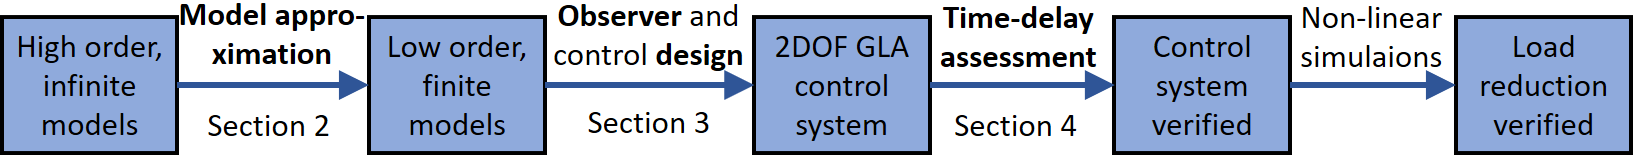
\includegraphics[width=1\textwidth]{strct.png}
	\caption{Proposed tool-chain using advanced mathematical methods for developing a gust load alleviation control system.}
	\label{fig:toolchain}	
\end{figure}






\section{Model approximation}\label{sec:mr}

When dealing with industrial problems such as aircraft systems, associated models usually embed unsteady aerodynamics as well as structural modes and aerodynamical delays. Consequently, the dimension of the  state-space dimensions can be very large, and additionally models can include delays and potentially mixing differential and algebraic equations. Thus, before the methods presented in section \ref{sec:th} can be applied, a pre-processing step, to reduce the state dimension and simplify the complexity should be first applied in order to improve the numerical treatment and accuracy of the results. A short reminder of the methods involved in section \ref{sec:app} are briefly discussed in this section. As these methods are not the main topic of this paper, more details on infinite or data-driven model approximation techniques can be found in \cite{AntoulasSurvey:2016,DalmasECC:2016,Meyer:2016}, and on finite order large-scale model approximation in \cite{AntoulasBook:2005,GugercinSIAM:2008}.  Let us follow these two classes of problems and remind the driving ideas as follows.

\subsection{Infinite  dimensional or data-driven model approximation}\label{sec:app_a}

 
Given an infinite dimensional model $H$, it is possible to obtain the  frequency-domain responses ${\Phi}_i \in \mathds C^{n_y \times n_u}$ for different frequency samples $\omega_i$ ($i = 1, \dots , N$). Then, one can write $H(\imath \omega_i) = {\Phi}_i$. One of the data-driven approach is based on the interpolation framework well defined in \cite{Mayo:2007,AntoulasSurvey:2016}, involving the Loewner matrices. The method consists of an \emph{exact rational model interpolation}, optionally followed by a \emph{reduction procedure}. To this aim, let us first partition the collected data $(\omega_i,{\Phi}_i)_{i=1}^N$ in two disjoint sets as follows ($N=q+k$):
\begin{eq}
	\begin{array}{rcl}
		\imath [\omega_1,\dots , \omega_N] &=& [\mu_1, \dots , \mu_{q}] \cup [\lambda_1, \dots , \lambda_{k}] \vspace{+2mm} \\ ~
		[{\Phi}_1,\dots , {\Phi}_N] &=& [\tilde{v}_1,\dots , \tilde{v}_{q}] \cup [\tilde{w}_1, \dots , \tilde{w}_{k}].
	\end{array}
\end{eq} 
Then, define $l_j \in \mathds C^{n_y\times 1}$ ($j=1,\dots , q$) and $r_i \in \mathds C^{n_u\times 1}$ ($i=1,\dots , k$) the $q$ left and $k$ right tangential directions. Using these tangential directions, let us define $v_j^*=l_j^*\tilde{v}_j \in \mathds C^{1\times n_u}$ and $w_i=\tilde{w}_i r_i \in \mathds C^{n_y\times 1}$ the \emph{left} and \emph{right tangential} data directions, respectively. Based on the left interpolation driving frequencies $\{\mu_i\}_{i=1}^q \in \Cplx$ with left output or tangential directions $\{l_i\}_{i=1}^q \in \Cplx^{n_y}$, producing the left responses $\{v_i\}_{i=1}^q$ and right interpolation driving frequencies $\{\lambda_i\}_{i=1}^k \in \Cplx$ with right input or tangential directions $\{r_i\}_{i=1}^k \in \Cplx^{n_u}$, producing the right responses $\{w_i\}_{i=1}^k$, the objective is to find a model transfer function $\tilde H$ which is a tangential interpolant of the data, \ie, satisfies the following left and right interpolation conditions:
%\begin{eq}
%	\left.
%	\begin{array}{c}
%		\lv_j^*\Htran(\mu_j) = \vv_j^* \\
%		\text{for $j=1,\dots, q$}
%	\end{array}
%	\text{~~and~~}
%	\begin{array}{c}
%		\Htran(\lambda_i)\rv_i = \wv_i \\
%		\text{for $i=1,\dots, k$}
%	\end{array}
%	\right\}.
%	\label{eq:interpContrain}
%\end{eq}
\begin{eq}
	\left.
	\begin{array}{c}
		l_j^*\tilde H(\mu_j) = v_j^* \vspace{+2mm} \\
		\text{for $j=1,\dots, q$}
	\end{array}
	\text{~~~~and~~~~}
	\begin{array}{c}
		\tilde H(\lambda_i)r_i = w_i \vspace{+2mm} \\
		\text{for $i=1,\dots, k$}
	\end{array}
	\right\}.
	\label{eq:interpContrain}
\end{eq}
%
%
The interpolation problem \eqref{eq:interpContrain} can be solved thanks to the Loewner framework (see, \eg, \cite{Mayo:2007}). One of the important property of the Loewner approach is that it encodes the minimal McMillian degree of the interpolation model and its minimal realization order $n$. This then leads to an exact descriptor model interpolating the data, especially useful, when the number of data is very large.

\subsection{Finite dimensional model approximation}\label{sec:app_b}
Once an exact interpolation model $\tilde H$ has been obtained, with potentially large dimension, a second step then consists in approximating this finite order model with a low dimensional one. One common objective in model approximation consists in finding a reduced-order model that well captures the main original input/output dynamical behavior. To address this objective, the (frequency-limited) $\mathcal{H}_2$-norm mismatch error is commonly used, see \eg, \cite{GugercinSIAM:2008,VuilleminPhD:2014}. The resulting approximation problem consists thus in seeking a low order approximation model $\hat H(s)$ of $\tilde H(s)$, such that:
%\begin{eq}
%	\Htranr := \arg \min_{
%		\small
%		%\begin{array}{c}
%		\mathbf G\in\mathcal H_2^{n_y\times n_u} \  \rank(\mathbf G)=r \ll n
%		%\end{array}
%		\normalsize
%	} ||\Htran-\mathbf G||_{\mathcal{H}_{2} \text{ or } \mathcal{H}_{2,\Omega}}.
%	\label{pb:h2}
%\end{eq}
\begin{eq}
	\hat H := \arg \min_{
		\small
		\begin{array}{c}
			G\in\mathcal H_2^{n_y\times n_u} \\  \text{rank}(G)=r \ll n
		\end{array}
		\normalsize
	} ||\tilde H-G||_{\mathcal{H}_{2}}.
	\label{pb:h2}
\end{eq}

Beside the fact that problem \eqref{pb:h2} is non convex and non-linear, some conditions have been proposed to reach the so-called \emph{first order optimality conditions} and procedures to ensure that a local (hopefully global) optimum is reached. Moreover, the proposed IRKA and FL-ISTIA algorithms are appropriate to practically tackle these problems (see \eg, \cite{GugercinSIAM:2008,VuilleminPhD:2014} for details). %As  emphasized by the following theorem and corollary, this optimum can be reached thanks to interpolatory methods \cite{GugercinSIAM:2008}. %Let briefly recall and discuss the main results, stated for MIMO LTI DAE models, as follows.
Finally, the derived  model $\hat H$ can be easily brought into the form (\ref{eq:sys}) by separating the inputs accordingly.









\section{Disturbance estimator design}\label{sec:th}
In this section a robust disturbance estimator design problem is derived. The proposed approach is a combination of the proposed nullspace based method for disturbance estimation in \cite{Ossmann18ccta} and the idea of deriving robust filters via optimization \cite{Varga_11, OssVar_13_eucass}.
Thus, in a preliminary step the structure of the disturbance estimator is determined using nullspace based techniques proposed for the disturbance estimator design in \cite{Ossmann18ccta} applied on a set of linear design models. The extracted  structure from this linear design is then optimized to solve the multi model design problem applying a non-linear optimization techniques similar to the approaches described in \cite{Varga_11, OssVar_13_eucass}.

\subsection{Problem formulation}
Consider the set of linear models described by the input-output form
\begin{equation}\label{eq:sys}
	y^{(i)}(s) = G_u^{(i)}(s) u(s) + G_{n}^{(i)}(s) n(s)  + G_d^{(i)}(s) d(s),
\end{equation}
where $y^{(i)}(s)$, $u(s)$, and $n(s)$  are the Laplace-transformed
vectors of the $p$-dimensional system output vector $y^{(i)}(t)$, the $m_u$-dimensional control input vector $u(t)$, and the $m_{n}$-dimensional noise vector $n(t)$, respectively. The noise vector includes any non-measurable disturbances which are need to be decoupled from the estimate. $d(s)$ is the Laplace-transformed of the scalar  disturbance input $d(t)$ to be estimated.
$G_u^{(i)}(s)$, $G_{n}^{(i)}(s)$, and $G_d^{(i)}(s)$ are the transfer-function matrices (TFMs) from control inputs to  outputs, noise inputs to outputs, and disturbance  to outputs, respectively.  The index ${(i)}$ is used to describe the set of $i=1,\dots, N$ linear models which are linearized on different trim points.

The design goal is to derive a single linear disturbance estimator $O(s)$ which processes the measurable system outputs $y^{(i)}(t)$ and control inputs $u(t)$ and generates the disturbance estimate $\tilde d(t)$. In the input-output form this can be described by
\begin{equation}\label{eq:est}
	\tilde d^{(i)}(s) = O(s)
	\begin{bmatrix}
		y^{(i)}(s) \\ u(s)
	\end{bmatrix},
\end{equation}
where $O(s)$ is the disturbance estimator TFM. Note that the robustness aspects come into play as we search for a single filter $O(s)$ valid for all the $N$ available design models.
The order of $O(s)$ is the dimension of the state vector of a minimal state-space realization of $O(s)$.
From the general description in (\ref{eq:est}) follows the definition of the robust disturbance estimation problem (RDEP): Design a physically realizable, stable, and linear disturbance estimator of the form (\ref{eq:est}) such that 
\begin{equation}\label{eq:rdep}
	\begin{array}{lll}
		(a) & \tilde d^{(i)}  \approx 0 &\text{when } d = 0  \,\, \forall  \,\, \{u, n \} \text{  for  } i=1,\dots,N\\ 
		(b) &\tilde d^{(i)} \approx d &\text{when } d \neq 0 \,\, \text{  for  } \,\, i=1,\dots,N 
	\end{array}
\end{equation}
Note that in (\ref{eq:rdep}) an approximated form is used, i.e. the estimate shall be approximately zero when for any control and noise input. In case of such a multi-model formulation an exact decoupling over all models generally cannot be achieved. The remainder of this section focuses on a strategy how the RDEP can be numerically solved.



\subsection{Solving the robust disturbance estimation problem}\label{sec:rdep}
The design of the robust disturbance estimator $O(s)$ which allows the estimation of the gust for all $N$ models is done in two steps. In the first step the structure of the disturbance estimator is determined, solving a dedicated disturbance estimation problem (DEP) for each model independently. In the second step this structure is extracted and used within an optimization algorithm to determine the optimal parameter ensuring the required conditions $(a)$ and $(b)$.

\subsubsection{Estimator Structure}\label{sec:strc}
The structure of the disturbance estimator is determined by solving the DEP \cite{Ossmann18ccta} for each model individually. In this case the computation relies on advanced nullspace techniques \cite{}. Let us first consider the $i^{\text{th}}$-model  for which the  $i^{\text{th}}$- disturbance  estimator 
\begin{equation}\label{eq:estr}
\tilde d^{(i)}(s) =  O^{(i)}
\begin{bmatrix}
y^{(i)}(s) \\ u(s)
\end{bmatrix}
\end{equation}
can be designed.
Inserting the  model equation (\ref{eq:sys})  into (\ref{eq:estr}) leads to
\begin{equation}\label{eq:full}
\tilde d^{(i)}(s) = O^{(i)}(s) 
\begin{bmatrix}
G_u^{(i)}(s) & G_{n}^{(i)}(s) & G_d^{(i)}d(s) \\ I_{m_u}& 0 & 0
\end{bmatrix}
\begin{bmatrix}
u(s) \\ n(s) \\ d(s)
\end{bmatrix},
\end{equation}
describing the  $i^{\text{th}}$ disturbance estimate $\tilde d^{(i)}(s)$ in dependence of the control, noise and disturbance inputs.  If the DEP can be solved exactly, we adapt the requirements $(a)$ and $(b)$ of the RDEP to the DEP following \cite{Ossmann18ccta} to
\begin{equation}
\begin{array}{lll}
(\tilde a) & \tilde d = 0 & \text{when } d = 0  \,\, \forall  \,\, \{\, u, n \}\\ 
(\tilde b) &\tilde d \approx d & \text{when } d \neq 0, 
\end{array}
\end{equation}
demanding an exact decoupling of the control inputs $u$ and the noise $n$ from the disturbance estimate in $(\tilde a)$ and an approximative estimation of the disturbance $d$ in $(b)$ 

Next, the formulated requirements in $(\tilde a)$ and $(\tilde b)$ can be transformed into  algebraic conditions. 
The decoupling condition $(a)$ requires that the disturbance estimate $\tilde d(s)$ is decoupled from all inputs $u(s)$ and noise $n(s)$. This is equivalent of demanding 
\begin{equation}\label{eq:ns}
O^{(i)}(s) 
\begin{bmatrix}
G_u^{(i)}(s) & G^{(i)}_{n}(s)  \\ I_{m_u}& 0
\end{bmatrix}
:= O^{(i)}(s) G_e^{(i)}(s) =  0.
\end{equation}
It follows that $O^{(i)}(s)$ needs to be a left annihilator of $G_e^{(i)}(s)$. 
By deriving a minimal basis $N_l^{(i)}(s)$ for the left nullspace of $G_e^{(i)}(s)$,  the design conditions $(\tilde a)$ can be tackled. For design condition $(\tilde b)$, the basic constraint
\begin{equation}\label{eq:c2}
O^{(i)}(s) 
\begin{bmatrix}
G_{d}^{(i)}(s)  \\  0
\end{bmatrix}
\neq  0
\end{equation}
must be fulfilled to ensure the estimate-ability of the disturbance. If or not the DEP in (\ref{eq:ns}) and (\ref{eq:c2}) can be solved exactly is based on  necessary and sufficient rank criteria. As for realistic design problems this condition is often fulfilled, it is nor further discussed herein. Interested readers are referred to \cite{Var09, Ossmann18ccta, Varga17}.

The required nullspace computation in (\ref{eq:ns})  can  be solved readily available using numerical tools \cite{Varga17}. If the DEP is solvable, a disturbance estimator can be constructed from the nullspace basis ensuring (\ref{eq:c2}) as well as the minimal order of the resulting estimator. In this design procedure, the actual dynamics of the estimator are a design freedom, i.e. the poles of the filter can be freely chosen.

At this point of the design approach, the DEP has been solved for each of the $N$ models individually. As the underlying models often exhibit the same model structure, a common filter structure can be extracted. In words, if a specify entry
of the $N$ state space matrices features the same value over all $N$ models (e.g. 0), this value is kept constant during the optimization process of the robust estimator, reducing the complexity of the proposed optimization.

\subsubsection{Parameter Tuning}\label{sec:tuning}
Having defined the structure and the free parameters $K$ of the estimator $O(s)$ in (\ref{eq:est}), the net task is to optimally tune these free parameters $K$ of the estimator. As criteria a $H_\infty$ norm optimization is selected for which numerical tools in \matlab are available. The disturbance estimator shall ensure the conditions defined in (\ref{eq:rdep}). The goal is to design a single estimator which decouples the control inputs and the noise for all $N$ models. As this can seldom be solved exactly, i.e. the decoupling condition (\ref{eq:ns}) cannot be fulfilled for all N models with a single estimator, we use the reformulation of the problem based on the $H_\infty$ norm. Thus, the decoupling requirement $(a)$ is expressed as  multi-model norm condition for  $i=1,\dots,N$ by
\begin{equation}\label{eq:rc1}
||O(s) \, G_e^{(i)}(s) ||_\infty  \,\approx 0.
\end{equation}
Similar, the disturbance coupling requirement $(b)$ is reformulated as multi-model model matching problem  $i=1,\dots,N$ as
\begin{equation}\label{eq:rc2}
|| O(s) \, [ G_d^{(i)}(s) \,\, 0 ]^T - M(s) ||_\infty \,\approx 0,
\end{equation}
where $M(s)$ defines the desired estimation dynamics. Finally, to determine the free parameters $P$ of the disturbance estimator $O(s)$ the conditions (\ref{eq:rc1}) and (\ref{eq:rc2}) are turned into the non-convex, non-smooth optimization problem
\begin{equation} \label{eq:opt}
\begin{array}{l}
\min_{P} \, \max_{i} \, || \, O(s,P) \, G_e^{(i)}(s) \, ||_\infty \vspace{+2mm} \\
\textnormal{s.t. } ||\, O(s,P) \,\, [ G_d^{(i)}(s) \,\, 0 ]^T - M(s) \, ||_\infty < \gamma \vspace{+2mm} \\
P_{\min} < P < P_{\max},
\end{array}
\end{equation}
for $i=1,\dots,N$, where $P_{\min}$ and $P_{\max}$ are the minimum and maximum values of the tuning parameters and $\gamma$ is a parameter to define the accuracy of the disturbance estimate. The optimization problem in (\ref{eq:opt}) can be  solved numerically using standard Matlab tools as for example the \texttt{systune} command.


\textcolor{red}{
\section{Stability assessment}\label{sec:st}
Charles with some theory about the assessment
}

\section{Application}\label{sec:app}
The proposed methods in the the last sections are applied to a a generic example of a medium size business jet 
for which a detailed model of the rigid body dynamics, aerodynamics as well as structural dynamics is available.
The model of the aircraft is divided into subsections, i.e. the front section, a middle section including the wings, and a rear section with the elevators and the aircraft's tail, so that the effect of an incoming gust can be realistically modeled. Each section features three gusts inputs, one for the actual gust and its two derivatives in time which are required to realistically model the unsteady aerodynamics. Having  gust inputs for each aircraft sections enables, for example, a delayed injection of a gust for each part  so that the gust can hit the different sections of the aircraft one after the other and mimic a realistic behavior.
 
To  compute and compare loads with  and without load alleviation controller an aircraft model with about 300 states  is available. Besides the basic aircraft dynamics, the model also includes realistic actuator and sensor models as well as a baseline control law, providing adequate handling qualities to the pilot.
The control inputs to the open loop aircraft model are the  commands of the elevator, the inner ailerons and the outer ailerons. 
The gust impact on the model is characterized by  nine inputs describing the position, velocity and acceleration impact at three different locations along the fuselage.
As measured signals for feedback control, the pitch rate, the load factor,  and the angle of attack are provided.
The provided baseline controller only commands the elevator, while  the load alleviation controller shall use the ailerons symmetrically to alleviate the bending moments due to gusts.

In the following subsections a low order model for the estimator design is derived first in section \ref{APPsubsec:model}  applying the techniques presented in section
\ref{sec:mr}. Then, a disturbance estimator is derived following the approach in section \ref{sec:th}, including the point wise estimator design from subsection \ref{sec:strc} to derive the filter structure followed bz solving the RDEP by the optimization presented in subsection \ref{sec:tuning}. In the same section a simple proportional feedback law from the disturbance estimate to the ailerons is presented to close the loop.
The stability of the closed loop is assessed in section \ref{APPsubsec:stab} and simulations results using the high fidelity benchmark model are reported in \ref{APPsubsec:sim}.

\subsection{Model approximation}\label{APPsubsec:model}
Ten LTI aircraft models, each of about 300 states, linearized on 10 different trim points in the flight envelope, i.e. different speeds and altitudes, and weight and balance domain, i.e., different masses and center of gravity positions, are available.
The high number of states as well as nine gust inputs of the models makes the 
estimator and control design challenging. Thus the idea is to reduce the state dimension and the number  of disturbance inputs. In view of disturbance estimator and control design, it is preferable to use a single disturbance single input.
The nine disturbance inputs are used in the available simulation to model a \textit{single} gust hitting  three different sections  (front, middle, rear) of the aircraft one after another. The derivatives of the three gust input positions are required to consider the unsteady aerodynamics. 
Consequently, the second and third set of gust inputs are equal to the first one but delayed by a fixed time delay. Thus, mathematically the second and third set of inputs can be derived by simply delaying the first on. Additionally, the velocity and acceleration of the first gust input can be derived by derivative action on the first gust input position, finally reducing the gust inputs to a single one.
%After these modifications, the resulting model now embeds two internal delays (denoted $\tau_1$ and $\tau_2$, related to the velocity of the aircraft and patch where the gust is impacting the fuselage) and have a rank deflective descriptor form. These internal delays are explained by the use of exact delay actions applied on the exact derivative terms. As a consequence, at this stage, the linear time-invariant dynamical system can be represented by  first order descriptor realization with $n_u$ inputs (one signle gust niput), $n_y$ outputs, $n$ internal variables and two internal delays. The model is given by a set of differential and algebraic equations (\textbf{DAE}) where states are described by $\E\dx(t) =\A_0 \x(t) + \A_1 \x(t-\tau_1)+ \A_2 \x(t-\tau_2) +\B \u(t)$ (with $\E$ rank deflective) and outputs $\y(t) = \C \x(t)$, where, $\x(t) \in \Real^{n} := \mathcal X$ is the internal variables, and $\u(t) \in \Real^{n_u} := \mathcal U$ and $\y(t) \in \Real^{n_y} := \mathcal Y$ are the input, output functions, respectively, while $\E,\A_0,\A_1,\A_2 \in \mathds{R}^{n \times n}$, $\B \in \mathds{R}^{n\times n_u}$ and $\C \in \mathds{R}^{n_y \times n}$ are constant matrices. The matrix pencil is regular if the matrix $(\A_0 +\A_1e^{-\tau_1\lambda}+\A_2e^{-\tau_1\lambda}) - \lambda\E$ is non-singular for some finite $\lambda \in \Cplx$ and a $\{\tau_1,\tau_2\}$ couple. In this case, the associated transfer function is
After these modifications, the resulting models now embed two internal delays (denoted $\tau_1$ and $\tau_2$, related to the velocity of the aircraft) and have a rank deflective descriptor form. These internal delays are explained by the use of exact delay actions applied on the exact derivative terms. Thus, the linear time-invariant dynamical systems can be represented by a first order descriptor realizations with $n_u$ inputs (including one single gust input), $n_y$ outputs, $n_x$ internal variables, and the two internal delays. The $N=10$ models are given by sets of differential and algebraic equations for $i=1,\dots,N$  by
\begin{eq}
	\begin{array}{rcl}
		E^{(i)} \dot x^{(i)}(t) &=&\A^{(i)}_0 x(t) + \A^{(i)}_1 x(t-\tau_1)+ \A^{(i)}_2 x^{(i)}(t-\tau_2) +\B^{(i)} u(t) \vspace{+2mm} \\
		y^{(i)}(t) &=& \C^{(i)} x^{(i)}(t),
	\end{array}
\end{eq}
with the  rank defective matrix $E^{(i)}$,  the internal variables
$x^{(i)}(t) \in \Real^{n_x} := \mathcal X$, and  the input and output functions $u(t) \in \Real^{n_u} := \mathcal U$ and $y^{(i)}(t) \in \Real^{n_y} := \mathcal Y$, respectively.  $E^{(i)},\A^{(i)}_0,\A^{(i)}_1,\A^{(i)}_2 \in \mathds{R}^{n_x \times n_x}$, $\B^{(i)} \in \mathds{R}^{n_x \times n_u}$ and $\C^{(i)} \in \mathds{R}^{n_y \times n_x}$ are constant matrices. 
Note, we assume equivalent time delays $\tau_1$ and $\tau_2$ for all 10 models.

The matrix pencil is regular if the matrix $(\A_0^{(i)} +\A_1^{(i)}e^{-\tau_1\lambda}+\A_2^{(i)}e^{-\tau_1\lambda}) - \lambda E^{(i)}$ is non-singular for some finite $\lambda \in \Cplx$ and a $\{\tau_1,\tau_2\}$ couple. In this case, the associated transfer functions are
\begin{eq}
	H^{(i)}(s) = \C^{(i)}\big(s E^{(i)}-\A^{(i)}_0-\A^{(i)}_1e^{-\tau_1s}-\A^{(i)}_2e^{-\tau_2s}\big)^{-1}\B^{(i)} + D^{(i)}.
\end{eq}
Obviously, due to the presence of delays in the dynamical part of the equations, the resulting model is now of infinite dimension. To cope with this,  first  an exact stable Loewner interpolation of this infinite model by a finite order one is performed as discussed in section \ref{sec:app_a}. This leads to a large scale descriptor model of dimension $n$, which exactly interpolates the infinite dimensional models $H$, with $\tilde{H}(s)$, of the form
\begin{eq}
	\tilde{H}^{(i)}(s) = \tilde{\C}^{(i)}\big(s\tilde{E}^{(i)}-\tilde{\A}^{(i)}\big)^{-1}\tilde{\B}^{(i)}.
\end{eq}
Now, this finite order models (\eg with a finite number of eigenvalues) can be readily approximated using any (frequency-limited) $\mathcal H_2$ oriented model approximation techniques as discussed in section \ref{sec:app_b} and further presented in \eg, \cite{GugercinSIAM:2008,VuilleminSSSC:2013,PoussotMORE:2012}. This leads to  reduced order models with dimension $r\ll n$, as, 
\begin{eq}
	\hat H^{(i)}(s) = \Cr^{(i)}\big(s\Er^{(i)}-\Ar^{(i)}\big)^{-1}\Br^{(i)}
\end{eq}
which minimize the (frequency-limited)  mismatch error. 
Finally, the 10 aircraft models each of about 300 states with nine disturbance inputs have been approximated with 10 models each of order $r=25$ with a single disturbance input. These reduced models can now be used to design the disturbance estimator. 


\subsection{Gust load alleviation system}\label{APPsubsec:sys}
The two degree of freedom gust load alleviation system consists of the disturbance estimator designed with the approaches in section \ref{sec:th} and a simple control law. In the following the disturbance estimator as well as the controller is designed for the business jet aircraft. For the estimator design the reduced order models derived in section \ref{APPsubsec:model} are used. The control law is a simple feedback of the estimated gust to the symmetric aileron deflection. Note that only the ailerons are used to mitigate the gust loads. The ailerons only induce, due to their proximity to the center of gravity in the longitudinal direction, a neglectable pitching  moment. This minimizes the influence of the additional control law on the handling qualities provided to the pilot.

\begin{figure}[h]
	%\centering
	\sidecaption[]
	%\usetikzlibrary{positioning,plotmarks, matrix, arrows, calc, shapes}
\tikzstyle{blockdiag}	= [node distance=5mm, >=stealth', semithick]
\tikzstyle{block}			= [draw, rectangle, minimum width=1.05cm, minimum
height=.8cm]


\tikzstyle{block2}			= [draw, rectangle, minimum width=1.05cm, minimum
height=.8cm, fill=white]

\tikzstyle{sum} = [draw,circle,inner sep=0pt, minimum size=6pt]
\tikzstyle{connector} = [draw,circle,inner sep=0pt, minimum size=0.001pt, 
fill=black]
\tikzstyle{connector2} = [draw,circle,inner sep=0pt, minimum size=2pt, 
fill=black]
\tikzstyle{gain} = [draw,regular polygon, regular polygon 	sides=3,thick,minimum height=3em,minimum width=4em, rotate=30]
\tikzstyle{bguide} = [rectangle,minimum height=3em,minimum	width=4em]
\tikzstyle{line} = [thick]
\tikzstyle{branch} = [circle,inner sep=0pt,minimum size=1mm,fill=black,draw=black]
\tikzstyle{guide} = [anchor=center]

\pgfdeclarelayer{bg}    % declare background layer
\pgfsetlayers{bg,main}

\begin{tikzpicture}[blockdiag, auto, scale=0.8]

% Blocks
\node[block,minimum width=1.25cm, minimum height=1.5cm](Plant) {$G$};
\node[block, minimum width=1.25cm, minimum height=1cm,left=of Plant, xshift=-1.5cm, yshift=0.47cm] (C) {$C_\eta$};
\node[block, minimum width=1.25cm, minimum height=1cm,below=of Plant,  yshift=0cm] (Obsv) {\textcolor{blue}{$O_e$}};
%\node[block, minimum width=1cm, minimum height=.8cm,below=of Obsv,  yshift=-0.2cm] (logic) {$> \tau_{th}$};
\node[block2, minimum width=1.25cm, minimum height=1cm,left=of Obsv, xshift=-1.5cm, yshift=0.5cm] (Cload) {\textcolor{blue}{$C_{\Delta \xi}$}};


\node[connector2, right=of Plant, xshift = 0.65cm] (con1) {}; 
\node[connector2, right=of Plant, xshift = 0.25cm, yshift = 0.5cm] (con2) {}; 
\node[connector2, right=of Cload, xshift = 0.65cm, yshift = -0.23cm] (con3) {}; 
\node[connector2, right=of Cload, xshift = 0.25cm, yshift = 0.25cm] (con4) {}; 
\node[connector2, right=of C, xshift = 1cm] (con5) {}; 
\node[connector, below=of Cload, xshift = -0.5cm, yshift = 0.2cm] (con6) {}; 
\node[connector, above=of Cload, xshift = 0.5cm, yshift = -0.2cm] (con7) {}; 
\node[connector, right=of Plant, xshift = 0.1cm, yshift = -0.5cm] (con8) {}; 
\node[connector, below=of Obsv, xshift = 0cm, yshift = -0.0cm] (con9) {}; 

\draw[->]  (Plant.east) ++(0cm,0.6cm)  --  ++(1cm,0cm) node[pos=0.27,yshift=-1mm] {$q$} --  ++(0cm,1.60cm)  -| ($(C.north)+(0.4cm,0cm)$);
\draw[->]  (Plant.east) ++(0cm,0cm)  --  ++(1.5cm,0cm) node[pos=0.27,yshift=-1mm] {$n_z$}  --  ++(0cm,2.60cm)   -|  ($(C.north)-(0.4cm,0cm)$);

\draw[->]  (Cload.east) ++(0cm,0.3cm)  --  ++(1.0cm,0cm) node[pos=0.39,yshift=-.5mm] {\textcolor{blue}{$\Delta \xi_i$}}    |- ($(Plant.west)+(0cm,0cm)$);
\draw[->]  (Cload.east) ++(0cm,-0.3cm)  --  ++(1.5cm,0cm) node[pos=0.29,yshift=-.5mm] {\textcolor{blue}{$\Delta  \xi_o$}}    |- ($(Plant.west)+(0cm,-0.6cm)$);

\draw[->]  (C)  --  ($(Plant.west)+(0cm,0.59cm)$)node[pos=0.13]{$\eta$};
\draw[->]   (con9) -| (Cload.south);
\draw[<-, color=red] (Plant.north) -- +(0cm, +1cm)node[left, pos=.7]{\textcolor{red}{$d$}};

\draw[->]  (con1)  |-  ($(Obsv.east)+(0cm,-0.5cm)$);
\draw[->]  (con2)  |-  ($(Obsv.east)+(0cm,0cm)$);
\draw[->]  (con8)  |-  ($(Obsv.east)+(0cm,+0.5cm)$);


\draw[->]  (con5)  |-  ($(Obsv.west)+(0cm,0.5cm)$);
\draw[->]  (con4)  |-  ($(Obsv.west)+(0cm,0cm)$);
\draw[->]  (con3)  |-  ($(Obsv.west)+(0cm,-0.5cm)$);


\draw[-]  (con9)  --  (Obsv)node[pos=0.75,yshift=-1mm] {\textcolor{blue}{$\tilde d$}};
\draw[-]  (Plant.east)++(0cm,-0.625cm)   --  (con8)node[pos=0.4,yshift=-.5mm] {$\alpha$};
%\draw[->]  (con8)  -- ++(0.0cm,-4.5cm)  -- ++(-8.5cm,0cm)  |-  (Cload.west);

;\end{tikzpicture} 
	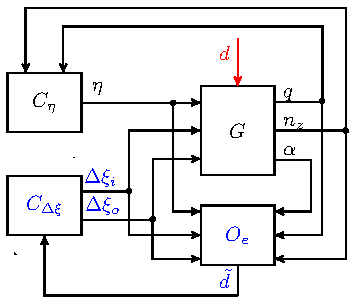
\includegraphics{closedloop.pdf}
	\caption{Closed loop structure including aircraft dynamics $G$, baseline controller $C_\eta$, disturbance estimator $O$, and  load alleviation controller $C_{\Delta \xi}$. }
	\label{fig:cl}	
\end{figure}

A disturbance estimator with the presented methods in section \ref{sec:th} is designed for the aircraft. The  $N=10$ design models after the model approximation features 25 states, three control inputs, namely elevator, symmetric inner aileron and symmetric outer aileron position, one gust input and the two measurable outputs, \ie,  pitch rate and the load factor. For the  10 available aircraft models, 10 disturbance estimators are derived and the common structure is extracted.
A common dynamic for the 10 resulting first order disturbance estimators is chosen at 0.1\,s, i.e. a pole at -10. This value allows a fast estimation of the incoming disturbance.
Finally, applying the optimization step presented in section \ref{sec:tuning}  results in the disturbance estimator $O$ with the state space realization
\begin{equation}\label{eq:obs}
	\begin{array}{rcr}
		\dot  x_e  &=& -10 x_e + B_e
		\begin{bmatrix}
			q & n_z & \alpha & \eta & \xi_i & \xi _o 
		\end{bmatrix}^T \,\,\, \vspace{+1mm} \\ 
		\tilde d &=&  x_e + 
		D_e
		\begin{bmatrix}
			q & n_z & \alpha & \eta & \xi_i & \xi _o 
		\end{bmatrix}^T,
	\end{array}
\end{equation}
with  
\begin{equation*}
\begin{array}{rcl}
B_e &=&
\begin{bmatrix}
  \, -2 &   0.32 &   -14.85 &   0.05 &   0.07 &  0.023 \,
\end{bmatrix}  \,\,\, \vspace{+2mm} \\
 D_e &=&
\begin{bmatrix}
  \, 0.05  &  0   &1.5 &0 &  0 &  0 \,
\end{bmatrix}. 
\end{array}
\end{equation*}
Note that the zero elements in $D_e$ are kept 0 during the  optimization step. The zeros are common in all 10 disturbance estimators determined in the preliminary design step to extract the estimator structure.
The disturbance estimator is discretized for the implementation in the high-fidelity simulation model with 80\,Hz using a standard Tustin approximation.
The sampling rate of 80\,Hz correspond to the sampling rate available in the flight control computer on the actual aircraft.


Having an estimate of the gust available, the estimate is feed back to symmetric aileron deflections to counteract the gust, i.e., 
\begin{equation}	
	\begin{bmatrix}
		\Delta \xi_i \\ \Delta \xi_o 
	\end{bmatrix} = 
 	C_{\Delta\xi}
	\tilde d 
	=
	\begin{bmatrix}
		k_{\xi_i}(s) \\ k_{\xi_o}(s) 
	\end{bmatrix}
	\tilde d.
\end{equation}
For this paper, constant gains between 0.75 and 1.5 have been selected for $k_{\xi_i}$ and $k_{\xi_o}$ for which the stability assessment is performed in the next section.

%The overall structure of the closed loop system is depicted in Fig. \ref{fig:cl}. The baseline controller $C_\eta$ uses the measurements load factor $n_z$ and the pitch rate $q$ from the aircraft $AC$ as inputs to generate the elevator deflection $\eta$. It ensures adequate handling and disturbance rejection in the longitudinal, rigid body motion of the aircraft. The disturbances $d$ are acting on the aircraft as unknown inputs. The aircraft in this illustration also includes the sensor and actuator dynamics.



\textcolor{red}{
\subsection{Stability Assessment}\label{APPsubsec:stab}
Charles with results from the benchmark
}

\subsection{Simulation based load verification}\label{APPsubsec:sim}
The developed gust load alleviation system is verified in a high-fidelity non-linear simulation model of the medium sized business jet. It features the full order dynamics of the aircraft, as well as detailed sensor model with anti-aliasing filter, non-linear actuator models, the baseline control law for the longitudinal axis. The whole flight control system is simulated in discrete from with a sample rate of 80\,Hz.

Due to the detailed structural model, the loads on six dedicated position on each wing can be determined. For the work herein, the wind bending moments will be computed as these are the predominant loads for sizing the structure of the aircraft.
The gust scenario is an 1-cosine gust \cite{Flomenhoft94,Fuller95}, hitting the aircraft first at the front from either with an upward or downward wind velocity and making its way over the three sections of the aircraft.
The required gust inputs are computed within the simulation internally for the three sections of the aircraft. The user needs to only define the  wavelength of the 1-cosine gust to be simulated.  Different gust wavelength between approximately 27.5\,m and 46\,m are considered. The vertical wind speed of each gust is a function of altitude and aircraft speed and is also computed internally, lying between about 10\,m/s and 16.5\,m/s.

First, to verify the disturbance estimator, the capability of estimating the gusts, the model is simulated with an open gust alleviation loop. Figure \ref{fig:est} shows the estimated gust in comparison to the actual gusts for all 10 available trim points. The first diagram shows the results for a selected wavelength of  27.5\,m, the second diagram for 34.7\,m, and the third on for 46\,m. The selected wavelength of 34.7\,m is chosen as it is defined to be the sizing wavelength for this aircraft. Note the changing gust amplitudes for a constant wavelength setting in the diagrams of figure \ref{fig:est}.

\begin{figure}[hbt]
	%\centering
	\sidecaption[]
	% This file was created by matlab2tikz.
%
%The latest updates can be retrieved from
%  http://www.mathworks.com/matlabcentral/fileexchange/22022-matlab2tikz-matlab2tikz
%where you can also make suggestions and rate matlab2tikz.
%
\definecolor{mycolor1}{rgb}{0.97650,0.58870,0.35690}%
\definecolor{mycolor2}{rgb}{0.91563,0.80613,0.36568}%
\definecolor{mycolor3}{rgb}{0.80000,0.92550,0.35290}%
\definecolor{mycolor4}{rgb}{0.60271,0.92423,0.32717}%
\definecolor{mycolor5}{rgb}{0.36230,0.89170,0.28580}%
\definecolor{mycolor6}{rgb}{0.28636,0.81217,0.49968}%
\definecolor{mycolor7}{rgb}{0.21990,0.71340,0.72250}%
\definecolor{mycolor8}{rgb}{0.33376,0.57025,0.90699}%
\definecolor{mycolor9}{rgb}{0.42960,0.38580,0.99220}%
\definecolor{mycolor10}{rgb}{0.50769,0.14203,0.79906}%
%
\begin{tikzpicture}
\begin{axis}[%
width=2in,
height=0.80in,
at={(0in,0in)},
scale only axis,
xmin=0.75,
xmax=2,
ymin=-4,
xtick = {\empty},
ymax=4,
ylabel={$d$, $\tilde d$ (deg)},
ylabel style={yshift=-2mm},
axis background/.style={fill=white}
]
\addplot [color=mycolor1,solid,line width=2.0pt,forget plot]
  table[row sep=crcr]{%
0	0\\
0.991666666666667	0\\
1	0.000188757916213942\\
1.00833333333333	0.000188757916213942\\
1.01666666666667	0.0130712610274747\\
1.025	0.097792806989399\\
1.03333333333333	0.097792806989399\\
1.04166666666667	0.324707514686646\\
1.05	0.713650443402219\\
1.05833333333333	0.713650443402219\\
1.06666666666667	1.21557524568106\\
1.075	1.75365779743446\\
1.08333333333333	1.75365779743446\\
1.09166666666667	2.24890856173775\\
1.1	2.63103873743934\\
1.10833333333333	2.63103873743934\\
1.11666666666667	2.85501734344068\\
1.125	2.8862257774489\\
1.13333333333333	2.8862257774489\\
1.14166666666667	2.71083977616121\\
1.15	2.33620135898828\\
1.15833333333333	2.33620135898828\\
1.16666666666667	1.77350645382994\\
1.175	1.05857169716816\\
1.18333333333333	1.05857169716816\\
1.19166666666667	0.251946021952037\\
1.2	-0.573830180835068\\
1.20833333333333	-0.573830180835068\\
1.21666666666667	-1.34771530755664\\
1.225	-2.01925615298324\\
1.23333333333333	-2.01925615298324\\
1.24166666666667	-2.55063800949914\\
1.25	-2.90746248992307\\
1.25833333333333	-2.90746248992307\\
1.26666666666667	-3.06153216370768\\
1.275	-2.99753808969362\\
1.28333333333333	-2.99753808969362\\
1.29166666666667	-2.7333191376626\\
1.3	-2.35207549753526\\
1.30833333333333	-2.35207549753526\\
1.31666666666667	-1.9620144937005\\
1.325	-1.63417117379391\\
1.33333333333333	-1.63417117379391\\
1.34166666666667	-1.38180870446494\\
1.35	-1.18937070494871\\
1.35833333333333	-1.18937070494871\\
1.36666666666667	-1.02779890665553\\
1.375	-0.869666801409095\\
1.38333333333333	-0.869666801409095\\
1.39166666666667	-0.71192939385732\\
1.4	-0.560710644657563\\
1.40833333333333	-0.560710644657563\\
1.41666666666667	-0.428179861188562\\
1.425	-0.318709494886045\\
1.43333333333333	-0.318709494886045\\
1.44166666666667	-0.214420669600296\\
1.45	-0.108156831590921\\
1.45833333333333	-0.108156831590921\\
1.46666666666667	-0.0114647368980467\\
1.475	0.0586973589931954\\
1.48333333333333	0.0586973589931954\\
1.49166666666667	0.0938370375408674\\
1.5	0.107359440410918\\
1.50833333333333	0.107359440410918\\
1.51666666666667	0.118300848788176\\
1.525	0.13664500490694\\
1.53333333333333	0.13664500490694\\
1.54166666666667	0.165278183374462\\
1.55	0.20349205587767\\
1.55833333333333	0.20349205587767\\
1.56666666666667	0.246669421626506\\
1.575	0.282016056070105\\
1.58333333333333	0.282016056070105\\
1.59166666666667	0.296972169990529\\
1.6	0.29405697813143\\
1.60833333333333	0.29405697813143\\
1.61666666666667	0.289087292039654\\
1.625	0.28981386109089\\
1.63333333333333	0.28981386109089\\
1.64166666666667	0.283951723226308\\
1.65	0.255409932244534\\
1.65833333333333	0.255409932244534\\
1.66666666666667	0.206972871840712\\
1.675	0.16128722022707\\
1.68333333333333	0.16128722022707\\
1.69166666666667	0.137765150472063\\
1.7	0.135705779704713\\
1.70833333333333	0.135705779704713\\
1.71666666666667	0.143418665121777\\
1.725	0.154945041325129\\
1.73333333333333	0.154945041325129\\
1.74166666666667	0.170686180919815\\
1.75	0.187768031934511\\
1.75833333333333	0.187768031934511\\
1.76666666666667	0.200536515688792\\
1.775	0.208404514736446\\
1.78333333333333	0.208404514736446\\
1.79166666666667	0.216526499397438\\
1.8	0.226191164377102\\
1.80833333333333	0.226191164377102\\
1.81666666666667	0.227657710926491\\
1.825	0.209391568106758\\
1.83333333333333	0.209391568106758\\
1.84166666666667	0.173744996765039\\
1.85	0.137613765304049\\
1.85833333333333	0.137613765304049\\
1.86666666666667	0.11519221046388\\
1.875	0.104272855056926\\
1.88333333333333	0.104272855056926\\
1.89166666666667	0.0930469183859542\\
1.9	0.0759428990162907\\
1.90833333333333	0.0759428990162907\\
1.91666666666667	0.0587813748861445\\
1.925	0.0497107035603942\\
1.93333333333333	0.0497107035603942\\
1.94166666666667	0.0491935454691822\\
1.95	0.0520204876389087\\
1.95833333333333	0.0520204876389087\\
1.96666666666667	0.0557858801985472\\
1.975	0.0618037220165355\\
1.98333333333333	0.0618037220165355\\
1.99166666666667	0.0690809718551232\\
2	0.073638022432026\\
2.00833333333333	0.073638022432026\\
2.01666666666667	0.0751378283511413\\
};
\addplot [color=mycolor2,solid,line width=2.0pt,forget plot]
  table[row sep=crcr]{%
0	0\\
0.00833333333333333	0\\
0.991666666666667	0\\
1	0.000205090319999076\\
1.00833333333333	0.000205090319999076\\
1.01666666666667	0.0141292511979444\\
1.025	0.105561049204391\\
1.03333333333333	0.105561049204391\\
1.04166666666667	0.349917800475761\\
1.05	0.766976222293618\\
1.05833333333333	0.766976222293618\\
1.06666666666667	1.30039336717826\\
1.075	1.86233364086984\\
1.08333333333333	1.86233364086984\\
1.09166666666667	2.36559985184088\\
1.1	2.73475090003904\\
1.10833333333333	2.73475090003904\\
1.11666666666667	2.92225653957986\\
1.125	2.89247458368139\\
1.13333333333333	2.89247458368139\\
1.14166666666667	2.63443053606789\\
1.15	2.16264681502936\\
1.15833333333333	2.16264681502936\\
1.16666666666667	1.49963765867031\\
1.175	0.695621345110457\\
1.18333333333333	0.695621345110457\\
1.19166666666667	-0.175009367566465\\
1.2	-1.02749138095019\\
1.20833333333333	-1.02749138095019\\
1.21666666666667	-1.78332273887858\\
1.225	-2.39078016489702\\
1.23333333333333	-2.39078016489702\\
1.24166666666667	-2.81345382197244\\
1.25	-3.02014407780063\\
1.25833333333333	-3.02014407780063\\
1.26666666666667	-2.99008775278205\\
1.275	-2.73738778951447\\
1.28333333333333	-2.73738778951447\\
1.29166666666667	-2.35374634790932\\
1.3	-1.95913889880463\\
1.30833333333333	-1.95913889880463\\
1.31666666666667	-1.62868160113576\\
1.325	-1.37312642113142\\
1.33333333333333	-1.37312642113142\\
1.34166666666667	-1.17934934304568\\
1.35	-1.02708130758032\\
1.35833333333333	-1.02708130758032\\
1.36666666666667	-0.889208782908859\\
1.375	-0.751961910779428\\
1.38333333333333	-0.751961910779428\\
1.39166666666667	-0.608567426825326\\
1.4	-0.470420673319276\\
1.40833333333333	-0.470420673319276\\
1.41666666666667	-0.351652445338105\\
1.425	-0.24201044589419\\
1.43333333333333	-0.24201044589419\\
1.44166666666667	-0.133085921198103\\
1.45	-0.0317413040549277\\
1.45833333333333	-0.0317413040549277\\
1.46666666666667	0.0431078534248429\\
1.475	0.0797549596226143\\
1.48333333333333	0.0797549596226143\\
1.49166666666667	0.0928611986973931\\
1.5	0.104160493986382\\
1.50833333333333	0.104160493986382\\
1.51666666666667	0.123282508256053\\
1.525	0.147661082066294\\
1.53333333333333	0.147661082066294\\
1.54166666666667	0.174925191960845\\
1.55	0.209075062307586\\
1.55833333333333	0.209075062307586\\
1.56666666666667	0.24801763959568\\
1.575	0.278667241117724\\
1.58333333333333	0.278667241117724\\
1.59166666666667	0.291236035198532\\
1.6	0.292031216675255\\
1.60833333333333	0.292031216675255\\
1.61666666666667	0.2910727286085\\
1.625	0.283706788791557\\
1.63333333333333	0.283706788791557\\
1.64166666666667	0.255167894779855\\
1.65	0.202257533635348\\
1.65833333333333	0.202257533635348\\
1.66666666666667	0.145581983924056\\
1.675	0.111418161411177\\
1.68333333333333	0.111418161411177\\
1.69166666666667	0.10577321434861\\
1.7	0.114997485255993\\
1.70833333333333	0.114997485255993\\
1.71666666666667	0.128081620514989\\
1.725	0.147051551198727\\
1.73333333333333	0.147051551198727\\
1.74166666666667	0.174390040829632\\
1.75	0.202606157785195\\
1.75833333333333	0.202606157785195\\
1.76666666666667	0.220699069663777\\
1.775	0.226930388414822\\
1.78333333333333	0.226930388414822\\
1.79166666666667	0.227841110703496\\
1.8	0.223533793497625\\
1.80833333333333	0.223533793497625\\
1.81666666666667	0.204589446022756\\
1.825	0.168062638621431\\
1.83333333333333	0.168062638621431\\
1.84166666666667	0.128508342033729\\
1.85	0.104004780404791\\
1.85833333333333	0.104004780404791\\
1.86666666666667	0.0951107759267702\\
1.875	0.0872328464616057\\
1.88333333333333	0.0872328464616057\\
1.89166666666667	0.0715414423504176\\
1.9	0.0552171772219814\\
1.90833333333333	0.0552171772219814\\
1.91666666666667	0.0487588484223545\\
1.925	0.0502942719597778\\
1.93333333333333	0.0502942719597778\\
1.94166666666667	0.0502629209052231\\
1.95	0.0471977534184302\\
1.95833333333333	0.0471977534184302\\
1.96666666666667	0.0487589481747401\\
1.975	0.0579049076615088\\
1.98333333333333	0.0579049076615088\\
1.99166666666667	0.0679721270321731\\
2	0.0739475075538116\\
2.00833333333333	0.0739475075538116\\
2.01666666666667	0.0803590138275792\\
2.025	0.0924936032646359\\
2.03333333333333	0.0924936032646359\\
2.04166666666667	0.104529388136453\\
2.05	0.103664559514482\\
2.05833333333333	0.103664559514482\\
};
\addplot [color=mycolor3,solid,line width=2.0pt,forget plot]
  table[row sep=crcr]{%
0	0\\
0.00833333333333333	0\\
0.925	0\\
0.933333333333333	0\\
0.941666666666667	0\\
0.95	0\\
0.958333333333333	0\\
0.966666666666667	0\\
0.975	0\\
0.983333333333333	0\\
0.991666666666667	0\\
1	0.000191198235403085\\
1.00833333333333	0.000191198235403085\\
1.01666666666667	0.0130716582061639\\
1.025	0.0979183553565953\\
1.03333333333333	0.0979183553565953\\
1.04166666666667	0.324474518858399\\
1.05	0.713492284514563\\
1.05833333333333	0.713492284514563\\
1.06666666666667	1.21609951204372\\
1.075	1.75538139869542\\
1.08333333333333	1.75538139869542\\
1.09166666666667	2.25115065448836\\
1.1	2.63214336986741\\
1.10833333333333	2.63214336986741\\
1.11666666666667	2.85209235917525\\
1.125	2.88060520891947\\
1.13333333333333	2.88060520891947\\
1.14166666666667	2.70679246513499\\
1.15	2.3353569603929\\
1.15833333333333	2.3353569603929\\
1.16666666666667	1.77633969593848\\
1.175	1.06430044167911\\
1.18333333333333	1.06430044167911\\
1.19166666666667	0.259804457713406\\
1.2	-0.564232131657322\\
1.20833333333333	-0.564232131657322\\
1.21666666666667	-1.33756507508634\\
1.225	-2.009455595336\\
1.23333333333333	-2.009455595336\\
1.24166666666667	-2.54023018344811\\
1.25	-2.89591547886344\\
1.25833333333333	-2.89591547886344\\
1.26666666666667	-3.04883916354612\\
1.275	-2.98291745485661\\
1.28333333333333	-2.98291745485661\\
1.29166666666667	-2.71752548749485\\
1.3	-2.33755601426413\\
1.30833333333333	-2.33755601426413\\
1.31666666666667	-1.95054299046468\\
1.325	-1.62840586501111\\
1.33333333333333	-1.62840586501111\\
1.34166666666667	-1.38212682924443\\
1.35	-1.19265373035\\
1.35833333333333	-1.19265373035\\
1.36666666666667	-1.0312700812611\\
1.375	-0.872714336800589\\
1.38333333333333	-0.872714336800589\\
1.39166666666667	-0.713914532514078\\
1.4	-0.564010854591709\\
1.40833333333333	-0.564010854591709\\
1.41666666666667	-0.434381488520909\\
1.425	-0.32581127902471\\
1.43333333333333	-0.32581127902471\\
1.44166666666667	-0.222144001510678\\
1.45	-0.116896397164816\\
1.45833333333333	-0.116896397164816\\
1.46666666666667	-0.0201792020182496\\
1.475	0.0527218405868647\\
1.48333333333333	0.0527218405868647\\
1.49166666666667	0.0922380086858697\\
1.5	0.10716154905144\\
1.50833333333333	0.10716154905144\\
1.51666666666667	0.114514393377893\\
1.525	0.129828466547175\\
1.53333333333333	0.129828466547175\\
1.54166666666667	0.159264739951236\\
1.55	0.195637851877487\\
1.55833333333333	0.195637851877487\\
1.56666666666667	0.22799406769643\\
1.575	0.248076942289118\\
1.58333333333333	0.248076942289118\\
1.59166666666667	0.256019927996678\\
1.6	0.260324247990721\\
1.60833333333333	0.260324247990721\\
1.61666666666667	0.266526055976268\\
1.625	0.269161009080242\\
1.63333333333333	0.269161009080242\\
1.64166666666667	0.258670256364224\\
1.65	0.231446700024377\\
1.65833333333333	0.231446700024377\\
1.66666666666667	0.194375652320553\\
1.675	0.16151101712036\\
1.68333333333333	0.16151101712036\\
1.69166666666667	0.142860318697909\\
1.7	0.140289132622855\\
1.70833333333333	0.140289132622855\\
1.71666666666667	0.149871988162017\\
1.725	0.164542731321279\\
1.73333333333333	0.164542731321279\\
1.74166666666667	0.177389854354335\\
1.75	0.185160993552521\\
1.75833333333333	0.185160993552521\\
1.76666666666667	0.191552341520982\\
1.775	0.202528890810457\\
1.78333333333333	0.202528890810457\\
1.79166666666667	0.216668137293891\\
1.8	0.223340940629877\\
1.80833333333333	0.223340940629877\\
1.81666666666667	0.212336793619914\\
1.825	0.185895885624519\\
1.83333333333333	0.185895885624519\\
1.84166666666667	0.157890836904788\\
1.85	0.139284110755051\\
1.85833333333333	0.139284110755051\\
1.86666666666667	0.12807306314141\\
1.875	0.115657829967102\\
1.88333333333333	0.115657829967102\\
1.89166666666667	0.0990152299871434\\
1.9	0.0831493839660816\\
1.90833333333333	0.0831493839660816\\
1.91666666666667	0.073726821350505\\
1.925	0.070936867323366\\
1.93333333333333	0.070936867323366\\
1.94166666666667	0.0714844876407892\\
1.95	0.0733437834754695\\
1.95833333333333	0.0733437834754695\\
1.96666666666667	0.0758625669060118\\
1.975	0.0776816045365486\\
1.98333333333333	0.0776816045365486\\
1.99166666666667	0.0777288706003365\\
2	0.0777224362852051\\
2.00833333333333	0.0777224362852051\\
2.01666666666667	0.0811784256628063\\
2.025	0.0889784126182957\\
2.03333333333333	0.0889784126182957\\
2.04166666666667	0.0969534908861751\\
2.05	0.0986519359185931\\
2.05833333333333	0.0986519359185931\\
2.06666666666667	0.0906230830192497\\
2.075	0.0750898314241646\\
};
\addplot [color=mycolor4,solid,line width=2.0pt,forget plot]
  table[row sep=crcr]{%
0	0\\
0.00833333333333333	0\\
0.991666666666667	0\\
1	0.000207391519831538\\
1.00833333333333	0.000207391519831538\\
1.01666666666667	0.0141265357987589\\
1.025	0.105691787997064\\
1.03333333333333	0.105691787997064\\
1.04166666666667	0.349757777119659\\
1.05	0.766978550734378\\
1.05833333333333	0.766978550734378\\
1.06666666666667	1.30103792614575\\
1.075	1.86406642978894\\
1.08333333333333	1.86406642978894\\
1.09166666666667	2.36787946426958\\
1.1	2.73612757472491\\
1.10833333333333	2.73612757472491\\
1.11666666666667	2.91992828077594\\
1.125	2.88731592521793\\
1.13333333333333	2.88731592521793\\
1.14166666666667	2.63034962546454\\
1.15	2.16157303746902\\
1.15833333333333	2.16157303746902\\
1.16666666666667	1.50259359659166\\
1.175	0.70216533369178\\
1.18333333333333	0.70216533369178\\
1.19166666666667	-0.165319109616634\\
1.2	-1.01489828198998\\
1.20833333333333	-1.01489828198998\\
1.21666666666667	-1.7693363863268\\
1.225	-2.3767656415806\\
1.23333333333333	-2.3767656415806\\
1.24166666666667	-2.79854363553087\\
1.25	-3.00338218285638\\
1.25833333333333	-3.00338218285638\\
1.26666666666667	-2.97159553126662\\
1.275	-2.7175671971159\\
1.28333333333333	-2.7175671971159\\
1.29166666666667	-2.33481290150513\\
1.3	-1.94370094140077\\
1.30833333333333	-1.94370094140077\\
1.31666666666667	-1.61942660583839\\
1.325	-1.37188792484092\\
1.33333333333333	-1.37188792484092\\
1.34166666666667	-1.18518056857453\\
1.35	-1.03524473815032\\
1.35833333333333	-1.03524473815032\\
1.36666666666667	-0.896038136109372\\
1.375	-0.755915156461279\\
1.38333333333333	-0.755915156461279\\
1.39166666666667	-0.612603331617869\\
1.4	-0.478714450730996\\
1.40833333333333	-0.478714450730996\\
1.41666666666667	-0.362499974685011\\
1.425	-0.251735797359704\\
1.43333333333333	-0.251735797359704\\
1.44166666666667	-0.140433403915657\\
1.45	-0.038814303752463\\
1.45833333333333	-0.038814303752463\\
1.46666666666667	0.0353374007979466\\
1.475	0.074782337647768\\
1.48333333333333	0.074782337647768\\
1.49166666666667	0.0931227538900236\\
1.5	0.10513070231697\\
1.50833333333333	0.10513070231697\\
1.51666666666667	0.11870034010955\\
1.525	0.137200347610739\\
1.53333333333333	0.137200347610739\\
1.54166666666667	0.162507312989487\\
1.55	0.194834507604556\\
1.55833333333333	0.194834507604556\\
1.56666666666667	0.22472273182872\\
1.575	0.242083349756761\\
1.58333333333333	0.242083349756761\\
1.59166666666667	0.250620470291907\\
1.6	0.259963404394481\\
1.60833333333333	0.259963404394481\\
1.61666666666667	0.267475408461602\\
1.625	0.259413004980885\\
1.63333333333333	0.259413004980885\\
1.64166666666667	0.227527103190099\\
1.65	0.181457543015273\\
1.65833333333333	0.181457543015273\\
1.66666666666667	0.141788446683372\\
1.675	0.119796583915937\\
1.68333333333333	0.119796583915937\\
1.69166666666667	0.11410526982327\\
1.7	0.120558360263754\\
1.70833333333333	0.120558360263754\\
1.71666666666667	0.136779435605705\\
1.725	0.158883163620186\\
1.73333333333333	0.158883163620186\\
1.74166666666667	0.179557817411899\\
1.75	0.19521259859319\\
1.75833333333333	0.19521259859319\\
1.76666666666667	0.20852986344663\\
1.775	0.220451481219924\\
1.78333333333333	0.220451481219924\\
1.79166666666667	0.223936809794842\\
1.8	0.209836421140782\\
1.80833333333333	0.209836421140782\\
1.81666666666667	0.179806490677125\\
1.825	0.147900837248035\\
1.83333333333333	0.147900837248035\\
1.84166666666667	0.126412026487255\\
1.85	0.114457741280059\\
1.85833333333333	0.114457741280059\\
1.86666666666667	0.103681454927844\\
1.875	0.0906537042954624\\
1.88333333333333	0.0906537042954624\\
1.89166666666667	0.0791444142863794\\
1.9	0.0728139398860069\\
1.90833333333333	0.0728139398860069\\
1.91666666666667	0.0704056843482839\\
1.925	0.0691501114545549\\
1.93333333333333	0.0691501114545549\\
1.94166666666667	0.0688155310995876\\
1.95	0.0697349070871598\\
1.95833333333333	0.0697349070871598\\
1.96666666666667	0.0703736903887504\\
1.975	0.0699717979092417\\
1.98333333333333	0.0699717979092417\\
1.99166666666667	0.0714948758168025\\
2	0.0786022209512148\\
2.00833333333333	0.0786022209512148\\
2.01666666666667	0.0899976609795914\\
2.025	0.0993082973982636\\
2.03333333333333	0.0993082973982636\\
2.04166666666667	0.100710105543921\\
2.05	0.0931124879533954\\
2.05833333333333	0.0931124879533954\\
2.06666666666667	0.0789767304540145\\
};
\addplot [color=mycolor5,solid,line width=2.0pt,forget plot]
  table[row sep=crcr]{%
0	0\\
0.966666666666667	0\\
0.975	0\\
0.983333333333333	0\\
0.991666666666667	-8.61102832135524e-06\\
1	0.00131570604069463\\
1.00833333333333	0.00131570604069463\\
1.01666666666667	0.0307626133805465\\
1.025	0.163752240364753\\
1.03333333333333	0.163752240364753\\
1.04166666666667	0.463584805086885\\
1.05	0.926783451900699\\
1.05833333333333	0.926783451900699\\
1.06666666666667	1.48846306175765\\
1.075	2.06734420937835\\
1.08333333333333	2.06734420937835\\
1.09166666666667	2.58518600210917\\
1.1	2.97948909264143\\
1.10833333333333	2.97948909264143\\
1.11666666666667	3.20738163675718\\
1.125	3.23424034290389\\
1.13333333333333	3.23424034290389\\
1.14166666666667	3.04601642909914\\
1.15	2.64373819013126\\
1.15833333333333	2.64373819013126\\
1.16666666666667	2.03872510496916\\
1.175	1.27043708448567\\
1.18333333333333	1.27043708448567\\
1.19166666666667	0.400993607940234\\
1.2	-0.496782011448409\\
1.20833333333333	-0.496782011448409\\
1.21666666666667	-1.35646906315028\\
1.225	-2.12592047424834\\
1.23333333333333	-2.12592047424834\\
1.24166666666667	-2.75685709020037\\
1.25	-3.20748672287156\\
1.25833333333333	-3.20748672287156\\
1.26666666666667	-3.44998655726165\\
1.275	-3.47332191144789\\
1.28333333333333	-3.47332191144789\\
1.29166666666667	-3.27995622790599\\
1.3	-2.90700510611579\\
1.30833333333333	-2.90700510611579\\
1.31666666666667	-2.45574019393157\\
1.325	-2.03660720180633\\
1.33333333333333	-2.03660720180633\\
1.34166666666667	-1.70571634399346\\
1.35	-1.45283035250561\\
1.35833333333333	-1.45283035250561\\
1.36666666666667	-1.24250882310725\\
1.375	-1.04649212062436\\
1.38333333333333	-1.04649212062436\\
1.39166666666667	-0.862406574170059\\
1.4	-0.70141915728622\\
1.40833333333333	-0.70141915728622\\
1.41666666666667	-0.56128310768226\\
1.425	-0.436788371805818\\
1.43333333333333	-0.436788371805818\\
1.44166666666667	-0.322722513776898\\
1.45	-0.21202275375345\\
1.45833333333333	-0.21202275375345\\
1.46666666666667	-0.104748718258834\\
1.475	-0.00533153893743169\\
1.48333333333333	-0.00533153893743169\\
1.49166666666667	0.0753878803943838\\
1.5	0.130088227106914\\
1.50833333333333	0.130088227106914\\
1.51666666666667	0.165084273915461\\
1.525	0.192388908141871\\
1.53333333333333	0.192388908141871\\
1.54166666666667	0.222299169511058\\
1.55	0.257126689288972\\
1.55833333333333	0.257126689288972\\
1.56666666666667	0.291837349161638\\
1.575	0.317839093076619\\
1.58333333333333	0.317839093076619\\
1.59166666666667	0.326675828048766\\
1.6	0.319315659704441\\
1.60833333333333	0.319315659704441\\
1.61666666666667	0.307509398353026\\
1.625	0.300835275351405\\
1.63333333333333	0.300835275351405\\
1.64166666666667	0.295256015950611\\
1.65	0.2798269281989\\
1.65833333333333	0.2798269281989\\
1.66666666666667	0.25205889235361\\
1.675	0.220501731946337\\
1.68333333333333	0.220501731946337\\
1.69166666666667	0.195025746704746\\
1.7	0.18056526005045\\
1.70833333333333	0.18056526005045\\
1.71666666666667	0.178797172439483\\
1.725	0.189006607749768\\
1.73333333333333	0.189006607749768\\
1.74166666666667	0.205213709730338\\
1.75	0.217745221152386\\
1.75833333333333	0.217745221152386\\
1.76666666666667	0.22267569277199\\
1.775	0.22582535332694\\
1.78333333333333	0.22582535332694\\
1.79166666666667	0.232638414532083\\
1.8	0.238672343692545\\
1.80833333333333	0.238672343692545\\
1.81666666666667	0.23448661878029\\
1.825	0.216994410800017\\
1.83333333333333	0.216994410800017\\
1.84166666666667	0.192529007332266\\
1.85	0.170413652779343\\
1.85833333333333	0.170413652779343\\
1.86666666666667	0.156157486493365\\
1.875	0.149019848171829\\
1.88333333333333	0.149019848171829\\
1.89166666666667	0.14362457893198\\
1.9	0.134634363795638\\
1.90833333333333	0.134634363795638\\
1.91666666666667	0.121524705415274\\
1.925	0.108833886084535\\
1.93333333333333	0.108833886084535\\
1.94166666666667	0.100710440091408\\
1.95	0.0966297104654433\\
1.95833333333333	0.0966297104654433\\
1.96666666666667	0.0941096930525596\\
1.975	0.0923068034082296\\
1.98333333333333	0.0923068034082296\\
1.99166666666667	0.0900874117292629\\
2	0.0847066151591116\\
2.00833333333333	0.0847066151591116\\
};
\addplot [color=mycolor6,solid,line width=2.0pt,forget plot]
  table[row sep=crcr]{%
0	0\\
0.991666666666667	0\\
1	0.000179402451240687\\
1.00833333333333	0.000179402451240687\\
1.01666666666667	0.0130483600156648\\
1.025	0.0975513804518418\\
1.03333333333333	0.0975513804518418\\
1.04166666666667	0.324500935595386\\
1.05	0.713263863553395\\
1.05833333333333	0.713263863553395\\
1.06666666666667	1.21491236041776\\
1.075	1.75175887883481\\
1.08333333333333	1.75175887883481\\
1.09166666666667	2.24481866243312\\
1.1	2.62667700946004\\
1.10833333333333	2.62667700946004\\
1.11666666666667	2.85435011078162\\
1.125	2.89230792017955\\
1.13333333333333	2.89230792017955\\
1.14166666666667	2.723731912978\\
1.15	2.34980301300746\\
1.15833333333333	2.34980301300746\\
1.16666666666667	1.77843485163566\\
1.175	1.05092230387248\\
1.18333333333333	1.05092230387248\\
1.19166666666667	0.235212348279354\\
1.2	-0.592871471465739\\
1.20833333333333	-0.592871471465739\\
1.21666666666667	-1.36501114391035\\
1.225	-2.03374498481374\\
1.23333333333333	-2.03374498481374\\
1.24166666666667	-2.55794380412405\\
1.25	-2.90217767989716\\
1.25833333333333	-2.90217767989716\\
1.26666666666667	-3.04397411948055\\
1.275	-2.975250848512\\
1.28333333333333	-2.975250848512\\
1.29166666666667	-2.71661152819972\\
1.3	-2.34483877061443\\
1.30833333333333	-2.34483877061443\\
1.31666666666667	-1.9620596952316\\
1.325	-1.64033205005264\\
1.33333333333333	-1.64033205005264\\
1.34166666666667	-1.39551391337681\\
1.35	-1.20702077033144\\
1.35833333333333	-1.20702077033144\\
1.36666666666667	-1.03815967174663\\
1.375	-0.864282857878802\\
1.38333333333333	-0.864282857878802\\
1.39166666666667	-0.695389334063683\\
1.4	-0.546934390065232\\
1.40833333333333	-0.546934390065232\\
1.41666666666667	-0.426569715282913\\
1.425	-0.324219807644184\\
1.43333333333333	-0.324219807644184\\
1.44166666666667	-0.21538127773536\\
1.45	-0.102222796941504\\
1.45833333333333	-0.102222796941504\\
1.46666666666667	-0.00564817467858815\\
1.475	0.0600717884229513\\
1.48333333333333	0.0600717884229513\\
1.49166666666667	0.0954708196446615\\
1.5	0.114636692922421\\
1.50833333333333	0.114636692922421\\
1.51666666666667	0.126692279502186\\
1.525	0.139396328812561\\
1.53333333333333	0.139396328812561\\
1.54166666666667	0.164949959231725\\
1.55	0.207944411292104\\
1.55833333333333	0.207944411292104\\
1.56666666666667	0.256551792030412\\
1.575	0.286749558987218\\
1.58333333333333	0.286749558987218\\
1.59166666666667	0.288896518693782\\
1.6	0.280509676554701\\
1.60833333333333	0.280509676554701\\
1.61666666666667	0.2817406510167\\
1.625	0.28698192649109\\
1.63333333333333	0.28698192649109\\
1.64166666666667	0.271727919526495\\
1.65	0.227197987019026\\
1.65833333333333	0.227197987019026\\
1.66666666666667	0.174718886355257\\
1.675	0.142257601805952\\
1.68333333333333	0.142257601805952\\
1.69166666666667	0.136248383510598\\
1.7	0.14489608539164\\
1.70833333333333	0.14489608539164\\
1.71666666666667	0.160460640604876\\
1.725	0.184167343069812\\
1.73333333333333	0.184167343069812\\
1.74166666666667	0.211075428266858\\
1.75	0.226506640376079\\
1.75833333333333	0.226506640376079\\
1.76666666666667	0.225193090462542\\
1.775	0.219857054010851\\
1.78333333333333	0.219857054010851\\
1.79166666666667	0.222052640209732\\
1.8	0.223127364475956\\
1.80833333333333	0.223127364475956\\
1.81666666666667	0.204524883671305\\
1.825	0.16555721815039\\
1.83333333333333	0.16555721815039\\
1.84166666666667	0.128478032997894\\
1.85	0.112417159390839\\
1.85833333333333	0.112417159390839\\
1.86666666666667	0.111960535588433\\
1.875	0.108137687910148\\
1.88333333333333	0.108137687910148\\
1.89166666666667	0.0936913427281104\\
1.9	0.0774324124157817\\
1.90833333333333	0.0774324124157817\\
1.91666666666667	0.0675123452445164\\
1.925	0.061660953401936\\
1.93333333333333	0.061660953401936\\
1.94166666666667	0.0559500911437247\\
1.95	0.054670584591154\\
1.95833333333333	0.054670584591154\\
1.96666666666667	0.0638797670962301\\
1.975	0.0786123848096838\\
1.98333333333333	0.0786123848096838\\
1.99166666666667	0.0860488293125683\\
2	0.0828001582200926\\
2.00833333333333	0.0828001582200926\\
};
\addplot [color=mycolor7,solid,line width=2.0pt,forget plot]
  table[row sep=crcr]{%
0	0\\
0.00833333333333333	0\\
0.991666666666667	0\\
1	0.000195889211639957\\
1.00833333333333	0.000195889211639957\\
1.01666666666667	0.0141065221453973\\
1.025	0.105325754105083\\
1.03333333333333	0.105325754105083\\
1.04166666666667	0.34971349439451\\
1.05	0.766623747311583\\
1.05833333333333	0.766623747311583\\
1.06666666666667	1.29967492616697\\
1.075	1.86004016772002\\
1.08333333333333	1.86004016772002\\
1.09166666666667	2.36090438229119\\
1.1	2.73018645897253\\
1.10833333333333	2.73018645897253\\
1.11666666666667	2.9221734025933\\
1.125	2.89986118193572\\
1.13333333333333	2.89986118193572\\
1.14166666666667	2.64883843575337\\
1.15	2.17732972484778\\
1.15833333333333	2.17732972484778\\
1.16666666666667	1.504832587769\\
1.175	0.687626205767807\\
1.18333333333333	0.687626205767807\\
1.19166666666667	-0.191924203919671\\
1.2	-1.04623242203378\\
1.20833333333333	-1.04623242203378\\
1.21666666666667	-1.8006667373304\\
1.225	-2.40606061090675\\
1.23333333333333	-2.40606061090675\\
1.24166666666667	-2.8209952079563\\
1.25	-3.01277303569813\\
1.25833333333333	-3.01277303569813\\
1.26666666666667	-2.9681941469152\\
1.275	-2.71093529785306\\
1.28333333333333	-2.71093529785306\\
1.29166666666667	-2.33519521055174\\
1.3	-1.95292390608658\\
1.30833333333333	-1.95292390608658\\
1.31666666666667	-1.63107244547178\\
1.325	-1.38214200429902\\
1.33333333333333	-1.38214200429902\\
1.34166666666667	-1.19515790447878\\
1.35	-1.04557945880513\\
1.35833333333333	-1.04557945880513\\
1.36666666666667	-0.901302344859594\\
1.375	-0.750952251317697\\
1.38333333333333	-0.750952251317697\\
1.39166666666667	-0.598644648304104\\
1.4	-0.463102506297697\\
1.40833333333333	-0.463102506297697\\
1.41666666666667	-0.350225899968981\\
1.425	-0.237429429744519\\
1.43333333333333	-0.237429429744519\\
1.44166666666667	-0.119069922235916\\
1.45	-0.0151638994249363\\
1.45833333333333	-0.0151638994249363\\
1.46666666666667	0.0507654158892833\\
1.475	0.0785779046059927\\
1.48333333333333	0.0785779046059927\\
1.49166666666667	0.092650506606801\\
1.5	0.106498275507072\\
1.50833333333333	0.106498275507072\\
1.51666666666667	0.11967840845597\\
1.525	0.135732736434306\\
1.53333333333333	0.135732736434306\\
1.54166666666667	0.166956881094686\\
1.55	0.217905129289466\\
1.55833333333333	0.217905129289466\\
1.56666666666667	0.266814859291869\\
1.575	0.288221356293358\\
1.58333333333333	0.288221356293358\\
1.59166666666667	0.28573591658432\\
1.6	0.283851207244321\\
1.60833333333333	0.283851207244321\\
1.61666666666667	0.288443506819489\\
1.625	0.274723465382901\\
1.63333333333333	0.274723465382901\\
1.64166666666667	0.223999752217028\\
1.65	0.15572970888881\\
1.65833333333333	0.15572970888881\\
1.66666666666667	0.110043635652417\\
1.675	0.103240836386723\\
1.68333333333333	0.103240836386723\\
1.69166666666667	0.117387572818698\\
1.7	0.13370994696059\\
1.70833333333333	0.13370994696059\\
1.71666666666667	0.156277607409661\\
1.725	0.192599160754666\\
1.73333333333333	0.192599160754666\\
1.74166666666667	0.228417600128425\\
1.75	0.242311677174613\\
1.75833333333333	0.242311677174613\\
1.76666666666667	0.234796521074029\\
1.775	0.224895105917994\\
1.78333333333333	0.224895105917994\\
1.79166666666667	0.21923290650794\\
1.8	0.201244065217518\\
1.80833333333333	0.201244065217518\\
1.81666666666667	0.159913669594156\\
1.825	0.114124891504244\\
1.83333333333333	0.114124891504244\\
1.84166666666667	0.092913791026307\\
1.85	0.0980707221377415\\
1.85833333333333	0.0980707221377415\\
1.86666666666667	0.103646142619831\\
1.875	0.0925007724780981\\
1.88333333333333	0.0925007724780981\\
1.89166666666667	0.0753214039705944\\
1.9	0.0682897891074827\\
1.90833333333333	0.0682897891074827\\
1.91666666666667	0.0676366519536241\\
1.925	0.0593231746455711\\
1.93333333333333	0.0593231746455711\\
1.94166666666667	0.0456505628896768\\
1.95	0.044321353580361\\
1.95833333333333	0.044321353580361\\
1.96666666666667	0.0605754722836875\\
1.975	0.0774834624493281\\
1.98333333333333	0.0774834624493281\\
1.99166666666667	0.0810482558701559\\
2	0.0806066395202676\\
2.00833333333333	0.0806066395202676\\
2.01666666666667	0.0919224254343571\\
2.025	0.109249554334427\\
2.03333333333333	0.109249554334427\\
2.04166666666667	0.109839922262813\\
2.05	0.0846865051327762\\
};
\addplot [color=mycolor8,solid,line width=2.0pt,forget plot]
  table[row sep=crcr]{%
0	0\\
0.975	0\\
0.983333333333333	0\\
0.991666666666667	-1.29193060216663e-05\\
1	0.00131305235596046\\
1.00833333333333	0.00131305235596046\\
1.01666666666667	0.030881003156591\\
1.025	0.163998003399219\\
1.03333333333333	0.163998003399219\\
1.04166666666667	0.463505301715687\\
1.05	0.926963137523476\\
1.05833333333333	0.926963137523476\\
1.06666666666667	1.48920136763783\\
1.075	2.0686958953608\\
1.08333333333333	2.0686958953608\\
1.09166666666667	2.58662790210815\\
1.1	2.97969715737921\\
1.10833333333333	2.97969715737921\\
1.11666666666667	3.20445476026839\\
1.125	3.22947551153987\\
1.13333333333333	3.22947551153987\\
1.14166666666667	3.04154919972589\\
1.15	2.64038902846656\\
1.15833333333333	2.64038902846656\\
1.16666666666667	2.03742744407836\\
1.175	1.27183570233367\\
1.18333333333333	1.27183570233367\\
1.19166666666667	0.406395032903703\\
1.2	-0.487385525773122\\
1.20833333333333	-0.487385525773122\\
1.21666666666667	-1.34609228468357\\
1.225	-2.11621263415945\\
1.23333333333333	-2.11621263415945\\
1.24166666666667	-2.7465789892114\\
1.25	-3.19596767807776\\
1.25833333333333	-3.19596767807776\\
1.26666666666667	-3.43822515038107\\
1.275	-3.46300329750534\\
1.28333333333333	-3.46300329750534\\
1.29166666666667	-3.27138422649451\\
1.3	-2.89956532268423\\
1.30833333333333	-2.89956532268423\\
1.31666666666667	-2.45105743571797\\
1.325	-2.03663987723369\\
1.33333333333333	-2.03663987723369\\
1.34166666666667	-1.70860580341482\\
1.35	-1.45356844303163\\
1.35833333333333	-1.45356844303163\\
1.36666666666667	-1.23908460919181\\
1.375	-1.04132494347756\\
1.38333333333333	-1.04132494347756\\
1.39166666666667	-0.858123317147691\\
1.4	-0.696485951785427\\
1.40833333333333	-0.696485951785427\\
1.41666666666667	-0.554765405636218\\
1.425	-0.431244893317307\\
1.43333333333333	-0.431244893317307\\
1.44166666666667	-0.321448531149056\\
1.45	-0.214810850301276\\
1.45833333333333	-0.214810850301276\\
1.46666666666667	-0.107431166357554\\
1.475	-0.00720950150076619\\
1.48333333333333	-0.00720950150076619\\
1.49166666666667	0.0702656163627302\\
1.5	0.120762788458683\\
1.50833333333333	0.120762788458683\\
1.51666666666667	0.155954902686288\\
1.525	0.187834239514811\\
1.53333333333333	0.187834239514811\\
1.54166666666667	0.220394756328601\\
1.55	0.249569667266937\\
1.55833333333333	0.249569667266937\\
1.56666666666667	0.273725035447156\\
1.575	0.293614280742351\\
1.58333333333333	0.293614280742351\\
1.59166666666667	0.303705323793903\\
1.6	0.300330024854833\\
1.60833333333333	0.300330024854833\\
1.61666666666667	0.290164202232377\\
1.625	0.282648938229364\\
1.63333333333333	0.282648938229364\\
1.64166666666667	0.277883295091266\\
1.65	0.265857957589378\\
1.65833333333333	0.265857957589378\\
1.66666666666667	0.24078104543335\\
1.675	0.211305235055147\\
1.68333333333333	0.211305235055147\\
1.69166666666667	0.190844821733985\\
1.7	0.183814442921276\\
1.70833333333333	0.183814442921276\\
1.71666666666667	0.185511475778155\\
1.725	0.191023864918733\\
1.73333333333333	0.191023864918733\\
1.74166666666667	0.199059339425997\\
1.75	0.207451411425542\\
1.75833333333333	0.207451411425542\\
1.76666666666667	0.213333048203159\\
1.775	0.217820172266364\\
1.78333333333333	0.217820172266364\\
1.79166666666667	0.222930552874859\\
1.8	0.225402988275077\\
1.80833333333333	0.225402988275077\\
1.81666666666667	0.218429258064016\\
1.825	0.200849861162603\\
1.83333333333333	0.200849861162603\\
1.84166666666667	0.181452022309949\\
1.85	0.169441180090001\\
1.85833333333333	0.169441180090001\\
1.86666666666667	0.16395475686395\\
1.875	0.157834376334231\\
1.88333333333333	0.157834376334231\\
1.89166666666667	0.148020492959519\\
1.9	0.137288609223209\\
1.90833333333333	0.137288609223209\\
1.91666666666667	0.127798350888206\\
1.925	0.118337124536625\\
1.93333333333333	0.118337124536625\\
1.94166666666667	0.108667650276102\\
1.95	0.101734484316346\\
1.95833333333333	0.101734484316346\\
1.96666666666667	0.0988229660138388\\
1.975	0.0961072206227074\\
1.98333333333333	0.0961072206227074\\
1.99166666666667	0.0897958525903008\\
2	0.0825550963311879\\
2.00833333333333	0.0825550963311879\\
};
\addplot [color=mycolor9,solid,line width=2.0pt,forget plot]
  table[row sep=crcr]{%
0	0\\
0.00833333333333333	0\\
0.975	0\\
0.983333333333333	0\\
0.991666666666667	0\\
1	0.000192180214706069\\
1.00833333333333	0.000192180214706069\\
1.01666666666667	0.0130749863258464\\
1.025	0.0979683556857427\\
1.03333333333333	0.0979683556857427\\
1.04166666666667	0.324436645081457\\
1.05	0.713392655806525\\
1.05833333333333	0.713392655806525\\
1.06666666666667	1.21568505559825\\
1.075	1.75354794846116\\
1.08333333333333	1.75354794846116\\
1.09166666666667	2.24679886815593\\
1.1	2.62733207816273\\
1.10833333333333	2.62733207816273\\
1.11666666666667	2.85066817207437\\
1.125	2.88616749286668\\
1.13333333333333	2.88616749286668\\
1.14166666666667	2.7188809542414\\
1.15	2.34703792235659\\
1.15833333333333	2.34703792235659\\
1.16666666666667	1.77901708795185\\
1.175	1.05567240155124\\
1.18333333333333	1.05567240155124\\
1.19166666666667	0.245043684454783\\
1.2	-0.577738715091468\\
1.20833333333333	-0.577738715091468\\
1.21666666666667	-1.34762827978457\\
1.225	-2.01683837016717\\
1.23333333333333	-2.01683837016717\\
1.24166666666667	-2.54078568530014\\
1.25	-2.88420535178264\\
1.25833333333333	-2.88420535178264\\
1.26666666666667	-3.02575073640647\\
1.275	-2.9585092747223\\
1.28333333333333	-2.9585092747223\\
1.29166666666667	-2.7034515182499\\
1.3	-2.33638962279708\\
1.30833333333333	-2.33638962279708\\
1.31666666666667	-1.95866457841386\\
1.325	-1.64385937140938\\
1.33333333333333	-1.64385937140938\\
1.34166666666667	-1.40364805155282\\
1.35	-1.21462624266125\\
1.35833333333333	-1.21462624266125\\
1.36666666666667	-1.04220038712751\\
1.375	-0.865706729712112\\
1.38333333333333	-0.865706729712112\\
1.39166666666667	-0.69508987802637\\
1.4	-0.54731673271841\\
1.40833333333333	-0.54731673271841\\
1.41666666666667	-0.42787919620157\\
1.425	-0.325229275947851\\
1.43333333333333	-0.325229275947851\\
1.44166666666667	-0.218638021311988\\
1.45	-0.108989588538089\\
1.45833333333333	-0.108989588538089\\
1.46666666666667	-0.0137844366565851\\
1.475	0.0524581465642142\\
1.48333333333333	0.0524581465642142\\
1.49166666666667	0.0879632063518767\\
1.5	0.105291364229494\\
1.50833333333333	0.105291364229494\\
1.51666666666667	0.116005311486381\\
1.525	0.131478015651671\\
1.53333333333333	0.131478015651671\\
1.54166666666667	0.158502361894576\\
1.55	0.193379690558551\\
1.55833333333333	0.193379690558551\\
1.56666666666667	0.226603260480337\\
1.575	0.246588260621573\\
1.58333333333333	0.246588260621573\\
1.59166666666667	0.252241646225658\\
1.6	0.253852750798672\\
1.60833333333333	0.253852750798672\\
1.61666666666667	0.257838006114059\\
1.625	0.258111176387754\\
1.63333333333333	0.258111176387754\\
1.64166666666667	0.242710428017753\\
1.65	0.208751698257439\\
1.65833333333333	0.208751698257439\\
1.66666666666667	0.16977327376729\\
1.675	0.144678703449471\\
1.68333333333333	0.144678703449471\\
1.69166666666667	0.141391980646554\\
1.7	0.154922784515509\\
1.70833333333333	0.154922784515509\\
1.71666666666667	0.175058046689265\\
1.725	0.193477882740463\\
1.73333333333333	0.193477882740463\\
1.74166666666667	0.205582685970968\\
1.75	0.210760758122425\\
1.75833333333333	0.210760758122425\\
1.76666666666667	0.213248626658635\\
1.775	0.215885154309986\\
1.78333333333333	0.215885154309986\\
1.79166666666667	0.214184346526973\\
1.8	0.20107098795154\\
1.80833333333333	0.20107098795154\\
1.81666666666667	0.176680736104986\\
1.825	0.151325666419204\\
1.83333333333333	0.151325666419204\\
1.84166666666667	0.135561801829245\\
1.85	0.129583307635671\\
1.85833333333333	0.129583307635671\\
1.86666666666667	0.125901126768853\\
1.875	0.119004016711456\\
1.88333333333333	0.119004016711456\\
1.89166666666667	0.108809980618227\\
1.9	0.0971960895429016\\
1.90833333333333	0.0971960895429016\\
1.91666666666667	0.0855924015457872\\
1.925	0.0762292940188425\\
1.93333333333333	0.0762292940188425\\
1.94166666666667	0.0723283400120329\\
1.95	0.0747670095557998\\
1.95833333333333	0.0747670095557998\\
1.96666666666667	0.0800290291922482\\
1.975	0.083859736488507\\
1.98333333333333	0.083859736488507\\
1.99166666666667	0.0862745208885821\\
2	0.090586655552754\\
2.00833333333333	0.090586655552754\\
2.01666666666667	0.0974833663230798\\
};
\addplot [color=mycolor10,solid,line width=2.0pt,forget plot]
  table[row sep=crcr]{%
0	0\\
0.991666666666667	0\\
1	0.000208408934209077\\
1.00833333333333	0.000208408934209077\\
1.01666666666667	0.0141303993227617\\
1.025	0.105749320560209\\
1.03333333333333	0.105749320560209\\
1.04166666666667	0.349743868000548\\
1.05	0.766933787202619\\
1.05833333333333	0.766933787202619\\
1.06666666666667	1.30054782166854\\
1.075	1.86180212269221\\
1.08333333333333	1.86180212269221\\
1.09166666666667	2.36291077006073\\
1.1	2.73115710642333\\
1.10833333333333	2.73115710642333\\
1.11666666666667	2.91922333949497\\
1.125	2.89418458611617\\
1.13333333333333	2.89418458611617\\
1.14166666666667	2.64381024160542\\
1.15	2.17428032709205\\
1.15833333333333	2.17428032709205\\
1.16666666666667	1.50578458858956\\
1.175	0.693916982564505\\
1.18333333333333	0.693916982564505\\
1.19166666666667	-0.178988161328261\\
1.2	-1.02663897443596\\
1.20833333333333	-1.02663897443596\\
1.21666666666667	-1.77825149855046\\
1.225	-2.3841460268936\\
1.23333333333333	-2.3841460268936\\
1.24166666666667	-2.79864105543615\\
1.25	-2.98892801540179\\
1.25833333333333	-2.98892801540179\\
1.26666666666667	-2.94409572124559\\
1.275	-2.69009945426739\\
1.28333333333333	-2.69009945426739\\
1.29166666666667	-2.32131508968713\\
1.3	-1.94593289271785\\
1.30833333333333	-1.94593289271785\\
1.31666666666667	-1.63196369729053\\
1.325	-1.39115106938394\\
1.33333333333333	-1.39115106938394\\
1.34166666666667	-1.20887291939204\\
1.35	-1.05759921624777\\
1.35833333333333	-1.05759921624777\\
1.36666666666667	-0.908091379275777\\
1.375	-0.752072267522035\\
1.38333333333333	-0.752072267522035\\
1.39166666666667	-0.598852177704251\\
1.4	-0.465654943740615\\
1.40833333333333	-0.465654943740615\\
1.41666666666667	-0.352261526079687\\
1.425	-0.238350092550859\\
1.43333333333333	-0.238350092550859\\
1.44166666666667	-0.122161038687484\\
1.45	-0.0236860914926041\\
1.45833333333333	-0.0236860914926041\\
1.46666666666667	0.0390335873760337\\
1.475	0.0697982772851607\\
1.48333333333333	0.0697982772851607\\
1.49166666666667	0.0867451089373984\\
1.5	0.0970019690355602\\
1.50833333333333	0.0970019690355602\\
1.51666666666667	0.105593632572336\\
1.525	0.122593566545668\\
1.53333333333333	0.122593566545668\\
1.54166666666667	0.156171110344166\\
1.55	0.200569022719788\\
1.55833333333333	0.200569022719788\\
1.56666666666667	0.234226662813147\\
1.575	0.247233850641777\\
1.58333333333333	0.247233850641777\\
1.59166666666667	0.251371211372167\\
1.6	0.257990826990328\\
1.60833333333333	0.257990826990328\\
1.61666666666667	0.259486120206711\\
1.625	0.238493577407261\\
1.63333333333333	0.238493577407261\\
1.64166666666667	0.193021188655755\\
1.65	0.144306388082602\\
1.65833333333333	0.144306388082602\\
1.66666666666667	0.115811089841464\\
1.675	0.112272377990822\\
1.68333333333333	0.112272377990822\\
1.69166666666667	0.125385568315259\\
1.7	0.14789397914402\\
1.70833333333333	0.14789397914402\\
1.71666666666667	0.175666151535656\\
1.725	0.20131448280233\\
1.73333333333333	0.20131448280233\\
1.74166666666667	0.216276688100544\\
1.75	0.220917856742892\\
1.75833333333333	0.220917856742892\\
1.76666666666667	0.221067224970707\\
1.775	0.215837795497946\\
1.78333333333333	0.215837795497946\\
1.79166666666667	0.19768586329818\\
1.8	0.165926493399303\\
1.80833333333333	0.165926493399303\\
1.81666666666667	0.134126219325747\\
1.825	0.116877603738524\\
1.83333333333333	0.116877603738524\\
1.84166666666667	0.113951425464216\\
1.85	0.114411386595736\\
1.85833333333333	0.114411386595736\\
1.86666666666667	0.111510145072245\\
1.875	0.106501279535012\\
1.88333333333333	0.106501279535012\\
1.89166666666667	0.100566980592023\\
1.9	0.0911644813706412\\
1.90833333333333	0.0911644813706412\\
1.91666666666667	0.0780223633781875\\
1.925	0.0668582586085002\\
1.93333333333333	0.0668582586085002\\
1.94166666666667	0.0631782929487209\\
1.95	0.0657166018881232\\
1.95833333333333	0.0657166018881232\\
1.96666666666667	0.0699620705587976\\
1.975	0.0756382988932347\\
1.98333333333333	0.0756382988932347\\
1.99166666666667	0.0859723187293953\\
2	0.100023132844242\\
2.00833333333333	0.100023132844242\\
2.01666666666667	0.110253050996904\\
2.025	0.109434715163738\\
2.03333333333333	0.109434715163738\\
};\label{lin:1}
\addplot [color=black,dotted,line width=2.0pt,forget plot]
  table[row sep=crcr]{%
0	0\\
0.975	0\\
0.979166666666667	0.00985339106369958\\
0.983333333333333	0.0392707855098962\\
0.9875	0.0878259160129402\\
0.991666666666667	0.154815203414454\\
0.995833333333333	0.239267951807289\\
1	0.339960414225445\\
1.00416666666667	0.45543352512365\\
1.00833333333333	0.584014042697396\\
1.0125	0.723838794684534\\
1.01666666666667	0.872881676319113\\
1.02083333333333	1.02898300922861\\
1.025	1.18988083585483\\
1.02916666666667	1.35324369593252\\
1.03333333333333	1.51670441008407\\
1.0375	1.67789438099547\\
1.04166666666667	1.83447791513862\\
1.04583333333333	1.98418606770733\\
1.05	2.12484952034337\\
1.05416666666667	2.25443001524381\\
1.05833333333333	2.37104989015958\\
1.0625	2.47301928631379\\
1.06666666666667	2.55886063498851\\
1.07083333333333	2.6273300679616\\
1.075	2.67743544154966\\
1.07916666666667	2.70845071308294\\
1.08333333333333	2.71992646149274\\
1.0875	2.71169639956443\\
1.09166666666667	2.68387978349161\\
1.09583333333333	2.63687968481634\\
1.1	2.57137714979524\\
1.10416666666667	2.48832133082445\\
1.10833333333333	2.38891573292197\\
1.1125	2.27460077456028\\
1.11666666666667	2.14703291554828\\
1.12083333333333	2.0080606544061\\
1.125	1.85969774303841\\
1.12916666666667	1.70409400683408\\
1.13333333333333	1.54350419301804\\
1.1375	1.3802552986528\\
1.14166666666667	1.21671285171681\\
1.14583333333333	1.05524663385791\\
1.15	0.898196341509641\\
1.15416666666667	0.747837682951814\\
1.15833333333333	0.606349402579654\\
1.1625	0.47578171021019\\
1.16666666666667	0.358026572895249\\
1.17083333333333	0.254790299722009\\
1.175	0.167568816856068\\
1.17916666666667	0.0976259910993752\\
1.18333333333333	0.0459753160615793\\
1.1875	0.0133652263179003\\
1.19166666666667	0.000268252356027878\\
1.19583333333333	0\\
1.2	0\\
3	0\\
};
\addplot [color=black,dotted,line width=2.0pt,forget plot]
  table[row sep=crcr]{%
0	0\\
0.975	0\\
0.979166666666667	0.0106569243669686\\
0.983333333333333	0.042458030677135\\
0.9875	0.0948970197897882\\
0.991666666666667	0.167139020902997\\
0.995833333333333	0.258033883366965\\
1	0.36613448800566\\
1.00416666666667	0.489719786415762\\
1.00833333333333	0.626822201438814\\
1.0125	0.775258952569054\\
1.01666666666667	0.932666807571283\\
1.02083333333333	1.09653970703513\\
1.025	1.2642686628526\\
1.02916666666667	1.43318329540311\\
1.03333333333333	1.60059434814069\\
1.0375	1.76383650271698\\
1.04166666666667	1.92031081298892\\
1.04583333333333	2.06752608232765\\
1.05	2.20313852546863\\
1.05416666666667	2.32498908345453\\
1.05833333333333	2.43113779758701\\
1.0625	2.51989469512649\\
1.06666666666667	2.58984669501477\\
1.07083333333333	2.63988010525985\\
1.075	2.66919835380644\\
1.07916666666667	2.67733467060254\\
1.08333333333333	2.66415951895334\\
1.0875	2.62988265784942\\
1.09166666666667	2.57504980243522\\
1.09583333333333	2.50053393578584\\
1.1	2.40752141031577\\
1.10416666666667	2.29749306009605\\
1.10833333333333	2.17220062478712\\
1.1125	2.03363886053729\\
1.11666666666667	1.88401378186349\\
1.12083333333333	1.72570754012934\\
1.125	1.56124049778316\\
1.12916666666667	1.39323110216458\\
1.13333333333333	1.22435419772094\\
1.1375	1.05729844033646\\
1.14166666666667	0.894723491772273\\
1.14583333333333	0.739217675716121\\
1.15	0.593256769591494\\
1.15416666666667	0.459164588193626\\
1.15833333333333	0.339075986692508\\
1.1625	0.23490287202484\\
1.16666666666667	0.148303763800825\\
1.17083333333333	0.0806573893405867\\
1.175	0.0330407332284815\\
1.17916666666667	0.0062118908539558\\
1.18333333333333	0\\
3	0\\
};
\addplot [color=black,dotted,line width=2.0pt,forget plot]
  table[row sep=crcr]{%
0	0\\
0.970833333333333	0\\
0.975	0.0103833990218573\\
0.979166666666667	0.0413953317760049\\
0.983333333333333	0.0926228464420256\\
0.9875	0.163383802515989\\
0.991666666666667	0.252735954125738\\
0.995833333333333	0.35948949688346\\
1	0.482222911202896\\
1.00416666666667	0.619301891113147\\
1.00833333333333	0.768901106514874\\
1.0125	0.929028509094838\\
1.01666666666667	1.09755185824365\\
1.02083333333333	1.27222711376022\\
1.025	1.45072831726849\\
1.02916666666667	1.63067856444844\\
1.03333333333333	1.80968165565826\\
1.0375	1.98535400349107\\
1.04166666666667	2.15535637238844\\
1.04583333333333	2.31742502766902\\
1.05	2.469401879195\\
1.05416666666667	2.60926321828637\\
1.05833333333333	2.73514666522491\\
1.0625	2.84537596851784\\
1.06666666666667	2.93848332569636\\
1.07083333333333	3.01322892842781\\
1.075	3.06861747168037\\
1.07916666666667	3.10391140710621\\
1.08333333333333	3.11864076416207\\
1.0875	3.11260940819042\\
1.09166666666667	3.08589765212912\\
1.09583333333333	3.0388611870723\\
1.1	2.972126345923\\
1.10416666666667	2.88658176320641\\
1.10833333333333	2.78336654210063\\
1.1125	2.66385508625178\\
1.11666666666667	2.52963879835136\\
1.12083333333333	2.38250488917586\\
1.125	2.22441257926535\\
1.12916666666667	2.0574670101371\\
1.13333333333333	1.88389121242994\\
1.1375	1.70599650424881\\
1.14166666666667	1.5261517138821\\
1.14583333333333	1.34675163671917\\
1.15	1.17018514639246\\
1.15416666666667	0.998803384773153\\
1.15833333333333	0.834888454399279\\
1.1625	0.680623030224636\\
1.16666666666667	0.538061295335626\\
1.17083333333333	0.409101587653044\\
1.175	0.295461121852616\\
1.17916666666667	0.198653123104705\\
1.18333333333333	0.119966677118057\\
1.1875	0.0604495648023595\\
1.19166666666667	0.0208943101215851\\
1.19583333333333	0.00182762692349544\\
1.2	0\\
3	0\\
};
\end{axis}

\begin{axis}[%
width=2in,
height=0.80in,
at={(0in,-.95in)},
scale only axis,
xmin=0.75,
xmax=2,
ylabel={$d$, $\tilde d$ (deg)},
ymin=-4,
ymax=4,
xtick = {\empty},
ylabel style={yshift=-2mm},
axis background/.style={fill=white}
]
\addplot [color=mycolor1,solid,line width=2.0pt,forget plot]
  table[row sep=crcr]{%
0	0\\
0.991666666666667	0\\
1	0.000289925914300196\\
1.00833333333333	0.000289925914300196\\
1.01666666666667	0.0200021717003987\\
1.025	0.148638377988169\\
1.03333333333333	0.148638377988169\\
1.04166666666667	0.487690748755237\\
1.05	1.05183818071588\\
1.05833333333333	1.05183818071588\\
1.06666666666667	1.74145380291318\\
1.075	2.41226422243017\\
1.08333333333333	2.41226422243017\\
1.09166666666667	2.92367499809782\\
1.1	3.16362190181361\\
1.10833333333333	3.16362190181361\\
1.11666666666667	3.07954723670667\\
1.125	2.65712146424167\\
1.13333333333333	2.65712146424167\\
1.14166666666667	1.93372831307893\\
1.15	0.992426542567587\\
1.15833333333333	0.992426542567587\\
1.16666666666667	-0.0744579008919392\\
1.175	-1.14427822442904\\
1.18333333333333	-1.14427822442904\\
1.19166666666667	-2.07510831889446\\
1.2	-2.73586299156076\\
1.20833333333333	-2.73586299156076\\
1.21666666666667	-3.03498300156504\\
1.225	-2.95880135689512\\
1.23333333333333	-2.95880135689512\\
1.24166666666667	-2.6038135055286\\
1.25	-2.1504504978724\\
1.25833333333333	-2.1504504978724\\
1.26666666666667	-1.74783284592664\\
1.275	-1.44609255553873\\
1.28333333333333	-1.44609255553873\\
1.29166666666667	-1.22797424541655\\
1.3	-1.06982913963907\\
1.30833333333333	-1.06982913963907\\
1.31666666666667	-0.946716178427435\\
1.325	-0.844880039519152\\
1.33333333333333	-0.844880039519152\\
1.34166666666667	-0.75834130016034\\
1.35	-0.675775408772835\\
1.35833333333333	-0.675775408772835\\
1.36666666666667	-0.58703785223507\\
1.375	-0.470091088522142\\
1.38333333333333	-0.470091088522142\\
1.39166666666667	-0.311752824223604\\
1.4	-0.136570836344171\\
1.40833333333333	-0.136570836344171\\
1.41666666666667	0.00760780958753326\\
1.425	0.0819160517763617\\
1.43333333333333	0.0819160517763617\\
1.44166666666667	0.0957805282184977\\
1.45	0.0899226076481468\\
1.45833333333333	0.0899226076481468\\
1.46666666666667	0.0880972389662186\\
1.475	0.0884284963713678\\
1.48333333333333	0.0884284963713678\\
1.49166666666667	0.081618300528107\\
1.5	0.0744443604158564\\
1.50833333333333	0.0744443604158564\\
1.51666666666667	0.0823811684827292\\
1.525	0.105982879102579\\
1.53333333333333	0.105982879102579\\
1.54166666666667	0.139453303012231\\
1.55	0.191311321226265\\
1.55833333333333	0.191311321226265\\
1.56666666666667	0.268755630068076\\
1.575	0.345253561370036\\
1.58333333333333	0.345253561370036\\
1.59166666666667	0.372533462730021\\
1.6	0.329070229183228\\
1.60833333333333	0.329070229183228\\
1.61666666666667	0.243815821876676\\
1.625	0.164615634026599\\
1.63333333333333	0.164615634026599\\
1.64166666666667	0.110049434704071\\
1.65	0.066122278684792\\
1.65833333333333	0.066122278684792\\
1.66666666666667	0.0249676086548523\\
1.675	0.00431700286165121\\
1.68333333333333	0.00431700286165121\\
1.69166666666667	0.0223126310030605\\
1.7	0.0734253241189823\\
1.70833333333333	0.0734253241189823\\
1.71666666666667	0.137029779947748\\
1.725	0.196579298375739\\
1.73333333333333	0.196579298375739\\
1.74166666666667	0.244043772055167\\
1.75	0.269105016799963\\
1.75833333333333	0.269105016799963\\
1.76666666666667	0.256155886027556\\
1.775	0.202702444310883\\
1.78333333333333	0.202702444310883\\
1.79166666666667	0.134800769606283\\
1.8	0.0895315801962975\\
1.80833333333333	0.0895315801962975\\
1.81666666666667	0.0791385468638794\\
1.825	0.083042451185616\\
1.83333333333333	0.083042451185616\\
1.84166666666667	0.0777452469530878\\
1.85	0.0649521526930137\\
1.85833333333333	0.0649521526930137\\
1.86666666666667	0.0635933615300842\\
1.875	0.0780789918653391\\
1.88333333333333	0.0780789918653391\\
1.89166666666667	0.0876556588230265\\
1.9	0.072963591756258\\
1.90833333333333	0.072963591756258\\
1.91666666666667	0.0405362337560989\\
1.925	0.0110634620481134\\
1.93333333333333	0.0110634620481134\\
1.94166666666667	-0.00581992206746772\\
1.95	-0.0119700591451034\\
1.95833333333333	-0.0119700591451034\\
1.96666666666667	-0.00354885471186149\\
1.975	0.0288683527133537\\
1.98333333333333	0.0288683527133537\\
1.99166666666667	0.079846406847592\\
2	0.123000887897184\\
2.00833333333333	0.123000887897184\\
};
\addplot [color=mycolor2,solid,line width=2.0pt,forget plot]
  table[row sep=crcr]{%
0	0\\
0.991666666666667	0\\
1	0.000314972572209197\\
1.00833333333333	0.000314972572209197\\
1.01666666666667	0.0216135282732295\\
1.025	0.160283794518124\\
1.03333333333333	0.160283794518124\\
1.04166666666667	0.524409274310117\\
1.05	1.12586225155725\\
1.05833333333333	1.12586225155725\\
1.06666666666667	1.85003677146248\\
1.075	2.53263952192483\\
1.08333333333333	2.53263952192483\\
1.09166666666667	3.02019865106461\\
1.1	3.1968490778806\\
1.10833333333333	3.1968490778806\\
1.11666666666667	3.01506184845521\\
1.125	2.47163585874698\\
1.13333333333333	2.47163585874698\\
1.14166666666667	1.62286967577442\\
1.15	0.576291061117505\\
1.15833333333333	0.576291061117505\\
1.16666666666667	-0.549473206283167\\
1.175	-1.60847555354612\\
1.18333333333333	-1.60847555354612\\
1.19166666666667	-2.44650201212583\\
1.2	-2.93370953140904\\
1.20833333333333	-2.93370953140904\\
1.21666666666667	-3.00004830680151\\
1.225	-2.70885885174624\\
1.23333333333333	-2.70885885174624\\
1.24166666666667	-2.25357102015985\\
1.25	-1.81846715981451\\
1.25833333333333	-1.81846715981451\\
1.26666666666667	-1.48380167732102\\
1.275	-1.23943655409684\\
1.28333333333333	-1.23943655409684\\
1.29166666666667	-1.06330686639711\\
1.3	-0.931495296245088\\
1.30833333333333	-0.931495296245088\\
1.31666666666667	-0.827322856872921\\
1.325	-0.745328856451014\\
1.33333333333333	-0.745328856451014\\
1.34166666666667	-0.674696434059676\\
1.35	-0.61165568502904\\
1.35833333333333	-0.61165568502904\\
1.36666666666667	-0.529414485266315\\
1.375	-0.395376713750137\\
1.38333333333333	-0.395376713750137\\
1.39166666666667	-0.221824992316552\\
1.4	-0.0583361828316784\\
1.40833333333333	-0.0583361828316784\\
1.41666666666667	0.0421110278855545\\
1.425	0.0745808150174367\\
1.43333333333333	0.0745808150174367\\
1.44166666666667	0.0804816830803191\\
1.45	0.089594395775475\\
1.45833333333333	0.089594395775475\\
1.46666666666667	0.0993957719962115\\
1.475	0.0952774969246526\\
1.48333333333333	0.0952774969246526\\
1.49166666666667	0.078685934248361\\
1.5	0.0670530328039389\\
1.50833333333333	0.0670530328039389\\
1.51666666666667	0.0715524091598273\\
1.525	0.09401485190777\\
1.53333333333333	0.09401485190777\\
1.54166666666667	0.141242272520575\\
1.55	0.220168978542127\\
1.55833333333333	0.220168978542127\\
1.56666666666667	0.310663887371392\\
1.575	0.364556210829012\\
1.58333333333333	0.364556210829012\\
1.59166666666667	0.346062279871548\\
1.6	0.269238464842308\\
1.60833333333333	0.269238464842308\\
1.61666666666667	0.183333761441885\\
1.625	0.120727269216446\\
1.63333333333333	0.120727269216446\\
1.64166666666667	0.0740179382581509\\
1.65	0.0256578972065748\\
1.65833333333333	0.0256578972065748\\
1.66666666666667	-0.0147640155871887\\
1.675	-0.0186056513212088\\
1.68333333333333	-0.0186056513212088\\
1.69166666666667	0.0251316373594293\\
1.7	0.0978910165041904\\
1.70833333333333	0.0978910165041904\\
1.71666666666667	0.172613121575611\\
1.725	0.234495877078965\\
1.73333333333333	0.234495877078965\\
1.74166666666667	0.274318213180062\\
1.75	0.27554969222983\\
1.75833333333333	0.27554969222983\\
1.76666666666667	0.228019837825485\\
1.775	0.152129638119918\\
1.78333333333333	0.152129638119918\\
1.79166666666667	0.0909336906680575\\
1.8	0.0683168221733451\\
1.80833333333333	0.0683168221733451\\
1.81666666666667	0.0676536405566744\\
1.825	0.0609994143801323\\
1.83333333333333	0.0609994143801323\\
1.84166666666667	0.0471226830784159\\
1.85	0.0475992116147873\\
1.85833333333333	0.0475992116147873\\
1.86666666666667	0.0697556232000145\\
1.875	0.0910148418169325\\
1.88333333333333	0.0910148418169325\\
1.89166666666667	0.086464847996569\\
1.9	0.0578189522755585\\
1.90833333333333	0.0578189522755585\\
1.91666666666667	0.024654126973098\\
1.925	-0.00132442958580665\\
1.93333333333333	-0.00132442958580665\\
1.94166666666667	-0.0184782523810161\\
1.95	-0.0192874722358899\\
1.95833333333333	-0.0192874722358899\\
1.96666666666667	0.00843491238732574\\
1.975	0.0604482432145132\\
1.98333333333333	0.0604482432145132\\
1.99166666666667	0.109861424093145\\
2	0.131412083971225\\
};
\addplot [color=mycolor3,solid,line width=2.0pt,forget plot]
  table[row sep=crcr]{%
0	0\\
0.991666666666667	0\\
1	0.000293777379496528\\
1.00833333333333	0.000293777379496528\\
1.01666666666667	0.020003471881072\\
1.025	0.148831433127667\\
1.03333333333333	0.148831433127667\\
1.04166666666667	0.487325315534922\\
1.05	1.0515904661235\\
1.05833333333333	1.0515904661235\\
1.06666666666667	1.74226672023581\\
1.075	2.4148850497071\\
1.08333333333333	2.4148850497071\\
1.09166666666667	2.92693174771247\\
1.1	3.16482651992441\\
1.10833333333333	3.16482651992441\\
1.11666666666667	3.0742453280656\\
1.125	2.64766006969849\\
1.13333333333333	2.64766006969849\\
1.14166666666667	1.92719665379819\\
1.15	0.991742066333776\\
1.15833333333333	0.991742066333776\\
1.16666666666667	-0.0685626688951538\\
1.175	-1.13345859237957\\
1.18333333333333	-1.13345859237957\\
1.19166666666667	-2.06127097867804\\
1.2	-2.72043754446508\\
1.20833333333333	-2.72043754446508\\
1.21666666666667	-3.02059578283631\\
1.225	-2.94745434816728\\
1.23333333333333	-2.94745434816728\\
1.24166666666667	-2.59441716276431\\
1.25	-2.14202761348604\\
1.25833333333333	-2.14202761348604\\
1.26666666666667	-1.73933966659089\\
1.275	-1.43709777335799\\
1.28333333333333	-1.43709777335799\\
1.29166666666667	-1.22008454195513\\
1.3	-1.06557676385881\\
1.30833333333333	-1.06557676385881\\
1.31666666666667	-0.94656380397618\\
1.325	-0.84720212184986\\
1.33333333333333	-0.84720212184986\\
1.34166666666667	-0.759203655182759\\
1.35	-0.673223456447641\\
1.35833333333333	-0.673223456447641\\
1.36666666666667	-0.584937126952877\\
1.375	-0.4741327953029\\
1.38333333333333	-0.4741327953029\\
1.39166666666667	-0.322712079936774\\
1.4	-0.152206443457969\\
1.40833333333333	-0.152206443457969\\
1.41666666666667	-0.008749334933476\\
1.425	0.0707284138748717\\
1.43333333333333	0.0707284138748717\\
1.44166666666667	0.0925824628991502\\
1.45	0.0920888665766999\\
1.45833333333333	0.0920888665766999\\
1.46666666666667	0.092564432088312\\
1.475	0.0944793792504756\\
1.48333333333333	0.0944793792504756\\
1.49166666666667	0.0871731529755383\\
1.5	0.0747791097366082\\
1.50833333333333	0.0747791097366082\\
1.51666666666667	0.0732422973362\\
1.525	0.089316203380739\\
1.53333333333333	0.089316203380739\\
1.54166666666667	0.125283982758816\\
1.55	0.183842014854266\\
1.55833333333333	0.183842014854266\\
1.56666666666667	0.252723912691309\\
1.575	0.304367557464404\\
1.58333333333333	0.304367557464404\\
1.59166666666667	0.315489640044461\\
1.6	0.282810780349993\\
1.60833333333333	0.282810780349993\\
1.61666666666667	0.225015008717398\\
1.625	0.16333031069382\\
1.63333333333333	0.16333031069382\\
1.64166666666667	0.107067661307271\\
1.65	0.0617935434853424\\
1.65833333333333	0.0617935434853424\\
1.66666666666667	0.0349893836286281\\
1.675	0.0314356202430808\\
1.68333333333333	0.0314356202430808\\
1.69166666666667	0.0496788432069738\\
1.7	0.0860072395981542\\
1.70833333333333	0.0860072395981542\\
1.71666666666667	0.138057855332027\\
1.725	0.197604621811962\\
1.73333333333333	0.197604621811962\\
1.74166666666667	0.243629507290744\\
1.75	0.252631370897234\\
1.75833333333333	0.252631370897234\\
1.76666666666667	0.220422102849641\\
1.775	0.169524391873365\\
1.78333333333333	0.169524391873365\\
1.79166666666667	0.128826233543363\\
1.8	0.106783646252013\\
1.80833333333333	0.106783646252013\\
1.81666666666667	0.0910619372291371\\
1.825	0.0730535158425754\\
1.83333333333333	0.0730535158425754\\
1.84166666666667	0.0614366791669118\\
1.85	0.0677963447850544\\
1.85833333333333	0.0677963447850544\\
1.86666666666667	0.0870103381650324\\
1.875	0.0999497547244899\\
1.88333333333333	0.0999497547244899\\
1.89166666666667	0.0945966942563801\\
1.9	0.07616523298688\\
1.90833333333333	0.07616523298688\\
1.91666666666667	0.0549224169521652\\
1.925	0.0340115836284165\\
1.93333333333333	0.0340115836284165\\
1.94166666666667	0.0147400464399179\\
1.95	0.00584127861032969\\
1.95833333333333	0.00584127861032969\\
1.96666666666667	0.017922958556095\\
1.975	0.0494056658683658\\
1.98333333333333	0.0494056658683658\\
1.99166666666667	0.0845050683123184\\
2	0.107356933967517\\
};
\addplot [color=mycolor4,solid,line width=2.0pt,forget plot]
  table[row sep=crcr]{%
0	0\\
0.991666666666667	0\\
1	0.000318620459275201\\
1.00833333333333	0.000318620459275201\\
1.01666666666667	0.0216101013010991\\
1.025	0.160484866945825\\
1.03333333333333	0.160484866945825\\
1.04166666666667	0.524153994257461\\
1.05	1.12585264750988\\
1.05833333333333	1.12585264750988\\
1.06666666666667	1.85101180651832\\
1.075	2.53522943436792\\
1.08333333333333	2.53522943436792\\
1.09166666666667	3.02344026437542\\
1.1	3.19836640149307\\
1.10833333333333	3.19836640149307\\
1.11666666666667	3.01053435264656\\
1.125	2.46270999779097\\
1.13333333333333	2.46270999779097\\
1.14166666666667	1.61611386899432\\
1.15	0.575137189259534\\
1.15833333333333	0.575137189259534\\
1.16666666666667	-0.543426352815667\\
1.175	-1.596413883352\\
1.18333333333333	-1.596413883352\\
1.19166666666667	-2.42997331608991\\
1.2	-2.91412293411572\\
1.20833333333333	-2.91412293411572\\
1.21666666666667	-2.98080967908668\\
1.225	-2.69294915474972\\
1.23333333333333	-2.69294915474972\\
1.24166666666667	-2.24002889188981\\
1.25	-1.80527970971012\\
1.25833333333333	-1.80527970971012\\
1.26666666666667	-1.47149077278779\\
1.275	-1.22872144628811\\
1.28333333333333	-1.22872144628811\\
1.29166666666667	-1.05646640612177\\
1.3	-0.930418245932475\\
1.30833333333333	-0.930418245932475\\
1.31666666666667	-0.830523026562143\\
1.325	-0.749917673061962\\
1.33333333333333	-0.749917673061962\\
1.34166666666667	-0.681110644968388\\
1.35	-0.618235624758327\\
1.35833333333333	-0.618235624758327\\
1.36666666666667	-0.535347692049725\\
1.375	-0.402603723007077\\
1.38333333333333	-0.402603723007077\\
1.39166666666667	-0.23242208739022\\
1.4	-0.0734959014690724\\
1.40833333333333	-0.0734959014690724\\
1.41666666666667	0.0282130698984473\\
1.425	0.0705101356221276\\
1.43333333333333	0.0705101356221276\\
1.44166666666667	0.0859837169192395\\
1.45	0.0959940050663291\\
1.45833333333333	0.0959940050663291\\
1.46666666666667	0.100806137070646\\
1.475	0.092978695089283\\
1.48333333333333	0.092978695089283\\
1.49166666666667	0.0755651836280037\\
1.5	0.0613224215921049\\
1.50833333333333	0.0613224215921049\\
1.51666666666667	0.0590666972888136\\
1.525	0.0786833769837782\\
1.53333333333333	0.0786833769837782\\
1.54166666666667	0.132468644075755\\
1.55	0.213438249920127\\
1.55833333333333	0.213438249920127\\
1.56666666666667	0.286087850143424\\
1.575	0.313617755357723\\
1.58333333333333	0.313617755357723\\
1.59166666666667	0.288197517364832\\
1.6	0.233551883865935\\
1.60833333333333	0.233551883865935\\
1.61666666666667	0.175677884626125\\
1.625	0.120442018181478\\
1.63333333333333	0.120442018181478\\
1.64166666666667	0.066801051314073\\
1.65	0.0231900355783127\\
1.65833333333333	0.0231900355783127\\
1.66666666666667	0.00384428058022212\\
1.675	0.0142730247091615\\
1.68333333333333	0.0142730247091615\\
1.69166666666667	0.0499558068689179\\
1.7	0.106469145034418\\
1.70833333333333	0.106469145034418\\
1.71666666666667	0.176148228795644\\
1.725	0.237787224814865\\
1.73333333333333	0.237787224814865\\
1.74166666666667	0.26267562999099\\
1.75	0.23884701592946\\
1.75833333333333	0.23884701592946\\
1.76666666666667	0.185688245459571\\
1.775	0.135944747369691\\
1.78333333333333	0.135944747369691\\
1.79166666666667	0.104380300853942\\
1.8	0.0817959982580635\\
1.80833333333333	0.0817959982580635\\
1.81666666666667	0.0587220272766361\\
1.825	0.0425771837459248\\
1.83333333333333	0.0425771837459248\\
1.84166666666667	0.0464616903879491\\
1.85	0.0689180855570716\\
1.85833333333333	0.0689180855570716\\
1.86666666666667	0.0925195078968407\\
1.875	0.101130810870302\\
1.88333333333333	0.101130810870302\\
1.89166666666667	0.091619162214218\\
1.9	0.0692502409612163\\
1.90833333333333	0.0692502409612163\\
1.91666666666667	0.0404838973204607\\
1.925	0.0137133929944162\\
1.93333333333333	0.0137133929944162\\
1.94166666666667	0.000487126794063961\\
1.95	0.00877927848136897\\
1.95833333333333	0.00877927848136897\\
1.96666666666667	0.0352757316489351\\
1.975	0.0676129854166609\\
1.98333333333333	0.0676129854166609\\
1.99166666666667	0.0941898586218466\\
2	0.110271307598945\\
};
\addplot [color=mycolor5,solid,line width=2.0pt,forget plot]
  table[row sep=crcr]{%
0	0\\
0.983333333333333	0\\
0.991666666666667	-1.32244631788544e-05\\
1	0.00201874456633115\\
1.00833333333333	0.00201874456633115\\
1.01666666666667	0.0470105489032431\\
1.025	0.248354998264906\\
1.03333333333333	0.248354998264906\\
1.04166666666667	0.694159689023557\\
1.05	1.36037816085459\\
1.05833333333333	1.36037816085459\\
1.06666666666667	2.12148678398013\\
1.075	2.82684793616179\\
1.08333333333333	2.82684793616179\\
1.09166666666667	3.33908910675031\\
1.1	3.56088331739055\\
1.10833333333333	3.56088331739055\\
1.11666666666667	3.44529740794976\\
1.125	2.97912147643693\\
1.13333333333333	2.97912147643693\\
1.14166666666667	2.19932202048803\\
1.15	1.17864671947526\\
1.15833333333333	1.17864671947526\\
1.16666666666667	0.00972391192335824\\
1.175	-1.17739688214403\\
1.18333333333333	-1.17739688214403\\
1.19166666666667	-2.23442778508933\\
1.2	-3.02361770166191\\
1.20833333333333	-3.02361770166191\\
1.21666666666667	-3.45207437084785\\
1.225	-3.48829181863157\\
1.23333333333333	-3.48829181863157\\
1.24166666666667	-3.17340369172047\\
1.25	-2.6635329120284\\
1.25833333333333	-2.6635329120284\\
1.26666666666667	-2.14802040591357\\
1.275	-1.74108090848448\\
1.28333333333333	-1.74108090848448\\
1.29166666666667	-1.45499318274568\\
1.3	-1.24975400231302\\
1.30833333333333	-1.24975400231302\\
1.31666666666667	-1.08568882533427\\
1.325	-0.953205727471474\\
1.33333333333333	-0.953205727471474\\
1.34166666666667	-0.862125534160118\\
1.35	-0.793579358587233\\
1.35833333333333	-0.793579358587233\\
1.36666666666667	-0.711903038665\\
1.375	-0.594973753018499\\
1.38333333333333	-0.594973753018499\\
1.39166666666667	-0.438125544639117\\
1.4	-0.261349077181763\\
1.40833333333333	-0.261349077181763\\
1.41666666666667	-0.0947130192527766\\
1.425	0.0329979689059966\\
1.43333333333333	0.0329979689059966\\
1.44166666666667	0.104510437691436\\
1.45	0.126332035300401\\
1.45833333333333	0.126332035300401\\
1.46666666666667	0.118660184937779\\
1.475	0.102021963350523\\
1.48333333333333	0.102021963350523\\
1.49166666666667	0.0893422509907946\\
1.5	0.0906309028234785\\
1.50833333333333	0.0906309028234785\\
1.51666666666667	0.114242075780703\\
1.525	0.15588884091745\\
1.53333333333333	0.15588884091745\\
1.54166666666667	0.204135799674356\\
1.55	0.255802554408463\\
1.55833333333333	0.255802554408463\\
1.56666666666667	0.311574804478607\\
1.575	0.357326298904741\\
1.58333333333333	0.357326298904741\\
1.59166666666667	0.367075945335344\\
1.6	0.32939366293226\\
1.60833333333333	0.32939366293226\\
1.61666666666667	0.259671498590258\\
1.625	0.183369430881976\\
1.63333333333333	0.183369430881976\\
1.64166666666667	0.115603871387149\\
1.65	0.0633503375222394\\
1.65833333333333	0.0633503375222394\\
1.66666666666667	0.0376528819607203\\
1.675	0.0482519018941558\\
1.68333333333333	0.0482519018941558\\
1.69166666666667	0.088142903200265\\
1.7	0.138550947340072\\
1.70833333333333	0.138550947340072\\
1.71666666666667	0.18833667145363\\
1.725	0.234480081347308\\
1.73333333333333	0.234480081347308\\
1.74166666666667	0.266964733921195\\
1.75	0.268751767031945\\
1.75833333333333	0.268751767031945\\
1.76666666666667	0.23424331144166\\
1.775	0.179508219712401\\
1.78333333333333	0.179508219712401\\
1.79166666666667	0.129479611217996\\
1.8	0.0987753891028706\\
1.80833333333333	0.0987753891028706\\
1.81666666666667	0.086913347285697\\
1.825	0.0871764300225676\\
1.83333333333333	0.0871764300225676\\
1.84166666666667	0.095084983489683\\
1.85	0.10915334866705\\
1.85833333333333	0.10915334866705\\
1.86666666666667	0.127219514529613\\
1.875	0.14264419251237\\
1.88333333333333	0.14264419251237\\
1.89166666666667	0.144936043025039\\
1.9	0.127882905912009\\
1.90833333333333	0.127882905912009\\
1.91666666666667	0.0962223601092717\\
1.925	0.0603823720444602\\
1.93333333333333	0.0603823720444602\\
1.94166666666667	0.0276054339935353\\
1.95	0.00364552608773529\\
1.95833333333333	0.00364552608773529\\
1.96666666666667	-0.0014960070570755\\
1.975	0.0194307807743617\\
1.98333333333333	0.0194307807743617\\
1.99166666666667	0.0572934647767517\\
2	0.0902771053415725\\
2.00833333333333	0.0902771053415725\\
2.01666666666667	0.105522870430417\\
};
\addplot [color=mycolor6,solid,line width=2.0pt,forget plot]
  table[row sep=crcr]{%
0	0\\
0.991666666666667	0\\
1	0.000275652356017767\\
1.00833333333333	0.000275652356017767\\
1.01666666666667	0.0199673073815213\\
1.025	0.148272013705385\\
1.03333333333333	0.148272013705385\\
1.04166666666667	0.487396534725571\\
1.05	1.05130961960422\\
1.05833333333333	1.05130961960422\\
1.06666666666667	1.74058807376301\\
1.075	2.40964465831432\\
1.08333333333333	2.40964465831432\\
1.09166666666667	2.91792125240753\\
1.1	3.15788238519121\\
1.10833333333333	3.15788238519121\\
1.11666666666667	3.08016276514081\\
1.125	2.6687542444378\\
1.13333333333333	2.6687542444378\\
1.14166666666667	1.95585540665276\\
1.15	1.01451309188541\\
1.15833333333333	1.01451309188541\\
1.16666666666667	-0.0679916555732451\\
1.175	-1.15977748610634\\
1.18333333333333	-1.15977748610634\\
1.19166666666667	-2.10629678447533\\
1.2	-2.77048816368935\\
1.20833333333333	-2.77048816368935\\
1.21666666666667	-3.06477594476418\\
1.225	-2.98052234878682\\
1.23333333333333	-2.98052234878682\\
1.24166666666667	-2.6093430288935\\
1.25	-2.1317260559319\\
1.25833333333333	-2.1317260559319\\
1.26666666666667	-1.70622921679157\\
1.275	-1.39600160882287\\
1.28333333333333	-1.39600160882287\\
1.29166666666667	-1.18979187052834\\
1.3	-1.05109990756895\\
1.30833333333333	-1.05109990756895\\
1.31666666666667	-0.942072682838768\\
1.325	-0.856673391326071\\
1.33333333333333	-0.856673391326071\\
1.34166666666667	-0.796521810843224\\
1.35	-0.738278428198046\\
1.35833333333333	-0.738278428198046\\
1.36666666666667	-0.649868561845349\\
1.375	-0.49946868714676\\
1.38333333333333	-0.49946868714676\\
1.39166666666667	-0.291509212415546\\
1.4	-0.0822580348706867\\
1.40833333333333	-0.0822580348706867\\
1.41666666666667	0.0673235736042807\\
1.425	0.131611839869237\\
1.43333333333333	0.131611839869237\\
1.44166666666667	0.134868436424538\\
1.45	0.113019624799254\\
1.45833333333333	0.113019624799254\\
1.46666666666667	0.0789574993698992\\
1.475	0.0388247456647842\\
1.48333333333333	0.0388247456647842\\
1.49166666666667	0.0101464594697326\\
1.5	0.0171756651634281\\
1.50833333333333	0.0171756651634281\\
1.51666666666667	0.060935558309932\\
1.525	0.1170064035601\\
1.53333333333333	0.1170064035601\\
1.54166666666667	0.176274325613308\\
1.55	0.254494955998515\\
1.55833333333333	0.254494955998515\\
1.56666666666667	0.347844655307492\\
1.575	0.405275431909205\\
1.58333333333333	0.405275431909205\\
1.59166666666667	0.376183714945203\\
1.6	0.272994298094776\\
1.60833333333333	0.272994298094776\\
1.61666666666667	0.160010277609669\\
1.625	0.0845030466188209\\
1.63333333333333	0.0845030466188209\\
1.64166666666667	0.0415954313797132\\
1.65	0.0109947800391327\\
1.65833333333333	0.0109947800391327\\
1.66666666666667	0.00109317396624438\\
1.675	0.0335834671314289\\
1.68333333333333	0.0335834671314289\\
1.69166666666667	0.100401903498266\\
1.7	0.168502048639208\\
1.70833333333333	0.168502048639208\\
1.71666666666667	0.220347881679656\\
1.725	0.261212736976769\\
1.73333333333333	0.261212736976769\\
1.74166666666667	0.287891361638938\\
1.75	0.275239833996053\\
1.75833333333333	0.275239833996053\\
1.76666666666667	0.208933203385001\\
1.775	0.11864999995079\\
1.78333333333333	0.11864999995079\\
1.79166666666667	0.0574102156104823\\
1.8	0.0473423208646967\\
1.80833333333333	0.0473423208646967\\
1.81666666666667	0.0619652680624683\\
1.825	0.0680389374364493\\
1.83333333333333	0.0680389374364493\\
1.84166666666667	0.0673785629439595\\
1.85	0.0824413124308998\\
1.85833333333333	0.0824413124308998\\
1.86666666666667	0.112777952065764\\
1.875	0.127620245965964\\
1.88333333333333	0.127620245965964\\
1.89166666666667	0.10501874612789\\
1.9	0.0602705415609411\\
1.90833333333333	0.0602705415609411\\
1.91666666666667	0.022615264515203\\
1.925	-0.00177622718429001\\
1.93333333333333	-0.00177622718429001\\
1.94166666666667	-0.0229128317814069\\
1.95	-0.0320761960238646\\
1.95833333333333	-0.0320761960238646\\
1.96666666666667	-0.00289674499389699\\
1.975	0.066034838540947\\
1.98333333333333	0.066034838540947\\
1.99166666666667	0.133758818601458\\
2	0.158799382128261\\
};
\addplot [color=mycolor7,solid,line width=2.0pt,forget plot]
  table[row sep=crcr]{%
0	0\\
0.991666666666667	0\\
1	0.000300945467241131\\
1.00833333333333	0.000300945467241131\\
1.01666666666667	0.0215789583351344\\
1.025	0.159927221833002\\
1.03333333333333	0.159927221833002\\
1.04166666666667	0.524120310200106\\
1.05	1.12539163130117\\
1.05833333333333	1.12539163130117\\
1.06666666666667	1.84909921865004\\
1.075	2.52944526292269\\
1.08333333333333	2.52944526292269\\
1.09166666666667	3.0135960251285\\
1.1	3.1909830442404\\
1.10833333333333	3.1909830442404\\
1.11666666666667	3.01688323666604\\
1.125	2.48562078103976\\
1.13333333333333	2.48562078103976\\
1.14166666666667	1.64750554296785\\
1.15	0.599791338516435\\
1.15833333333333	0.599791338516435\\
1.16666666666667	-0.543440151014184\\
1.175	-1.62588396571857\\
1.18333333333333	-1.62588396571857\\
1.19166666666667	-2.4795741686632\\
1.2	-2.96927887583926\\
1.20833333333333	-2.96927887583926\\
1.21666666666667	-3.0307764526208\\
1.225	-2.73153905646644\\
1.23333333333333	-2.73153905646644\\
1.24166666666667	-2.25837539367427\\
1.25	-1.79454126620434\\
1.25833333333333	-1.79454126620434\\
1.26666666666667	-1.43341902372247\\
1.275	-1.18166431929344\\
1.28333333333333	-1.18166431929344\\
1.29166666666667	-1.01994720007056\\
1.3	-0.911878932347074\\
1.30833333333333	-0.911878932347074\\
1.31666666666667	-0.832578299177699\\
1.325	-0.779080680834044\\
1.33333333333333	-0.779080680834044\\
1.34166666666667	-0.739689775781301\\
1.35	-0.694095598642108\\
1.35833333333333	-0.694095598642108\\
1.36666666666667	-0.591835171953952\\
1.375	-0.401784726194645\\
1.38333333333333	-0.401784726194645\\
1.39166666666667	-0.171383628301576\\
1.4	0.0173951658198464\\
1.40833333333333	0.0173951658198464\\
1.41666666666667	0.112511728334303\\
1.425	0.131587014873773\\
1.43333333333333	0.131587014873773\\
1.44166666666667	0.121347336491787\\
1.45	0.0960328234745541\\
1.45833333333333	0.0960328234745541\\
1.46666666666667	0.0538780530224234\\
1.475	0.0107037102490191\\
1.48333333333333	0.0107037102490191\\
1.49166666666667	-0.00241779911195226\\
1.5	0.0244613838425784\\
1.50833333333333	0.0244613838425784\\
1.51666666666667	0.0694725956754681\\
1.525	0.121794489857897\\
1.53333333333333	0.121794489857897\\
1.54166666666667	0.200099228590674\\
1.55	0.308999813636017\\
1.55833333333333	0.308999813636017\\
1.56666666666667	0.397799142605337\\
1.575	0.398638560410354\\
1.58333333333333	0.398638560410354\\
1.59166666666667	0.304702387853905\\
1.6	0.181396922638356\\
1.60833333333333	0.181396922638356\\
1.61666666666667	0.0937279563557753\\
1.625	0.0462212228115286\\
1.63333333333333	0.0462212228115286\\
1.64166666666667	0.00935136902963158\\
1.65	-0.0189989033296364\\
1.65833333333333	-0.0189989033296364\\
1.66666666666667	-0.00845286526024813\\
1.675	0.0512259937054944\\
1.68333333333333	0.0512259937054944\\
1.69166666666667	0.128713179002425\\
1.7	0.192749149200317\\
1.70833333333333	0.192749149200317\\
1.71666666666667	0.243300404023017\\
1.725	0.285717250632019\\
1.73333333333333	0.285717250632019\\
1.74166666666667	0.296214332760084\\
1.75	0.244388190440652\\
1.75833333333333	0.244388190440652\\
1.76666666666667	0.146490594786396\\
1.775	0.064127975028313\\
1.78333333333333	0.064127975028313\\
1.79166666666667	0.0389196015149001\\
1.8	0.0496333611023168\\
1.80833333333333	0.0496333611023168\\
1.81666666666667	0.0520012895673617\\
1.825	0.0421688188838451\\
1.83333333333333	0.0421688188838451\\
1.84166666666667	0.0523115145501953\\
1.85	0.0919506411726499\\
1.85833333333333	0.0919506411726499\\
1.86666666666667	0.125857486414036\\
1.875	0.119615538075228\\
1.88333333333333	0.119615538075228\\
1.89166666666667	0.0823656415061767\\
1.9	0.0450979694564951\\
1.90833333333333	0.0450979694564951\\
1.91666666666667	0.0152052409887742\\
1.925	-0.0189184706976135\\
1.93333333333333	-0.0189184706976135\\
1.94166666666667	-0.0463973226209502\\
1.95	-0.0321003942188168\\
1.95833333333333	-0.0321003942188168\\
1.96666666666667	0.0338131838437418\\
1.975	0.110725168729306\\
1.98333333333333	0.110725168729306\\
1.99166666666667	0.150215362680412\\
2	0.14820350810197\\
2.00833333333333	0.14820350810197\\
2.01666666666667	0.134350453416612\\
};
\addplot [color=mycolor8,solid,line width=2.0pt,forget plot]
  table[row sep=crcr]{%
0.975	0\\
0.983333333333333	0\\
0.991666666666667	-1.98409388988039e-05\\
1	0.00201465564282829\\
1.00833333333333	0.00201465564282829\\
1.01666666666667	0.0471925727800283\\
1.025	0.248724764153243\\
1.03333333333333	0.248724764153243\\
1.04166666666667	0.694008418140246\\
1.05	1.36060559351768\\
1.05833333333333	1.36060559351768\\
1.06666666666667	2.12254558895709\\
1.075	2.82877780559927\\
1.08333333333333	2.82877780559927\\
1.09166666666667	3.34101009326722\\
1.1	3.56070025621706\\
1.10833333333333	3.56070025621706\\
1.11666666666667	3.44013818337719\\
1.125	2.97123451241768\\
1.13333333333333	2.97123451241768\\
1.14166666666667	2.19238394621146\\
1.15	1.17426290618389\\
1.15833333333333	1.17426290618389\\
1.16666666666667	0.00946320039118463\\
1.175	-1.17268573861559\\
1.18333333333333	-1.17268573861559\\
1.19166666666667	-2.22315187043119\\
1.2	-3.00649872749255\\
1.20833333333333	-3.00649872749255\\
1.21666666666667	-3.43468694917276\\
1.225	-3.47405318345931\\
1.23333333333333	-3.47405318345931\\
1.24166666666667	-3.161132115319\\
1.25	-2.65267755288364\\
1.25833333333333	-2.65267755288364\\
1.26666666666667	-2.13928108492115\\
1.275	-1.73737584760665\\
1.28333333333333	-1.73737584760665\\
1.29166666666667	-1.45681824313152\\
1.3	-1.25496366953579\\
1.30833333333333	-1.25496366953579\\
1.31666666666667	-1.09471686200139\\
1.325	-0.966595288191988\\
1.33333333333333	-0.966595288191988\\
1.34166666666667	-0.871733389577758\\
1.35	-0.790286779811621\\
1.35833333333333	-0.790286779811621\\
1.36666666666667	-0.695994250822633\\
1.375	-0.574835477452491\\
1.38333333333333	-0.574835477452491\\
1.39166666666667	-0.422483146445241\\
1.4	-0.251592254381226\\
1.40833333333333	-0.251592254381226\\
1.41666666666667	-0.0901838251843438\\
1.425	0.0292828482840045\\
1.43333333333333	0.0292828482840045\\
1.44166666666667	0.092526290107196\\
1.45	0.112120368039826\\
1.45833333333333	0.112120368039826\\
1.46666666666667	0.108521726380852\\
1.475	0.0961660675663209\\
1.48333333333333	0.0961660675663209\\
1.49166666666667	0.0817605174625854\\
1.5	0.079020878230794\\
1.50833333333333	0.079020878230794\\
1.51666666666667	0.104889991069876\\
1.525	0.155348070453836\\
1.53333333333333	0.155348070453836\\
1.54166666666667	0.211279077982828\\
1.55	0.260969085777909\\
1.55833333333333	0.260969085777909\\
1.56666666666667	0.303238091812748\\
1.575	0.333521777091813\\
1.58333333333333	0.333521777091813\\
1.59166666666667	0.335614499489968\\
1.6	0.296924151281184\\
1.60833333333333	0.296924151281184\\
1.61666666666667	0.22846010222706\\
1.625	0.156532319636118\\
1.63333333333333	0.156532319636118\\
1.64166666666667	0.0998709357890982\\
1.65	0.0641947021842015\\
1.65833333333333	0.0641947021842015\\
1.66666666666667	0.0523701471253438\\
1.675	0.0687614561427138\\
1.68333333333333	0.0687614561427138\\
1.69166666666667	0.109222844965133\\
1.7	0.158123886423389\\
1.70833333333333	0.158123886423389\\
1.71666666666667	0.201646308967924\\
1.725	0.233674470227122\\
1.73333333333333	0.233674470227122\\
1.74166666666667	0.248098132765423\\
1.75	0.236003456242076\\
1.75833333333333	0.236003456242076\\
1.76666666666667	0.196565291395424\\
1.775	0.146687351126207\\
1.78333333333333	0.146687351126207\\
1.79166666666667	0.109287003892579\\
1.8	0.0925613340266962\\
1.80833333333333	0.0925613340266962\\
1.81666666666667	0.08968194731878\\
1.825	0.0951941132151394\\
1.83333333333333	0.0951941132151394\\
1.84166666666667	0.110676239274442\\
1.85	0.134061135029053\\
1.85833333333333	0.134061135029053\\
1.86666666666667	0.153311400130517\\
1.875	0.156424901070967\\
1.88333333333333	0.156424901070967\\
1.89166666666667	0.142650312167175\\
1.9	0.118354452321747\\
1.90833333333333	0.118354452321747\\
1.91666666666667	0.086714915745852\\
1.925	0.0493461585644501\\
1.93333333333333	0.0493461585644501\\
1.94166666666667	0.0157658112881147\\
1.95	0.00149523394869778\\
1.95833333333333	0.00149523394869778\\
1.96666666666667	0.0133005650009308\\
1.975	0.0417579386617762\\
1.98333333333333	0.0417579386617762\\
1.99166666666667	0.0716717016377484\\
2	0.0954576108631091\\
};
\addplot [color=mycolor9,solid,line width=2.0pt,forget plot]
  table[row sep=crcr]{%
0	0\\
0.991666666666667	0\\
1	0.000295279039099353\\
1.00833333333333	0.000295279039099353\\
1.01666666666667	0.0200085919863536\\
1.025	0.148907201536822\\
1.03333333333333	0.148907201536822\\
1.04166666666667	0.487262767807347\\
1.05	1.05144289513446\\
1.05833333333333	1.05144289513446\\
1.06666666666667	1.74168007584217\\
1.075	2.41221567402257\\
1.08333333333333	2.41221567402257\\
1.09166666666667	2.92059300437288\\
1.1	3.15822455352222\\
1.10833333333333	3.15822455352222\\
1.11666666666667	3.07358903915841\\
1.125	2.65850490872643\\
1.13333333333333	2.65850490872643\\
1.14166666666667	1.9482547486581\\
1.15	1.01122391774914\\
1.15833333333333	1.01122391774914\\
1.16666666666667	-0.0649605466239039\\
1.175	-1.14953823281174\\
1.18333333333333	-1.14953823281174\\
1.19166666666667	-2.08820267233541\\
1.2	-2.74529492355068\\
1.20833333333333	-2.74529492355068\\
1.21666666666667	-3.03852317398711\\
1.225	-2.95858931949283\\
1.23333333333333	-2.95858931949283\\
1.24166666666667	-2.5918984412113\\
1.25	-2.11752928060578\\
1.25833333333333	-2.11752928060578\\
1.26666666666667	-1.69506576819172\\
1.275	-1.39125807871005\\
1.28333333333333	-1.39125807871005\\
1.29166666666667	-1.1939950861767\\
1.3	-1.06281543631145\\
1.30833333333333	-1.06281543631145\\
1.31666666666667	-0.959072601146023\\
1.325	-0.874692787779338\\
1.33333333333333	-0.874692787779338\\
1.34166666666667	-0.806654328914942\\
1.35	-0.735932456870503\\
1.35833333333333	-0.735932456870503\\
1.36666666666667	-0.637986530222647\\
1.375	-0.486215996367396\\
1.38333333333333	-0.486215996367396\\
1.39166666666667	-0.283566304723312\\
1.4	-0.0815391531286337\\
1.40833333333333	-0.0815391531286337\\
1.41666666666667	0.0614471282331728\\
1.425	0.121324958647676\\
1.43333333333333	0.121324958647676\\
1.44166666666667	0.123970520186382\\
1.45	0.103075050660604\\
1.45833333333333	0.103075050660604\\
1.46666666666667	0.0702536982817768\\
1.475	0.0309538747445771\\
1.48333333333333	0.0309538747445771\\
1.49166666666667	0.000726073753534709\\
1.5	0.0057848038768316\\
1.50833333333333	0.0057848038768316\\
1.51666666666667	0.051084984751548\\
1.525	0.114329988026657\\
1.53333333333333	0.114329988026657\\
1.54166666666667	0.181587040023335\\
1.55	0.254017409753937\\
1.55833333333333	0.254017409753937\\
1.56666666666667	0.321328129686049\\
1.575	0.351392616339387\\
1.58333333333333	0.351392616339387\\
1.59166666666667	0.316575283961331\\
1.6	0.22870169475\\
1.60833333333333	0.22870169475\\
1.61666666666667	0.133575977173647\\
1.625	0.0668583168712005\\
1.63333333333333	0.0668583168712005\\
1.64166666666667	0.032597009671956\\
1.65	0.0222257202602684\\
1.65833333333333	0.0222257202602684\\
1.66666666666667	0.0353294935756994\\
1.675	0.0745306478697539\\
1.68333333333333	0.0745306478697539\\
1.69166666666667	0.130022156515037\\
1.7	0.185544438555686\\
1.70833333333333	0.185544438555686\\
1.71666666666667	0.231430746894527\\
1.725	0.259672164889336\\
1.73333333333333	0.259672164889336\\
1.74166666666667	0.257114297168612\\
1.75	0.215777384784608\\
1.75833333333333	0.215777384784608\\
1.76666666666667	0.150196290748715\\
1.775	0.0928272364434394\\
1.78333333333333	0.0928272364434394\\
1.79166666666667	0.0645131098751273\\
1.8	0.0596564988488937\\
1.80833333333333	0.0596564988488937\\
1.81666666666667	0.0646471015228529\\
1.825	0.0772975543838011\\
1.83333333333333	0.0772975543838011\\
1.84166666666667	0.100544732034774\\
1.85	0.126478041926039\\
1.85833333333333	0.126478041926039\\
1.86666666666667	0.138265426815963\\
1.875	0.127336656575712\\
1.88333333333333	0.127336656575712\\
1.89166666666667	0.0997217968763591\\
1.9	0.064492030042679\\
1.90833333333333	0.064492030042679\\
1.91666666666667	0.0259230990170895\\
1.925	-0.00879978373692369\\
1.93333333333333	-0.00879978373692369\\
1.94166666666667	-0.0236136071030232\\
1.95	-0.00519749125141591\\
1.95833333333333	-0.00519749125141591\\
1.96666666666667	0.0409280597761764\\
1.975	0.0927065944916695\\
1.98333333333333	0.0927065944916695\\
1.99166666666667	0.130353652192329\\
2	0.148103725401672\\
};
\addplot [color=mycolor10,solid,line width=2.0pt,forget plot]
  table[row sep=crcr]{%
0	0\\
0.975	0\\
0.983333333333333	0\\
0.991666666666667	0\\
1	0.000320175465779663\\
1.00833333333333	0.000320175465779663\\
1.01666666666667	0.0216160453369319\\
1.025	0.160572040551169\\
1.03333333333333	0.160572040551169\\
1.04166666666667	0.52412708889904\\
1.05	1.12578736040311\\
1.05833333333333	1.12578736040311\\
1.06666666666667	1.85030868403282\\
1.075	2.53191230958079\\
1.08333333333333	2.53191230958079\\
1.09166666666667	3.01622105347804\\
1.1	3.19170041018255\\
1.10833333333333	3.19170041018255\\
1.11666666666667	3.01129862385234\\
1.125	2.47592280963697\\
1.13333333333333	2.47592280963697\\
1.14166666666667	1.63947699173132\\
1.15	0.595977578479192\\
1.15833333333333	0.595977578479192\\
1.16666666666667	-0.53982962192929\\
1.175	-1.61323816194641\\
1.18333333333333	-1.61323816194641\\
1.19166666666667	-2.45684687048103\\
1.2	-2.93787476087753\\
1.20833333333333	-2.93787476087753\\
1.21666666666667	-2.9983273578261\\
1.225	-2.70504372193676\\
1.23333333333333	-2.70504372193676\\
1.24166666666667	-2.23705204624433\\
1.25	-1.77618465825916\\
1.25833333333333	-1.77618465825916\\
1.26666666666667	-1.42015710682804\\
1.275	-1.17819995755361\\
1.28333333333333	-1.17819995755361\\
1.29166666666667	-1.02899013496956\\
1.3	-0.930417699095204\\
1.30833333333333	-0.930417699095204\\
1.31666666666667	-0.854554951570183\\
1.325	-0.798163808513734\\
1.33333333333333	-0.798163808513734\\
1.34166666666667	-0.752156515890228\\
1.35	-0.694846510480294\\
1.35833333333333	-0.694846510480294\\
1.36666666666667	-0.580816206555468\\
1.375	-0.387039914331781\\
1.38333333333333	-0.387039914331781\\
1.39166666666667	-0.162775566623931\\
1.4	0.0145182031072529\\
1.40833333333333	0.0145182031072529\\
1.41666666666667	0.104020801115692\\
1.425	0.126223093801914\\
1.43333333333333	0.126223093801914\\
1.44166666666667	0.116627913851578\\
1.45	0.0841902054222445\\
1.45833333333333	0.0841902054222445\\
1.46666666666667	0.0363419689133837\\
1.475	-0.00502560290311865\\
1.48333333333333	-0.00502560290311865\\
1.49166666666667	-0.0138225060567655\\
1.5	0.0135435837568003\\
1.50833333333333	0.0135435837568003\\
1.51666666666667	0.0605670988304105\\
1.525	0.124373400019644\\
1.53333333333333	0.124373400019644\\
1.54166666666667	0.21143380786431\\
1.55	0.303815786170156\\
1.55833333333333	0.303815786170156\\
1.56666666666667	0.355259319072648\\
1.575	0.331625639989366\\
1.58333333333333	0.331625639989366\\
1.59166666666667	0.246872988081227\\
1.6	0.149315434025856\\
1.60833333333333	0.149315434025856\\
1.61666666666667	0.0746657363734259\\
1.625	0.0274044288209279\\
1.63333333333333	0.0274044288209279\\
1.64166666666667	0.00290468456122548\\
1.65	0.0048473894039767\\
1.65833333333333	0.0048473894039767\\
1.66666666666667	0.0372961629323128\\
1.675	0.0910102964155182\\
1.68333333333333	0.0910102964155182\\
1.69166666666667	0.151434928511909\\
1.7	0.210543128364415\\
1.70833333333333	0.210543128364415\\
1.71666666666667	0.257370081199807\\
1.725	0.271045925634579\\
1.73333333333333	0.271045925634579\\
1.74166666666667	0.23704756852115\\
1.75	0.169233188374793\\
1.75833333333333	0.169233188374793\\
1.76666666666667	0.103758204622946\\
1.775	0.065089490130391\\
1.78333333333333	0.065089490130391\\
1.79166666666667	0.0493622668075851\\
1.8	0.0442319682224472\\
1.80833333333333	0.0442319682224472\\
1.81666666666667	0.0499853231982749\\
1.825	0.0723070154033088\\
1.83333333333333	0.0723070154033088\\
1.84166666666667	0.104347982703122\\
1.85	0.128231955261633\\
1.85833333333333	0.128231955261633\\
1.86666666666667	0.132228271714954\\
1.875	0.117256397985833\\
1.88333333333333	0.117256397985833\\
1.89166666666667	0.0873333671915528\\
1.9	0.0448366260872466\\
1.90833333333333	0.0448366260872466\\
1.91666666666667	-0.00081298049217003\\
1.925	-0.0293087532332646\\
1.93333333333333	-0.0293087532332646\\
1.94166666666667	-0.023468761755036\\
1.95	0.0144286923352665\\
1.95833333333333	0.0144286923352665\\
1.96666666666667	0.0653130370905278\\
1.975	0.110571818083783\\
1.98333333333333	0.110571818083783\\
1.99166666666667	0.141870696679251\\
2	0.155640083958503\\
2.00833333333333	0.155640083958503\\
};
\addplot [color=black,dotted,line width=2.0pt,forget plot]
  table[row sep=crcr]{%
0	0\\
0.966666666666667	0\\
0.970833333333333	0\\
0.975	0\\
0.979166666666667	0.00694269430359673\\
0.983333333333333	0.0277015234091807\\
0.9875	0.0620694167121255\\
0.991666666666667	0.109703552350476\\
0.995833333333333	0.170128776874232\\
1	0.242742344930406\\
1.00416666666667	0.326819931685214\\
1.00833333333333	0.4215228580091\\
1.0125	0.525906456352943\\
1.01666666666667	0.638929493865304\\
1.02083333333333	0.759464558754536\\
1.025	0.886309306291157\\
1.02916666666667	1.01819845227091\\
1.03333333333333	1.153816394303\\
1.0375	1.29181033502528\\
1.04166666666667	1.43080377634172\\
1.04583333333333	1.56941025007598\\
1.05	1.70624714807734\\
1.05416666666667	1.83994951382244\\
1.05833333333333	1.96918365794116\\
1.0625	2.09266046185049\\
1.06666666666667	2.20914823679224\\
1.07083333333333	2.31748501000455\\
1.075	2.41659011547209\\
1.07916666666667	2.50547497363642\\
1.08333333333333	2.58325295253828\\
1.0875	2.64914821202617\\
1.09166666666667	2.70250344280993\\
1.09583333333333	2.74278642316154\\
1.1	2.76959532785976\\
1.10416666666667	2.78266273642165\\
1.10833333333333	2.78185830063833\\
1.1125	2.76719004480653\\
1.11666666666667	2.73880428568565\\
1.12083333333333	2.69698417297908\\
1.125	2.64214686489838\\
1.12916666666667	2.5748393669843\\
1.13333333333333	2.49573307569269\\
1.1375	2.4056170811733\\
1.14166666666667	2.30539029604671\\
1.14583333333333	2.19605248869535\\
1.15	2.07869431051201\\
1.15416666666667	1.95448641658475\\
1.15833333333333	1.82466778833992\\
1.1625	1.69053337462582\\
1.16666666666667	1.55342117451783\\
1.17083333333333	1.41469889069483\\
1.175	1.27575028652036\\
1.17916666666667	1.13796138291746\\
1.18333333333333	1.00270663272426\\
1.1875	0.871335210441793\\
1.19166666666667	0.745157554134972\\
1.19583333333333	0.625432293731765\\
1.2	0.513353696111796\\
1.20416666666667	0.410039752220361\\
1.20833333333333	0.316521025039557\\
1.2125	0.23373036965879\\
1.21666666666667	0.162493627987541\\
1.22083333333333	0.103521390931222\\
1.225	0.057401910202941\\
1.22916666666667	0.0245952304762623\\
1.23333333333333	0.00542860041112883\\
1.2375	0\\
1.24166666666667	0\\
1.24583333333333	0\\
1.25	0\\
3	0\\
};
\addplot [color=black,dotted,line width=2.0pt,forget plot]
  table[row sep=crcr]{%
0	0\\
0.970833333333333	0\\
0.975	0.0067638951750282\\
0.979166666666667	0.0269991542512701\\
0.983333333333333	0.0605369686086131\\
0.9875	0.107097555707979\\
0.991666666666667	0.166292493121452\\
0.995833333333333	0.237627958869053\\
1	0.32050885103029\\
1.00416666666667	0.414243752263444\\
1.00833333333333	0.518050697817092\\
1.0125	0.631063698915354\\
1.01666666666667	0.752339967096846\\
1.02083333333333	0.880867779239714\\
1.025	1.01557491766035\\
1.02916666666667	1.15533761487595\\
1.03333333333333	1.29898992841097\\
1.0375	1.44533346744017\\
1.04166666666667	1.5931473901254\\
1.04583333333333	1.7411985882456\\
1.05	1.88825197415666\\
1.05416666666667	2.03308078426415\\
1.05833333333333	2.17447681305438\\
1.0625	2.31126049230835\\
1.06666666666667	2.44229073141478\\
1.07083333333333	2.56647443669134\\
1.075	2.68277563030106\\
1.07916666666667	2.79022409269119\\
1.08333333333333	2.88792345645666\\
1.0875	2.97505868410666\\
1.09166666666667	3.05090286735267\\
1.09583333333333	3.11482329119615\\
1.1	3.16628671222737\\
1.10416666666667	3.20486380710249\\
1.10833333333333	3.23023275408799\\
1.1125	3.24218191779446\\
1.11666666666667	3.24061161470271\\
1.12083333333333	3.22553494475364\\
1.125	3.1970776820646\\
1.12916666666667	3.15547722568391\\
1.13333333333333	3.10108061913648\\
1.1375	3.03434165528236\\
1.14166666666667	2.95581709064016\\
1.14583333333333	2.86616200075656\\
1.15	2.7661243153691\\
1.15416666666667	2.65653857895114\\
1.15833333333333	2.53831898869082\\
1.1625	2.41245176798301\\
1.16666666666667	2.27998693905698\\
1.17083333333333	2.14202956337502\\
1.175	1.99973052287718\\
1.17916666666667	1.85427691897784\\
1.18333333333333	1.7068821694085\\
1.1875	1.55877588552196\\
1.19166666666667	1.41119361450437\\
1.19583333333333	1.26536653206887\\
1.2	1.12251117161728\\
1.20416666666667	0.983819275552438\\
1.20833333333333	0.850447853404467\\
1.2125	0.723509529709102\\
1.21666666666667	0.604063262159037\\
1.22083333333333	0.493105507460199\\
1.225	0.391561908590075\\
1.22916666666667	0.300279572805457\\
1.23333333333333	0.220020004818807\\
1.2375	0.151452754096809\\
1.24166666666667	0.0951498292772397\\
1.24583333333333	0.0515809263007978\\
1.25	0.0211095100662327\\
1.25416666666667	0.00398978229678622\\
1.25833333333333	0\\
1.2625	0\\
3	0\\
};
\addplot [color=black,dotted,line width=2.0pt,forget plot]
  table[row sep=crcr]{%
0	0\\
0.00416666666666667	0\\
0.975	0\\
0.979166666666667	0.00641903038196308\\
0.983333333333333	0.0256178470352979\\
0.9875	0.0574221555211951\\
0.991666666666667	0.101543223768332\\
0.995833333333333	0.157580503296629\\
1	0.225025265554525\\
1.00416666666667	0.303265220357647\\
1.00833333333333	0.391590074500894\\
1.0125	0.489197980080628\\
1.01666666666667	0.595202813986579\\
1.02083333333333	0.70864222247735\\
1.025	0.828486357807699\\
1.02916666666667	0.953647227593037\\
1.03333333333333	1.08298857203392\\
1.0375	1.21533617933118\\
1.04166666666667	1.34948854564436\\
1.04583333333333	1.48422778281796\\
1.05	1.61833067485107\\
1.05416666666667	1.75057978273526\\
1.05833333333333	1.87977449684663\\
1.0625	2.00474193655404\\
1.06666666666667	2.12434759809268\\
1.07083333333333	2.23750565403721\\
1.075	2.3431888108719\\
1.07916666666667	2.44043763516683\\
1.08333333333333	2.52836926369344\\
1.0875	2.6061854184055\\
1.09166666666667	2.6731796535225\\
1.09583333333333	2.72874376892334\\
1.1	2.77237333162727\\
1.10416666666667	2.8036722552356\\
1.10833333333333	2.8223563957605\\
1.1125	2.8282561311963\\
1.11666666666667	2.82131790141501\\
1.12083333333333	2.80160469440635\\
1.125	2.76929547444792\\
1.12916666666667	2.72468355739675\\
1.13333333333333	2.6681739478522\\
1.1375	2.60027966236422\\
1.14166666666667	2.52161707206659\\
1.14583333333333	2.4329003070163\\
1.15	2.33493477303898\\
1.15416666666667	2.2286098399367\\
1.15833333333333	2.11489076743778\\
1.1625	1.99480994218773\\
1.16666666666667	1.86945750533573\\
1.17083333333333	1.73997145580268\\
1.175	1.60752731907771\\
1.17916666666667	1.47332747533356\\
1.18333333333333	1.33859024374459\\
1.1875	1.2045388221042\\
1.19166666666667	1.0723901821523\\
1.19583333333333	0.943344021425215\\
1.2	0.818571871927797\\
1.20416666666667	0.699206464503219\\
1.20833333333333	0.5863314454551\\
1.2125	0.480971538778459\\
1.21666666666667	0.384083243310632\\
1.22083333333333	0.296546149257136\\
1.225	0.219154952924441\\
1.22916666666667	0.1526122421531\\
1.23333333333333	0.0975221179478846\\
1.2375	0.0543847102103227\\
1.24166666666667	0.0235916373619591\\
1.24583333333333	0.00542245107768241\\
1.25	0\\
1.25416666666667	0\\
3	0\\
};
\end{axis}

\begin{axis}[%
width=2in,
height=0.80in,
at={(0in,-1.9in)},
scale only axis,
xmin=0.75,
xmax=2,
ymin=-4,
xtick = {0.75,1,1.25,1.5,1.75,2,2.25},
xticklabels= { 0,0.25,0.5,0.75,1,1.25,1.5},
ymax=4,
xlabel={Time (s)},
ylabel={$d$, $\tilde d$ (deg)},
ylabel style={yshift=-2mm},
axis background/.style={fill=white}
]
\addplot [color=mycolor1,solid,line width=2.0pt,forget plot]
  table[row sep=crcr]{%
0	0\\
0.983333333333333	0\\
1	0.000113618409727974\\
1.01666666666667	0.00788891421919453\\
1.03333333333333	0.059306022627439\\
1.05	0.442346076215922\\
1.06666666666667	0.768626303217336\\
1.08333333333333	1.1403990682182\\
1.1	1.86839179587473\\
1.11666666666667	2.16397235484613\\
1.13333333333333	2.38194502058002\\
1.15	2.52393067292793\\
1.16666666666667	2.42542238940544\\
1.18333333333333	2.20839378664855\\
1.2	1.4731912835588\\
1.21666666666667	0.996026401771012\\
1.23333333333333	0.467896760281693\\
1.25	-0.676101124675349\\
1.26666666666667	-1.24418908126234\\
1.28333333333333	-1.77238518308538\\
1.3	-2.61191756126405\\
1.31666666666667	-2.88433809542088\\
1.33333333333333	-3.04165258213359\\
1.35	-2.99667264522946\\
1.36666666666667	-2.79068192547353\\
1.38333333333333	-2.4727377566104\\
1.4	-1.72397882876248\\
1.41666666666667	-1.40950721763569\\
1.43333333333333	-1.15428007519678\\
1.45	-0.763293977749473\\
1.46666666666667	-0.603669244090872\\
1.48333333333333	-0.464682324464135\\
1.5	-0.233431410148158\\
1.51666666666667	-0.137380553820371\\
1.53333333333333	-0.0455008283967082\\
1.55	0.13564876340644\\
1.56666666666667	0.212353466114857\\
1.58333333333333	0.264807349950605\\
1.6	0.305766860950235\\
1.61666666666667	0.314443762178284\\
1.63333333333333	0.32259462773551\\
1.65	0.323371335657126\\
1.66666666666667	0.314162461916783\\
1.68333333333333	0.304449825682043\\
1.7	0.30008138977452\\
1.71666666666667	0.305440540531164\\
1.73333333333333	0.30893039923744\\
1.75	0.287420245299537\\
1.76666666666667	0.265115493428534\\
1.78333333333333	0.246868955764839\\
1.8	0.239179808343471\\
1.81666666666667	0.241449768253834\\
1.83333333333333	0.24220442909324\\
1.85	0.242965955308622\\
1.86666666666667	0.243441949825175\\
1.88333333333333	0.240192677084831\\
1.9	0.212727131551877\\
1.91666666666667	0.18572521386796\\
1.93333333333333	0.152400787174259\\
1.95	0.102424387145523\\
1.96666666666667	0.0966564355487641\\
1.98333333333333	0.0973757224875607\\
2	0.0975687044142234\\
2.01666666666667	0.100522577642074\\
2.03333333333333	0.10643380039878\\
2.05	0.108233547646336\\
2.06666666666667	0.101437769333382\\
2.08333333333333	0.0920452152862432\\
};
\addplot [color=mycolor2,solid,line width=2.0pt,forget plot]
  table[row sep=crcr]{%
0	0\\
0.983333333333333	0\\
1	0.000123464163841537\\
1.01666666666667	0.00852985366578529\\
1.03333333333333	0.0640650995056443\\
1.05	0.476781875820619\\
1.06666666666667	0.826309883185408\\
1.08333333333333	1.22066040748097\\
1.1	1.97695683034158\\
1.11666666666667	2.2727748880493\\
1.13333333333333	2.47798324941225\\
1.15	2.55002900092334\\
1.16666666666667	2.39612729145137\\
1.18333333333333	2.11460815782144\\
1.2	1.24153480040799\\
1.21666666666667	0.700605004709981\\
1.23333333333333	0.117162324378729\\
1.25	-1.0919859131461\\
1.26666666666667	-1.65790099609168\\
1.28333333333333	-2.15603471041205\\
1.3	-2.85667882372572\\
1.31666666666667	-3.02534218911261\\
1.33333333333333	-3.06075910876479\\
1.35	-2.73973864824374\\
1.36666666666667	-2.41079038686795\\
1.38333333333333	-2.03559602502591\\
1.4	-1.37543576828147\\
1.41666666666667	-1.12940568795885\\
1.43333333333333	-0.928002801743418\\
1.45	-0.59944904313267\\
1.46666666666667	-0.463747956197693\\
1.48333333333333	-0.343846519731869\\
1.5	-0.146242683395182\\
1.51666666666667	-0.0542550263033805\\
1.53333333333333	0.035449700289873\\
1.55	0.18501816653539\\
1.56666666666667	0.23530198604179\\
1.58333333333333	0.271816934833618\\
1.6	0.30969070785368\\
1.61666666666667	0.315693086705152\\
1.63333333333333	0.316792383743498\\
1.65	0.301643232828855\\
1.66666666666667	0.286199961891235\\
1.68333333333333	0.275716350192769\\
1.7	0.282730187001713\\
1.71666666666667	0.283799276781979\\
1.73333333333333	0.274825354818136\\
1.75	0.245956695867695\\
1.76666666666667	0.235645837872956\\
1.78333333333333	0.228857323402915\\
1.8	0.227688733655197\\
1.81666666666667	0.232156439966017\\
1.83333333333333	0.236258228324373\\
1.85	0.239831926611698\\
1.86666666666667	0.237208469849707\\
1.88333333333333	0.227210780120849\\
1.9	0.175407765519532\\
1.91666666666667	0.140147576143585\\
1.93333333333333	0.110007002347147\\
1.95	0.0835107587894925\\
1.96666666666667	0.0815535785276937\\
1.98333333333333	0.0824542907229336\\
2	0.0963404655784398\\
2.01666666666667	0.105690258393785\\
};
\addplot [color=mycolor3,solid,line width=2.0pt,forget plot]
  table[row sep=crcr]{%
0	0\\
0.95	0\\
0.966666666666667	0\\
0.983333333333333	0\\
1	0.000115058395402893\\
1.01666666666667	0.00788895708863265\\
1.03333333333333	0.0593815107375416\\
1.05	0.442252337412347\\
1.06666666666667	0.76894008998893\\
1.08333333333333	1.14144444460758\\
1.1	1.86920104574188\\
1.11666666666667	2.16246129642718\\
1.13333333333333	2.37885056778327\\
1.15	2.52340897356127\\
1.16666666666667	2.4268836368961\\
1.18333333333333	2.21145021377835\\
1.2	1.47876950368119\\
1.21666666666667	1.00234046790599\\
1.23333333333333	0.474612280164484\\
1.25	-0.666641493163706\\
1.26666666666667	-1.2330213702871\\
1.28333333333333	-1.75894097883759\\
1.3	-2.5960223769845\\
1.31666666666667	-2.86930218959897\\
1.33333333333333	-3.02895100391784\\
1.35	-2.98719570068361\\
1.36666666666667	-2.78123349775359\\
1.38333333333333	-2.46447875070235\\
1.4	-1.72266667186566\\
1.41666666666667	-1.41120416763817\\
1.43333333333333	-1.15748436695014\\
1.45	-0.770298680121254\\
1.46666666666667	-0.611546790131919\\
1.48333333333333	-0.470013457074767\\
1.5	-0.237786657951399\\
1.51666666666667	-0.145900456933957\\
1.53333333333333	-0.0569411124313942\\
1.55	0.125165098580478\\
1.56666666666667	0.196910985641668\\
1.58333333333333	0.241315464727208\\
1.6	0.279958481251863\\
1.61666666666667	0.291833651383874\\
1.63333333333333	0.299196450985463\\
1.65	0.29397682719822\\
1.66666666666667	0.288296568656538\\
1.68333333333333	0.283266134121406\\
1.7	0.284618652016264\\
1.71666666666667	0.292519120566831\\
1.73333333333333	0.297693412556401\\
1.75	0.276075095548661\\
1.76666666666667	0.257403620914773\\
1.78333333333333	0.244948030543666\\
1.8	0.239489675345071\\
1.81666666666667	0.238956325307981\\
1.83333333333333	0.23794538933798\\
1.85	0.238201573377526\\
1.86666666666667	0.240264959488744\\
1.88333333333333	0.239803362798955\\
1.9	0.210827640349905\\
1.91666666666667	0.182923191248539\\
1.93333333333333	0.156387829363986\\
1.95	0.126098733727147\\
1.96666666666667	0.118003295710781\\
1.98333333333333	0.11257416729252\\
2	0.11508453265073\\
};
\addplot [color=mycolor4,solid,line width=2.0pt,forget plot]
  table[row sep=crcr]{%
0	0\\
0.983333333333333	0\\
1	0.000124817612738888\\
1.01666666666667	0.00852800726895516\\
1.03333333333333	0.0641436974654872\\
1.05	0.476787153846207\\
1.06666666666667	0.826702793791998\\
1.08333333333333	1.2217251737985\\
1.1	1.97796672276618\\
1.11666666666667	2.27167777455549\\
1.13333333333333	2.47524255053085\\
1.15	2.54946455977346\\
1.16666666666667	2.39775176364719\\
1.18333333333333	2.11824634906834\\
1.2	1.24912371320248\\
1.21666666666667	0.709600050080229\\
1.23333333333333	0.127038313056483\\
1.25	-1.07803490064621\\
1.26666666666667	-1.64143821251008\\
1.28333333333333	-2.13716030437624\\
1.3	-2.83715572217355\\
1.31666666666667	-3.00795876539005\\
1.33333333333333	-3.0466857487779\\
1.35	-2.73008897439991\\
1.36666666666667	-2.40202116017139\\
1.38333333333333	-2.02918545709287\\
1.4	-1.37833196880383\\
1.41666666666667	-1.13596697528798\\
1.43333333333333	-0.935929707104341\\
1.45	-0.608560417536136\\
1.46666666666667	-0.472168796863171\\
1.48333333333333	-0.351110749945143\\
1.5	-0.153848751644348\\
1.51666666666667	-0.0651167423142099\\
1.53333333333333	0.0226158063272062\\
1.55	0.173090661457682\\
1.56666666666667	0.218773445913516\\
1.58333333333333	0.247043525743338\\
1.6	0.280918786713229\\
1.61666666666667	0.289416202206121\\
1.63333333333333	0.2882758181205\\
1.65	0.269968358478093\\
1.66666666666667	0.261880593458041\\
1.68333333333333	0.258991963798998\\
1.7	0.26771036682686\\
1.71666666666667	0.270680985661453\\
1.73333333333333	0.265660343613014\\
1.75	0.239905677593414\\
1.76666666666667	0.230774995610489\\
1.78333333333333	0.226928487449425\\
1.8	0.227046333887707\\
1.81666666666667	0.227892269792463\\
1.83333333333333	0.228794139060402\\
1.85	0.234068308173406\\
1.86666666666667	0.234124486347459\\
1.88333333333333	0.224267613823833\\
1.9	0.171217167200106\\
1.91666666666667	0.144041935788324\\
1.93333333333333	0.125434018568463\\
1.95	0.103903598041261\\
1.96666666666667	0.0984892396879452\\
1.98333333333333	0.0998845752423811\\
2	0.115606675677749\\
2.01666666666667	0.120440591854357\\
2.03333333333333	0.121060395857698\\
2.05	0.111148939176109\\
2.06666666666667	0.100200755529827\\
};
\addplot [color=mycolor5,solid,line width=2.0pt,forget plot]
  table[row sep=crcr]{%
0	0\\
0.0166666666666667	0\\
0.95	0\\
0.966666666666667	0\\
0.983333333333333	0\\
1	0.000792606678920095\\
1.01666666666667	0.0185852989333553\\
1.03333333333333	0.0994661519460875\\
1.05	0.576150210333009\\
1.06666666666667	0.944577661624611\\
1.08333333333333	1.34985236113436\\
1.1	2.12345842479877\\
1.11666666666667	2.43601546072421\\
1.13333333333333	2.66698704143594\\
1.15	2.81896239467067\\
1.16666666666667	2.71424387115956\\
1.18333333333333	2.48607633530144\\
1.2	1.71679553807603\\
1.21666666666667	1.21314268089152\\
1.23333333333333	0.650594661736615\\
1.25	-0.572466330160076\\
1.26666666666667	-1.18712198831224\\
1.28333333333333	-1.77393825511753\\
1.3	-2.76444201795881\\
1.31666666666667	-3.11663449739207\\
1.33333333333333	-3.35438731492189\\
1.35	-3.46849724797149\\
1.36666666666667	-3.32936371821302\\
1.38333333333333	-3.05683039407359\\
1.4	-2.25165399664157\\
1.41666666666667	-1.85234696238946\\
1.43333333333333	-1.51299918398388\\
1.45	-1.0043453197314\\
1.46666666666667	-0.811047980134391\\
1.48333333333333	-0.640694680281913\\
1.5	-0.352969365731707\\
1.51666666666667	-0.232627623510432\\
1.53333333333333	-0.123127372668981\\
1.55	0.0986827741150596\\
1.56666666666667	0.199694825791572\\
1.58333333333333	0.274687983393448\\
1.6	0.346380528642369\\
1.61666666666667	0.361969604661724\\
1.63333333333333	0.367074363425426\\
1.65	0.356428850158506\\
1.66666666666667	0.356923259867021\\
1.68333333333333	0.360230672917544\\
1.7	0.34838519364991\\
1.71666666666667	0.346938032298457\\
1.73333333333333	0.354774296479349\\
1.75	0.342744864331845\\
1.76666666666667	0.316252214108515\\
1.78333333333333	0.294135032845644\\
1.8	0.274540413345881\\
1.81666666666667	0.266950211271375\\
1.83333333333333	0.265403027754145\\
1.85	0.281739650419437\\
1.86666666666667	0.282791389693703\\
1.88333333333333	0.277747322235645\\
1.9	0.264463316558453\\
1.91666666666667	0.244993033934033\\
1.93333333333333	0.213449064616005\\
1.95	0.164086872649551\\
1.96666666666667	0.157755656060358\\
1.98333333333333	0.153499905966239\\
2	0.142227714075975\\
};
\addplot [color=mycolor6,solid,line width=2.0pt,forget plot]
  table[row sep=crcr]{%
0	0\\
0.95	0\\
0.966666666666667	0\\
0.983333333333333	0\\
1	0.000107960204961678\\
1.01666666666667	0.00787503977789232\\
1.03333333333333	0.0591594381763749\\
1.05	0.442094294582823\\
1.06666666666667	0.768181571780107\\
1.08333333333333	1.13916415860203\\
1.1	1.86545290446746\\
1.11666666666667	2.16302255686134\\
1.13333333333333	2.3847976285887\\
1.15	2.531331751959\\
1.16666666666667	2.42807932512938\\
1.18333333333333	2.20410876014429\\
1.2	1.46268037744506\\
1.21666666666667	0.986283008112591\\
1.23333333333333	0.459179280887987\\
1.25	-0.67502119928698\\
1.26666666666667	-1.23671461658496\\
1.28333333333333	-1.76257716919212\\
1.3	-2.61046162423813\\
1.31666666666667	-2.88627410287351\\
1.33333333333333	-3.04631530232962\\
1.35	-3.00730432969025\\
1.36666666666667	-2.79796432673869\\
1.38333333333333	-2.47092672670049\\
1.4	-1.71084601893347\\
1.41666666666667	-1.39900059103861\\
1.43333333333333	-1.14679101260481\\
1.45	-0.758224809866266\\
1.46666666666667	-0.603166760821517\\
1.48333333333333	-0.469958330555174\\
1.5	-0.241797559732198\\
1.51666666666667	-0.142743503692414\\
1.53333333333333	-0.0431608085648594\\
1.55	0.159479047614541\\
1.56666666666667	0.236822725984075\\
1.58333333333333	0.279917027289033\\
1.6	0.299342629511377\\
1.61666666666667	0.30074008906013\\
1.63333333333333	0.301523035214494\\
1.65	0.29883233800653\\
1.66666666666667	0.299859287060098\\
1.68333333333333	0.301847991832588\\
1.7	0.311042011623369\\
1.71666666666667	0.321010588547444\\
1.73333333333333	0.325446942866244\\
1.75	0.285355149972972\\
1.76666666666667	0.256513534964687\\
1.78333333333333	0.241626434762051\\
1.8	0.245012436973979\\
1.81666666666667	0.246528831071353\\
1.83333333333333	0.248097170219782\\
1.85	0.254835576630058\\
1.86666666666667	0.25122889631859\\
1.88333333333333	0.240043167438908\\
1.9	0.196335573467266\\
1.91666666666667	0.161480994470267\\
1.93333333333333	0.125595555501193\\
1.95	0.0982725251373067\\
1.96666666666667	0.105112042274593\\
1.98333333333333	0.111133809896621\\
2	0.11660421869243\\
2.01666666666667	0.121960065360053\\
2.03333333333333	0.12353967980857\\
2.05	0.104262912749133\\
};
\addplot [color=mycolor7,solid,line width=2.0pt,forget plot]
  table[row sep=crcr]{%
0	0\\
0.983333333333333	0\\
1	0.000117896070858512\\
1.01666666666667	0.00851607325109115\\
1.03333333333333	0.0639220931910061\\
1.05	0.476548901041895\\
1.06666666666667	0.825827333596306\\
1.08333333333333	1.21917751482676\\
1.1	1.9738343216745\\
1.11666666666667	2.27206861186192\\
1.13333333333333	2.48148012151289\\
1.15	2.55803769523431\\
1.16666666666667	2.39904328212483\\
1.18333333333333	2.11037251989539\\
1.2	1.23165421974913\\
1.21666666666667	0.691290125434885\\
1.23333333333333	0.108374178520228\\
1.25	-1.08951546772751\\
1.26666666666667	-1.64779421284421\\
1.28333333333333	-2.14367755395707\\
1.3	-2.855325250545\\
1.31666666666667	-3.02804743411976\\
1.33333333333333	-3.06639843317264\\
1.35	-2.75170732871957\\
1.36666666666667	-2.41887888927683\\
1.38333333333333	-2.03358925116445\\
1.4	-1.36157152063215\\
1.41666666666667	-1.11838745093419\\
1.43333333333333	-0.919076671689211\\
1.45	-0.594532024170403\\
1.46666666666667	-0.4676360728238\\
1.48333333333333	-0.356468009770466\\
1.5	-0.154264208888982\\
1.51666666666667	-0.0515252764277995\\
1.53333333333333	0.0479544844283899\\
1.55	0.209545466424071\\
1.56666666666667	0.257957601559685\\
1.58333333333333	0.283634744307546\\
1.6	0.290116294563012\\
1.61666666666667	0.289505487097621\\
1.63333333333333	0.290211438922988\\
1.65	0.282606118160936\\
1.66666666666667	0.277070215789029\\
1.68333333333333	0.279951580969308\\
1.7	0.299306356851475\\
1.71666666666667	0.295952567643211\\
1.73333333333333	0.280917890008777\\
1.75	0.244411363972158\\
1.76666666666667	0.233293548276209\\
1.78333333333333	0.229289662156459\\
1.8	0.238450664838889\\
1.81666666666667	0.24359535483515\\
1.83333333333333	0.244970830901634\\
1.85	0.242963153295488\\
1.86666666666667	0.235959584757525\\
1.88333333333333	0.217345264769228\\
1.9	0.148749003239188\\
1.91666666666667	0.116043950533816\\
1.93333333333333	0.095343892410092\\
1.95	0.0874846767352867\\
1.96666666666667	0.0925130871716447\\
1.98333333333333	0.100940290372211\\
2	0.119830095836913\\
2.01666666666667	0.122004247654648\\
};
\addplot [color=mycolor8,solid,line width=2.0pt,forget plot]
  table[row sep=crcr]{%
0	0\\
0.983333333333333	0\\
1	0.000791012838270484\\
1.01666666666667	0.018656514127997\\
1.03333333333333	0.0996162560712495\\
1.05	0.576272949943864\\
1.06666666666667	0.945045922918219\\
1.08333333333333	1.35071307075827\\
1.1	2.12374879142888\\
1.11666666666667	2.43448546103378\\
1.13333333333333	2.66435757460274\\
1.15	2.81689292685719\\
1.16666666666667	2.71315190600191\\
1.18333333333333	2.48634535476432\\
1.2	1.72159916156942\\
1.21666666666667	1.21867555213424\\
1.23333333333333	0.656098065618065\\
1.25	-0.564543867631726\\
1.26666666666667	-1.17813053440873\\
1.28333333333333	-1.76474801507551\\
1.3	-2.75463421094106\\
1.31666666666667	-3.10739170383862\\
1.33333333333333	-3.34729984891593\\
1.35	-3.46053321107254\\
1.36666666666667	-3.31868722736571\\
1.38333333333333	-3.04548444819576\\
1.4	-2.24470462254054\\
1.41666666666667	-1.84641987759706\\
1.43333333333333	-1.50874111202853\\
1.45	-1.00642521045094\\
1.46666666666667	-0.813254700451604\\
1.48333333333333	-0.641238046982897\\
1.5	-0.354490100945496\\
1.51666666666667	-0.235264278729368\\
1.53333333333333	-0.124028175173795\\
1.55	0.0946862992050576\\
1.56666666666667	0.18700301144373\\
1.58333333333333	0.25524103410314\\
1.6	0.328015588888222\\
1.61666666666667	0.341559983174845\\
1.63333333333333	0.343300011845745\\
1.65	0.338023041361409\\
1.66666666666667	0.341190902641762\\
1.68333333333333	0.34355173483785\\
1.7	0.339448153277684\\
1.71666666666667	0.342030718362782\\
1.73333333333333	0.344813239100183\\
1.75	0.322707525883323\\
1.76666666666667	0.302100903862014\\
1.78333333333333	0.28450975373949\\
1.8	0.261881771958021\\
1.81666666666667	0.258564224189327\\
1.83333333333333	0.26287138708306\\
1.85	0.275616070253859\\
1.86666666666667	0.276129514858159\\
1.88333333333333	0.274733862148007\\
1.9	0.256326330856686\\
1.91666666666667	0.23225374069665\\
1.93333333333333	0.205240312117719\\
1.95	0.172739802771175\\
1.96666666666667	0.16486240634227\\
1.98333333333333	0.158741628433739\\
2	0.155945941854703\\
};
\addplot [color=mycolor9,solid,line width=2.0pt,forget plot]
  table[row sep=crcr]{%
0	0\\
0.933333333333333	0\\
0.95	0\\
0.966666666666667	0\\
0.983333333333333	0\\
1	0.000115651327159497\\
1.01666666666667	0.00789095821600228\\
1.03333333333333	0.059411896538066\\
1.05	0.442190986391678\\
1.06666666666667	0.768676719210178\\
1.08333333333333	1.14029856088313\\
1.1	1.86606571217551\\
1.11666666666667	2.1611261630596\\
1.13333333333333	2.38144135458776\\
1.15	2.52962735338662\\
1.16666666666667	2.42808284119853\\
1.18333333333333	2.20635746212462\\
1.2	1.47115357657459\\
1.21666666666667	0.996553371970587\\
1.23333333333333	0.46998249282468\\
1.25	-0.661030280240858\\
1.26666666666667	-1.22095732622882\\
1.28333333333333	-1.74593105528361\\
1.3	-2.59505545518586\\
1.31666666666667	-2.87281100915781\\
1.33333333333333	-3.03595714305263\\
1.35	-2.99849730705485\\
1.36666666666667	-2.78804940829585\\
1.38333333333333	-2.46197663463487\\
1.4	-1.71003280711776\\
1.41666666666667	-1.40100310490961\\
1.43333333333333	-1.15077176435232\\
1.45	-0.76804561976013\\
1.46666666666667	-0.612735872197635\\
1.48333333333333	-0.475672747033838\\
1.5	-0.248858423141485\\
1.51666666666667	-0.151379910781279\\
1.53333333333333	-0.0503119433060703\\
1.55	0.146804772049887\\
1.56666666666667	0.212383029491126\\
1.58333333333333	0.247985949787377\\
1.6	0.270745179436734\\
1.61666666666667	0.270509723058477\\
1.63333333333333	0.267795855584081\\
1.65	0.272210337624536\\
1.66666666666667	0.27870942894275\\
1.68333333333333	0.283123017075931\\
1.7	0.300626294016396\\
1.71666666666667	0.312120970614403\\
1.73333333333333	0.311616188883664\\
1.75	0.267239017120808\\
1.76666666666667	0.247076521480736\\
1.78333333333333	0.238591674305465\\
1.8	0.238871209237994\\
1.81666666666667	0.242309162583943\\
1.83333333333333	0.247768499891882\\
1.85	0.253093678734796\\
1.86666666666667	0.24949977288483\\
1.88333333333333	0.239486980882514\\
1.9	0.190578611837664\\
1.91666666666667	0.15949193536281\\
1.93333333333333	0.136632053364169\\
1.95	0.123595487320013\\
1.96666666666667	0.12558483892967\\
1.98333333333333	0.130036504445295\\
2	0.139718727924701\\
};
\addplot [color=mycolor10,solid,line width=2.0pt,forget plot]
  table[row sep=crcr]{%
0	0\\
0.0166666666666667	0\\
0.95	0\\
0.966666666666667	0\\
0.983333333333333	0\\
1	0.000125432194997936\\
1.01666666666667	0.00853033034327762\\
1.03333333333333	0.0641786644076005\\
1.05	0.476759437683838\\
1.06666666666667	0.826394083595817\\
1.08333333333333	1.22031603034909\\
1.1	1.97468079118178\\
1.11666666666667	2.27067337838909\\
1.13333333333333	2.47848476143763\\
1.15	2.55625855308414\\
1.16666666666667	2.39935108337788\\
1.18333333333333	2.11362493168348\\
1.2	1.24305364890474\\
1.21666666666667	0.70507823195189\\
1.23333333333333	0.123054199506758\\
1.25	-1.0701038755606\\
1.26666666666667	-1.62600974747362\\
1.28333333333333	-2.12144431469444\\
1.3	-2.83697729042423\\
1.31666666666667	-3.01276700874124\\
1.33333333333333	-3.05493269260093\\
1.35	-2.74305593459992\\
1.36666666666667	-2.41022520800881\\
1.38333333333333	-2.02712346098735\\
1.4	-1.36511978256694\\
1.41666666666667	-1.1250884101264\\
1.43333333333333	-0.927371747991665\\
1.45	-0.606430672427051\\
1.46666666666667	-0.47741027301792\\
1.48333333333333	-0.36330883379739\\
1.5	-0.162762839891256\\
1.51666666666667	-0.0618724281547591\\
1.53333333333333	0.0385861696391131\\
1.55	0.192239437872289\\
1.56666666666667	0.230380088842985\\
1.58333333333333	0.249823251802006\\
1.6	0.257578609169248\\
1.61666666666667	0.254471052211618\\
1.63333333333333	0.252536226264209\\
1.65	0.2571782322689\\
1.66666666666667	0.259721610680191\\
1.68333333333333	0.265749440181963\\
1.7	0.287492925039068\\
1.71666666666667	0.285775112657773\\
1.73333333333333	0.268681169840373\\
1.75	0.230789600547003\\
1.76666666666667	0.225700287785585\\
1.78333333333333	0.226223852129317\\
1.8	0.231375401199293\\
1.81666666666667	0.236308691713111\\
1.83333333333333	0.240942456232128\\
1.85	0.240917961632298\\
1.86666666666667	0.230613202326842\\
1.88333333333333	0.20944011094455\\
1.9	0.149192978114967\\
1.91666666666667	0.126718702189147\\
1.93333333333333	0.1141923126033\\
1.95	0.109884282467475\\
1.96666666666667	0.115732222468411\\
1.98333333333333	0.12479475559361\\
2	0.135883054689094\\
2.01666666666667	0.133397895707073\\
2.03333333333333	0.125956701799191\\
};
\addplot [color=black,dotted,line width=2.0pt,forget plot]
  table[row sep=crcr]{%
0	0\\
0.970833333333333	0\\
0.975	0\\
0.979166666666667	0.00418103388410433\\
0.983333333333333	0.0167001515996678\\
0.9875	0.0374855389170586\\
0.991666666666667	0.0664179632664014\\
0.995833333333333	0.103331457699127\\
1	0.148014272934981\\
1.00416666666667	0.200210092033196\\
1.00833333333333	0.259619500720043\\
1.0125	0.325901704938412\\
1.01666666666667	0.398676485766939\\
1.02083333333333	0.477526380494548\\
1.025	0.561999077338966\\
1.02916666666667	0.651610010072233\\
1.03333333333333	0.745845137669492\\
1.0375	0.844163893035968\\
1.04166666666667	0.946002283897171\\
1.04583333333333	1.05077612806448\\
1.05	1.15788440451746\\
1.05416666666667	1.26671270107984\\
1.05833333333333	1.37663673891205\\
1.0625	1.48702595360258\\
1.06666666666667	1.59724711231564\\
1.07083333333333	1.70666794624589\\
1.075	1.81466077754308\\
1.07916666666667	1.92060611990145\\
1.08333333333333	2.02389623215923\\
1.0875	2.12393860452389\\
1.09166666666667	2.22015935742459\\
1.09583333333333	2.31200653349491\\
1.1	2.39895326380183\\
1.10416666666667	2.48050079015822\\
1.10833333333333	2.55618132618196\\
1.1125	2.62556074068935\\
1.11666666666667	2.6882410480301\\
1.12083333333333	2.74386269107829\\
1.125	2.79210660378334\\
1.12916666666667	2.83269604144933\\
1.13333333333333	2.86539816824363\\
1.1375	2.89002539282821\\
1.14166666666667	2.90643644445208\\
1.14583333333333	2.91453718333186\\
1.15	2.91428114067196\\
1.15416666666667	2.90566978522656\\
1.15833333333333	2.88875251487427\\
1.1625	2.86362637325391\\
1.16666666666667	2.83043549308674\\
1.17083333333333	2.78937026937855\\
1.175	2.74066626724441\\
1.17916666666667	2.68460287062118\\
1.18333333333333	2.62150167961921\\
1.1875	2.55172466570676\\
1.19166666666667	2.47567209530947\\
1.19583333333333	2.393780233736\\
1.2	2.30651884260102\\
1.20416666666667	2.21438848510102\\
1.20833333333333	2.11791765460108\\
1.2125	2.01765974300404\\
1.21666666666667	1.91418986629246\\
1.22083333333333	1.80810156545341\\
1.225	1.70000340171067\\
1.22916666666667	1.5905154655954\\
1.23333333333333	1.48026581988046\\
1.2375	1.36988689678303\\
1.24166666666667	1.26001187010257\\
1.24583333333333	1.15127102310474\\
1.25	1.04428813298646\\
1.25416666666667	0.939676892662228\\
1.25833333333333	0.838037390397468\\
1.2625	0.739952667483201\\
1.26666666666667	0.645985373698331\\
1.27083333333333	0.556674539745108\\
1.275	0.472532485172229\\
1.27916666666667	0.394041879522873\\
1.28333333333333	0.321652973565991\\
1.2875	0.255781016493526\\
1.29166666666667	0.19680387389944\\
1.29583333333333	0.145059860204726\\
1.3	0.100845797962376\\
1.30416666666667	0.0644153151748555\\
1.30833333333333	0.035977390391288\\
1.3125	0.0156951539302031\\
1.31666666666667	0.00368495210447724\\
1.32083333333333	0\\
1.325	0\\
3	0\\
};
\addplot [color=black,dotted,line width=2.0pt,forget plot]
  table[row sep=crcr]{%
0	0\\
0.970833333333333	0\\
0.975	0.00407323191818933\\
0.979166666666667	0.0162733878325517\\
0.983333333333333	0.0365419419577064\\
0.9875	0.0647816633191448\\
0.991666666666667	0.100857082183266\\
0.995833333333333	0.144595139923869\\
1	0.195786019207613\\
1.00416666666667	0.254184150515924\\
1.00833333333333	0.319509390174935\\
1.0125	0.391448364242292\\
1.01666666666667	0.46965597180401\\
1.02083333333333	0.553757040469882\\
1.025	0.643348126125785\\
1.02916666666667	0.737999448309242\\
1.03333333333333	0.837256951923993\\
1.0375	0.940644485403222\\
1.04166666666667	1.04766608487254\\
1.04583333333333	1.15780835335525\\
1.05	1.27054292360655\\
1.05416666666667	1.38532899276214\\
1.05833333333333	1.50161591664211\\
1.0625	1.61884585126501\\
1.06666666666667	1.73645642890029\\
1.07083333333333	1.85388345582178\\
1.075	1.97056361882071\\
1.07916666666667	2.0859371874948\\
1.08333333333333	2.19945069935012\\
1.0875	2.31055961483492\\
1.09166666666667	2.41873092956899\\
1.09583333333333	2.52344573123722\\
1.1	2.62420168888157\\
1.10416666666667	2.72051546265011\\
1.10833333333333	2.81192502244322\\
1.1125	2.8979918643339\\
1.11666666666667	2.97830311413004\\
1.12083333333333	3.05247350798729\\
1.125	3.12014724057144\\
1.12916666666667	3.18099967190437\\
1.13333333333333	3.23473888470558\\
1.1375	3.28110708475858\\
1.14166666666667	3.31988183758437\\
1.14583333333333	3.35087713548942\\
1.15	3.37394428986962\\
1.15416666666667	3.38897264448942\\
1.15833333333333	3.39589010631465\\
1.1625	3.39466349135249\\
1.16666666666667	3.38529868383957\\
1.17083333333333	3.36784060801442\\
1.175	3.34237301260994\\
1.17916666666667	3.30901806909945\\
1.18333333333333	3.26793578562375\\
1.1875	3.21932323941057\\
1.19166666666667	3.16341363136871\\
1.19583333333333	3.10047516739191\\
1.2	3.03080977173924\\
1.20416666666667	2.95475163866388\\
1.20833333333333	2.87266562923844\\
1.2125	2.78494552106739\\
1.21666666666667	2.69201211928311\\
1.22083333333333	2.59431123788714\\
1.225	2.49231156112057\\
1.22916666666667	2.38650239512288\\
1.23333333333333	2.27739132066468\\
1.2375	2.16550175821461\\
1.24166666666667	2.05137045702116\\
1.24583333333333	1.93554492025442\\
1.25	1.81858077855995\\
1.25416666666667	1.70103912462395\\
1.25833333333333	1.58348382153634\\
1.2625	1.46647879786388\\
1.26666666666667	1.35058534240911\\
1.27083333333333	1.23635941163263\\
1.275	1.12434896265535\\
1.27916666666667	1.01509132463465\\
1.28333333333333	0.909110621124266\\
1.2875	0.806915255783275\\
1.29166666666667	0.708995473495501\\
1.29583333333333	0.615821008599004\\
1.3	0.527838831507427\\
1.30416666666667	0.44547100453292\\
1.30833333333333	0.369112657196582\\
1.3125	0.29913009073912\\
1.31666666666667	0.23585902092463\\
1.32083333333333	0.179602967567021\\
1.325	0.130631798504728\\
1.32916666666667	0.0891804350084722\\
1.33333333333333	0.0554477248323915\\
1.3375	0.0295954883146815\\
1.34166666666667	0.0117477421037073\\
1.34583333333333	0.00199010423350252\\
1.35	0\\
1.35416666666667	0\\
3	0\\
};
\addplot [color=black,dotted,line width=2.0pt,forget plot]
  table[row sep=crcr]{%
0	0\\
0.975	0\\
0.979166666666667	0.00386547350113554\\
0.983333333333333	0.015441714098815\\
0.9875	0.0346682874261053\\
0.991666666666667	0.0614448201556282\\
0.995833333333333	0.0956315240037423\\
1	0.137049925502559\\
1.00416666666667	0.185483797729976\\
1.00833333333333	0.240680289133584\\
1.0125	0.302351243555369\\
1.01666666666667	0.370174704565936\\
1.02083333333333	0.443796596254822\\
1.025	0.522832571702224\\
1.02916666666667	0.606870019482111\\
1.03333333333333	0.695470217721661\\
1.0375	0.788170624471651\\
1.04166666666667	0.884487292430789\\
1.04583333333333	0.983917395417806\\
1.05	1.08594185340172\\
1.05416666666667	1.19002804238617\\
1.05833333333333	1.29563257500074\\
1.0625	1.40220413728301\\
1.06666666666667	1.50918636684181\\
1.07083333333333	1.6160207573761\\
1.075	1.72214957438611\\
1.07916666666667	1.82701876685546\\
1.08333333333333	1.93008085970323\\
1.0875	2.03079781190624\\
1.09166666666667	2.12864382537014\\
1.09583333333333	2.22310808988581\\
1.1	2.31369744984063\\
1.10416666666667	2.39993897876305\\
1.10833333333333	2.48138244825985\\
1.1125	2.55760267845693\\
1.11666666666667	2.62820175767299\\
1.12083333333333	2.69281111973816\\
1.125	2.75109346811292\\
1.12916666666667	2.80274453676221\\
1.13333333333333	2.84749467859217\\
1.1375	2.88511027315677\\
1.14166666666667	2.91539494628556\\
1.14583333333333	2.93819059526524\\
1.15	2.95337821422311\\
1.15416666666667	2.96087851540343\\
1.15833333333333	2.96065234309326\\
1.1625	2.95270087803694\\
1.16666666666667	2.93706563127189\\
1.17083333333333	2.91382822741816\\
1.175	2.88310997855275\\
1.17916666666667	2.84507125089369\\
1.18333333333333	2.79991062759979\\
1.1875	2.74786387205692\\
1.19166666666667	2.68920269706299\\
1.19583333333333	2.62423334633716\\
1.2	2.55329499575849\\
1.20416666666667	2.47675798268068\\
1.20833333333333	2.39502187256654\\
1.2125	2.30851337303577\\
1.21666666666667	2.21768410621554\\
1.22083333333333	2.1230082510237\\
1.225	2.024980067693\\
1.22916666666667	1.92411131745985\\
1.23333333333333	1.82092859088811\\
1.2375	1.71597055877561\\
1.24166666666667	1.60978515999524\\
1.24583333333333	1.50292674095149\\
1.25	1.39595316158617\\
1.25416666666667	1.28942288304156\\
1.25833333333333	1.18389205218494\\
1.2625	1.07991159821484\\
1.26666666666667	0.978024356506533\\
1.27083333333333	0.878762234711674\\
1.275	0.782643435906676\\
1.27916666666667	0.690169753286588\\
1.28333333333333	0.601823950527571\\
1.2875	0.518067241493997\\
1.29166666666667	0.439336882447437\\
1.29583333333333	0.366043889327588\\
1.3	0.298570892022142\\
1.30416666666667	0.23727013682754\\
1.30833333333333	0.18246164752883\\
1.3125	0.13443155469883\\
1.31666666666667	0.0934306019385766\\
1.32083333333333	0.0596728368572915\\
1.325	0.0333344936256915\\
1.32916666666667	0.0145530729363232\\
1.33333333333333	0.00342662417403552\\
1.3375	0\\
1.34166666666667	0\\
3	0\\
}; \label{lin:ref}
\end{axis}
\end{tikzpicture}%
	\caption{Gust estimates (\ref{lin:1}) on the 10 available trim points for a gust input (\ref{lin:ref}) with a wavelength of 27.5\,m (first diagram), 34.7\,m (second), and 46\,m (third). }
	\label{fig:est}
\end{figure}

In the first diagram a common problem with the gust estimates is visible. A  delay between the gust inputs and the gust estimates is present specially for the fast gust inputs. This delay is the results of the sampling as well as the used sensors, i.e. the pitch rate and load factor. The gust input has already passed over some parts of the aircraft until its effect is visible in the sensors. For the slower gusts as depicted in the second and third diagram the same delay is present, however, as the gust themselves are slower, the actual responses look better.
Another issue is the resulting estimate after the actual gust. While it should be zero when the 1-cos gust is over, the gust estimate shows a large undershoot of the zero value. This is caused by the following effect: the gust input to the measured outputs shows a differentiation behavior, i.e., a stationary gust does not show up in the available outputs. To make this gust now visible in an estimate would require an integrator, which is never desired as this would lead to a deviating estimate over time due to model uncertainties. Avoiding this integration in the estimator (which is ensured by a stable design) leads to a differentiating behavior also to the gust estimate. This effect is clearly visible in the second diagram. A differentiation causes the undershoot which is visible in all the estimates in figure  \ref{fig:est}. The undershoot however, does not cause any further problems as the induced moments are corrected easily by the baseline control law.
Besides that, the actual estimates are rather good also in the non-linear simulation and can be used to alleviate the effect of the disturbances.

Note that the baseline controller is active during all the simulations and counteracts the effect of the gust on the rigid body dynamics. This ensures that the aircraft is flying on its desired path although the gust encounter. Thus, for the gust estimator this can be interpreted as a robustness test, if the decoupling from the inputs is working. As visible in figure \ref{fig:est} the estimate are not influenced by these control inputs, which are active after about 0.75\,s simulation time. The gust estimate is close to zero at this point

\begin{figure}[bth]
	%\centering
	\sidecaption[]
	% This file was created by matlab2tikz.
%
%The latest updates can be retrieved from
%  http://www.mathworks.com/matlabcentral/fileexchange/22022-matlab2tikz-matlab2tikz
%where you can also make suggestions and rate matlab2tikz.
%

\definecolor{mycolorx1}{rgb}{0,0.7,0.3}%
\definecolor{mycolorx2}{rgb}{0.85,0,0}%
\begin{tikzpicture}

\begin{axis}[%
width=2in,
height=1in,
at={(0in,0in)},
scale only axis,
xmin=0,
xmax=12,
xmajorgrids,
ymin=0.8,
ymax=1.03,
ylabel={Loads (-)},
xtick={\empty},
ylabel style={yshift=-3mm},
axis background/.style={fill=white}
]
\addplot [color=black,solid,line width=1.2pt,mark=o,mark options={solid},forget plot]
  table[row sep=crcr]{%
1.35	1.00195181413465\\
2	1.00129732612768\\
6	0.988343306397188\\
8	0.932542884548768\\
10	0.865205911207735\\
11.886	0.386772533773161\\
};
\addplot [color=black,solid,line width=1.2pt,mark=o,mark options={solid},forget plot]
  table[row sep=crcr]{%
1.35	0.986264606036233\\
2	0.994594856711688\\
6	0.95570433135643\\
8	0.90029175653977\\
10	0.849459330496643\\
11.886	0.381880350833618\\
};
\addplot [color=black,solid,line width=1.2pt,mark=o,mark options={solid},forget plot]
  table[row sep=crcr]{%
1.35	1.00064696005064\\
2	1.00073897350634\\
6	0.990359950845582\\
8	0.935174802134785\\
10	0.868361009698383\\
11.886	0.400077716617977\\
};
\addplot [color=black,solid,line width=1.2pt,mark=o,mark options={solid},forget plot]
  table[row sep=crcr]{%
1.35	0.984586159932808\\
2	0.993664758890695\\
6	0.957336116398166\\
8	0.902794981444103\\
10	0.852720526839968\\
11.886	0.395941859017669\\
};
\addplot [color=black,solid,line width=1.2pt,mark=o,mark options={solid},forget plot]
  table[row sep=crcr]{%
1.35	0.95779921479777\\
2	0.95348793978344\\
6	0.999341799446966\\
8	0.996449883540052\\
10	0.998603714710601\\
11.886	0.471408052208436\\
};
\addplot [color=black,solid,line width=1.2pt,mark=o,mark options={solid},forget plot]
  table[row sep=crcr]{%
1.35	0.989321890083851\\
2	0.987742008433769\\
6	0.971219057853963\\
8	0.941239018080677\\
10	0.919982140373679\\
11.886	0.368246984840231\\
};
\addplot [color=black,solid,line width=1.2pt,mark=o,mark options={solid},forget plot]
  table[row sep=crcr]{%
1.35	0.972598183067447\\
2	0.979733133770186\\
6	0.939918497231123\\
8	0.914940226791697\\
10	0.909403727970855\\
11.886	0.364349540824106\\
};
\addplot [color=black,solid,line width=1.2pt,mark=o,mark options={solid},forget plot]
  table[row sep=crcr]{%
1.35	0.952064837069032\\
2	0.948777866605026\\
6	0.997388056201127\\
8	0.995031580729844\\
10	0.998604993279402\\
11.886	0.470492345521249\\
};
\addplot [color=black,solid,line width=1.2pt,mark=o,mark options={solid},forget plot]
  table[row sep=crcr]{%
1.35	0.988814899963441\\
2	0.988177318360511\\
6	0.973105474184538\\
8	0.943161729758256\\
10	0.923469473742935\\
11.886	0.384911381559726\\
};
\addplot [color=black,solid,line width=1.2pt,mark=o,mark options={solid},forget plot]
  table[row sep=crcr]{%
1.35	0.971348049171438\\
2	0.979486679908768\\
6	0.941169000223599\\
8	0.916710542101121\\
10	0.913485603905233\\
11.886	0.381501351380386\\
};
\addplot [color=mycolorx2,dotted,line width=2pt,forget plot]
  table[row sep=crcr]{%
0	1\\
12	1\\
};
\end{axis}


\begin{axis}[%
width=2in,
height=1in,
at={(0in,-1.1in)},
scale only axis,
xmin=0,
xmax=12,
ymin=0.8,
ymax=1.05,
xlabel={Wing span (m)},
ylabel={Loads (-)},
ylabel style={yshift=-3mm},
axis background/.style={fill=white}
]
\addplot [color=black,solid,line width=1.2pt,mark=o,mark options={solid},forget plot]
  table[row sep=crcr]{%
1.35	0.969312173045646\\
2	0.961162377119108\\
6	0.919692991088857\\
8	0.854006884406522\\
10	0.780949644872934\\
11.886	0.317735862334183\\
};
\addplot [color=black,solid,line width=1.2pt,mark=o,mark options={solid},forget plot]
  table[row sep=crcr]{%
1.35	0.957719192526862\\
2	0.958444147829886\\
6	0.890515465737695\\
8	0.825111557190162\\
10	0.771798076427794\\
11.886	0.326551942910108\\
};
\addplot [color=black,solid,line width=1.2pt,mark=o,mark options={solid},forget plot]
  table[row sep=crcr]{%
1.35	0.966601372316521\\
2	0.959324076185709\\
6	0.920727260792944\\
8	0.855787017026899\\
10	0.783188811903151\\
11.886	0.330304988407101\\
};
\addplot [color=black,solid,line width=1.2pt,mark=o,mark options={solid},forget plot]
  table[row sep=crcr]{%
1.35	0.954667210610152\\
2	0.956600196849542\\
6	0.891309055282913\\
8	0.826104853547605\\
10	0.774464336925926\\
11.886	0.332872798910745\\
};
\addplot [color=black,solid,line width=1.2pt,mark=o,mark options={solid},forget plot]
  table[row sep=crcr]{%
1.35	0.913796925010081\\
2	0.9035157499405\\
6	0.918566807103421\\
8	0.897329472302156\\
10	0.888575830820275\\
11.886	0.463691747818475\\
};
\addplot [color=black,solid,line width=1.2pt,mark=o,mark options={solid},forget plot]
  table[row sep=crcr]{%
1.35	0.958434196840019\\
2	0.949645785578887\\
6	0.901073245484319\\
8	0.85900320569419\\
10	0.83000078405022\\
11.886	0.303603559131832\\
};
\addplot [color=black,solid,line width=1.2pt,mark=o,mark options={solid},forget plot]
  table[row sep=crcr]{%
1.35	0.945548282633249\\
2	0.945185311822117\\
6	0.873581169370488\\
8	0.835514309342157\\
10	0.825330930895454\\
11.886	0.312595343387493\\
};
\addplot [color=black,solid,line width=1.2pt,mark=o,mark options={solid},forget plot]
  table[row sep=crcr]{%
1.35	0.906789891781454\\
2	0.897947154043384\\
6	0.916327364696962\\
8	0.895442892018489\\
10	0.886983838512448\\
11.886	0.460895012399471\\
};
\addplot [color=black,solid,line width=1.2pt,mark=o,mark options={solid},forget plot]
  table[row sep=crcr]{%
1.35	0.956575299819507\\
2	0.9487874773213\\
6	0.902259256101779\\
8	0.859206265972067\\
10	0.831990514918578\\
11.886	0.312631558954843\\
};
\addplot [color=black,solid,line width=1.2pt,mark=o,mark options={solid},forget plot]
  table[row sep=crcr]{%
1.35	0.942865490971114\\
2	0.943818880349802\\
6	0.873803983612665\\
8	0.836813778179902\\
10	0.827592346761979\\
11.886	0.317705818391372\\
};
\addplot [color=mycolorx2,dotted,line width=2pt,forget plot]
  table[row sep=crcr]{%
0	1\\
12	1\\
};
\addplot [color=mycolorx1,dotted,line width=2pt,forget plot]
  table[row sep=crcr]{%
0	0.97\\
12	0.97\\
};
% \addplot [color=mycolorx1,dotted,line width=2pt,forget plot]
%   table[row sep=crcr]{%
% 0	0.9\\
% 12	0.9\\
% };
\end{axis}

\end{tikzpicture}%
	\caption{Normalized loads over the wing span without (diagram 1) and with (diagram 2) load alleviation control system  for the 10 available trim points.}
	\label{fig:loads}	
\end{figure}

Finally, the loads on the wings are computed without gust load alleviation controller and with. For each of the 10 trim points five different gust wavelength are simulated and the loads are recorded. For each trim point the maximum bending moment values  encountered during the simulation over the five different gust wave length is depicted in figure \ref{fig:loads} in dependence of the wing position. The same procedure is repeated with the estimator and the feedback law activated and is depicted in the second diagram of figure \ref{fig:loads}. the first diagram shows that the system without gust load alleviation system exactly meets the requirements on the five inner  points of the wing while on the most outer wing location the moments are far below the set threshold. When including the two degree of freedoms gust load alleviation system the loads are reduced by at least 3\,\%. The 3\,\% reduction occurs at the wing root for the bending moment. On the outer wing location the load reduction is even higher, reaching about 10\,\% between 8\,m and 10\,m wing span.
This confirms that the developed gust load alleviation can reduce the loads on the aircraft.

\section{Conclusions}
In this paper an approach to design linear disturbance estimators of minimal order using the nullspace based design technique as well as advanced model approximation techniques has been presented. The proposed method has been successfully applied to a generic business jet aircraft model. Based on the estimated disturbance a simple control strategy has been employed to reduce the maximum wing bending moments encountered due to wind gusts.



\begin{acknowledgement}
This work has been funded within the frame of the Joint Technology Initiative JTI Clean Sky 2, AIRFRAME Integrated Technology Demonstrator platform "AIRFRAME ITD" (contract N$^\circ$ CSJU-CS2-GAM-AIR-2014-15-01 Annex 1, Issue B04, October 2nd, 2015) being part of the Horizon 2020 research and Innovation framework program of the European Commission.
\end{acknowledgement}
%
%\section*{Appendix}
%\addcontentsline{toc}{section}{Appendix}

\bibliographystyle{spmpsci}
\bibliography{BIB_Ossmann,_biblioCPV,_biblioPoussot}
%\printbibliography

%\input{referenc}
\end{document}

%%%%%%%%%%%%%%%%%%%%%%%%%%%%%%%%%%%%%%%%%%%%%%%%%%%%%%%%%%%%%%%%%%%%%%%%%%%%%%%%%%%%%%%%%%%%%%%%%%%%%%%%%%%%%%%%%%%%%%%%%%%%


%\begin{figure}[t]
%	\sidecaption[t]
%	% Use the relevant command for your figure-insertion program
%	% to insert the figure file.
%	% For example, with the option graphics use
%	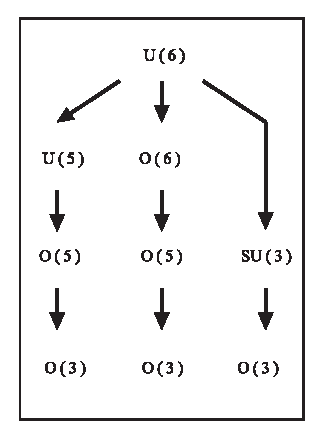
\includegraphics[scale=.65]{figure}
%	%
%	% If no graphics program available, insert a blank space i.e. use
%	%\picplace{5cm}{2cm} % Give the correct figure height and width in cm
%	%
%	%\caption{Please write your figure caption here}
%	\caption{If the width of the figure is less than 7.8 cm use the \texttt{sidecapion} command to flush the caption on the left side of the page. If the figure is positioned at the top of the page, align the sidecaption with the top of the figure -- to achieve this you simply need to use the optional argument \texttt{[t]} with the \texttt{sidecaption} command}
%	\label{fig:2}       % Give a unique label
%\end{figure}


%\begin{table}
%	\caption{Please write your table caption here}
%	\label{tab:1}       % Give a unique label
	%
%\begin{tabular}{p{2cm}p{2.4cm}p{2cm}p{4.9cm}}
%	\hline\noalign{\smallskip}
%	Classes & Subclass & Length & Action Mechanism  \\
%	\noalign{\smallskip}\svhline\noalign{\smallskip}
%	Translation & mRNA$^a$  & 22 (19--25) & Translation repression, mRNA cleavage\\
%	Translation & mRNA cleavage & 21 & mRNA cleavage\\
%	Translation & mRNA  & 21--22 & mRNA cleavage\\
%	Translation & mRNA  & 24--26 & Histone and DNA Modification\\
%	\noalign{\smallskip}\hline\noalign{\smallskip}
%\end{tabular}
%$^a$ Table foot note (with superscript)
%\end{table}


%\begin{svgraybox}
%If you want to emphasize complete paragraphs of texts we recommend to use the newly defined Springer class option \verb|graybox| and the newly defined environment \verb|svgraybox|. This will produce a 15 percent screened box 'behind' your text.
%
%If you want to emphasize complete paragraphs of texts we recommend to use the newly defined Springer class option and environment \verb|svgraybox|. This will produce a 15 percent screened box 'behind' your text.
%\end{svgraybox}


%
%\begin{proof}
%\smartqed
%Proof text goes here.
%\qed
%\end{proof}

%If you want to list definitions or the like we recommend to use the Springer-enhanced \verb|description| environment -- it will automatically render Springer's preferred layout.
%
%\begin{description}[Type 1]
%	\item[Type 1]{That addresses central themes pertainng to migration, health, and disease. In Sect.~\ref{sec:1}, Wilson discusses the role of human migration in infectious disease distributions and patterns.}
%	\item[Type 2]{That addresses central themes pertainng to migration, health, and disease. In Sect.~\ref{subsec:2}, Wilson discusses the role of human migration in infectious disease distributions and patterns.}
%\end{description}

%
